\input{"preamble.tex"}

\addbibresource{Real\_Analysis\_Qual\_Notes.bib}

\let\Begin\begin
\let\End\end
\newcommand\wrapenv[1]{#1}

\makeatletter
\def\ScaleWidthIfNeeded{%
 \ifdim\Gin@nat@width>\linewidth
    \linewidth
  \else
    \Gin@nat@width
  \fi
}
\def\ScaleHeightIfNeeded{%
  \ifdim\Gin@nat@height>0.9\textheight
    0.9\textheight
  \else
    \Gin@nat@width
  \fi
}
\makeatother

\setkeys{Gin}{width=\ScaleWidthIfNeeded,height=\ScaleHeightIfNeeded,keepaspectratio}%

\title{
\textbf{
    Real Analysis Qualifying Exam Review
  }
  }







\begin{document}

\date{}
\maketitle


\newpage

% Note: addsec only in KomaScript
\addsec{Table of Contents}
\tableofcontents
\newpage

\hypertarget{basics}{%
\section{Basics}\label{basics}}

\hypertarget{table-of-notation}{%
\subsection{Table of Notation}\label{table-of-notation}}

\begin{longtable}[]{@{}
  >{\raggedright\arraybackslash}p{(\columnwidth - 2\tabcolsep) * \real{0.85}}
  >{\raggedright\arraybackslash}p{(\columnwidth - 2\tabcolsep) * \real{0.14}}@{}}
\toprule
Notation & Definition \\
\midrule
\endhead
\begin{align*}{\left\lVert {f} \right\rVert}_\infty \coloneqq\sup_{x\in \operatorname{dom}(f)} {\left\lvert {f(x)} \right\rvert}\end{align*}
& The Sup norm \\
\begin{align*} {\left\lVert {f} \right\rVert}_{L^\infty} \coloneqq\inf\left\{{M \geq 0 {~\mathrel{\Big|}~}{\left\lvert {f(x)} \right\rvert} \leq M \text{ for a.e. } x }\right\} \end{align*}
& The \(L^ \infty\) norm \\
\begin{align*} f_n \overset{n \to \infty }\to f \end{align*}
& Convergence of a sequence \\
\begin{align*} f(x) \overset{{\left\lvert {x} \right\rvert} \to \infty}\to 0 \end{align*}
& Vanishing at infinity \\
\begin{align*} \int_{{\left\lvert {x} \right\rvert} \geq N} f \overset{N\to \infty}\to 0 \end{align*}
& Having small tails \\
\begin{align*} H, \mathcal{H} \end{align*}
& A Hilbert space \\
\begin{align*} X \end{align*}
& A topological space \\
\bottomrule
\end{longtable}

\hypertarget{useful-techniques}{%
\subsection{Useful Techniques}\label{useful-techniques}}

\begin{itemize}
\item
  General advice: try swapping the orders of limits, sums, integrals,
  etc.
\item
  Limits:

  \begin{itemize}
  \tightlist
  \item
    Take the \(\limsup\) or \(\liminf\), which always exist, and aim for
    an inequality like
    \begin{align*}  
    c \leq \liminf a_n \leq \limsup a_n \leq c
    .\end{align*}
  \item
    \(\lim f_n = \limsup f_n = \liminf f_n\) iff the limit exists, so to
    show some \(g\) is a limit, show
    \begin{align*}  
    \limsup f_n \leq g \leq \liminf f_n \qquad (\implies g = \lim f) 
    .\end{align*}
  \item
    A limit does \emph{not} exist if \(\liminf a_n > \limsup a_n\).
  \end{itemize}
\item
  Sequences and Series

  \begin{itemize}
  \tightlist
  \item
    If \(f_n\) has a global maximum (computed using \(f_n'\) and the
    first derivative test) \(M_n \to 0\), then \(f_n \to 0\) uniformly.
  \item
    For a fixed \(x\), if \(f = \sum f_n\) converges \emph{uniformly} on
    some \(B_r(x)\) and each \(f_n\) is continuous at \(x\), then \(f\)
    is also continuous at \(x\) .
  \end{itemize}
\item
  Equalities

  \begin{itemize}
  \tightlist
  \item
    Split into upper and lower bounds:
    \begin{align*}  
    a=b \iff a\leq b \text{ and }  a\geq b
    .\end{align*}
  \item
    Use an epsilon of room:
    \begin{align*}  
    \qty{ \forall \epsilon, \,\,a < b + {\varepsilon}} \implies a\leq b 
    .\end{align*}
  \item
    Showing something is zero:
    \begin{align*}  
    \qty{ \forall \epsilon, \,\, {\left\lVert {a} \right\rVert} < {\varepsilon}} \implies a = 0
    .\end{align*}
  \end{itemize}
\item
  Continuity / differentiability: show it holds on \([-M, M]\) for all
  \(M\) to get it to hold on \({\mathbb{R}}\).
\item
  Simplifications:

  \begin{itemize}
  \tightlist
  \item
    To show something for a measurable set, show it for
    bounded/compact/elementary sets/
  \item
    To show something for a function, show it for continuous, bounded,
    compactly supported, simple, chi functions, \(L^1\), etc
  \item
    Replace a continuous sequence (\({\varepsilon}\to 0\)) with an
    arbitrary countable sequence (\(x_n \to 0\))
  \item
    Intersect with a ball \(B_r(\mathbf{0})\subset {\mathbb{R}}^n\).
  \end{itemize}
\item
  Integrals

  \begin{itemize}
  \tightlist
  \item
    Calculus techniques: Taylor series, IVT, MVT, etc.
  \item
    Break up
    \({\mathbb{R}}^n = \left\{{{\left\lvert {x} \right\rvert} \leq 1}\right\} \coprod \left\{{{\left\lvert {x} \right\rvert} > 1}\right\}\).

    \begin{itemize}
    \tightlist
    \item
      Or break integration region into disjoint annuli.
    \end{itemize}
  \item
    Break up into
    \(\left\{{f>g}\right\} {\textstyle\coprod}\left\{{f=g}\right\} {\textstyle\coprod}\left\{{f< g}\right\}\).
  \item
    Tail estimates!
  \item
    Most of what works for integrals will work for sums.
  \end{itemize}
\item
  Measure theory:

  \begin{itemize}
  \item
    Always consider bounded sets, and if \(E\) is unbounded write
    \(E = \cup_{n} B_{n}(0) \cap E\) and use countable subadditivity or
    continuity of measure.
  \item
    \(F_\sigma\) sets are Borel, so establish something for Borel sets
    and use this to extend it to Lebesgue.
  \item
    \(s = \inf\left\{{x\in X}\right\} \implies\) for every
    \(\varepsilon\) there is an \(x\in X\) such that
    \(x \leq s + \varepsilon\).
  \end{itemize}
\item
  Approximate by dense subsets of functions
\item
  Useful facts about compactly supported (\(C_c({\mathbb{R}})\))
  continuous functions:

  \begin{itemize}
  \tightlist
  \item
    Uniformly continuous
  \item
    Bounded almost everywhere
  \end{itemize}
\end{itemize}

\hypertarget{definitions}{%
\subsection{Definitions}\label{definitions}}

\begin{definition}[Completeness]

A metric space is \textbf{complete} if every Cauchy sequence converges.

\end{definition}

\begin{fact}

If \(X\) is complete, then absolutely convergent implies convergent.

\end{fact}

\begin{definition}[Continuity and Uniform Continuity]

A function \(f: {\mathbb{R}}\to {\mathbb{R}}\) is \textbf{continuous} on
a set \(X\) iff
\begin{align*}
\forall x_0 \in X, \forall {\varepsilon}>0, \quad \exists\delta = \delta(x_0, {\varepsilon}) >0 \quad\text{ such that }\quad \forall x\in X, \, {\left\lvert {x-x_0} \right\rvert}<\delta \implies {\left\lvert {f(x) - f(x_0)} \right\rvert} < {\varepsilon}
.\end{align*}

\(f\) is \textbf{uniformly continuous} iff

\begin{align*}
  &\forall \varepsilon \quad \exists \delta(\varepsilon) \text{ such that }\quad \forall x, y, \in X \quad {\left\lvert {x - y} \right\rvert} < \delta \implies {\left\lvert {f(x) - f(y)} \right\rvert} < \varepsilon \\
\iff &\forall \varepsilon \quad \exists \delta(\varepsilon) \mathrel{\Big|}\quad \forall x, y, \quad {\left\lvert {y} \right\rvert} < \delta \implies {\left\lvert {f(x-y) - f(y)} \right\rvert} < \varepsilon
.\end{align*}

\end{definition}

\begin{remark}

The main difference is that \(\delta\) may depend on \(x_0\) and
\({\varepsilon}\) in continuity, but only depends on \({\varepsilon}\)
in the uniform version. I.e. once \(\delta\) is fixed, for continuity
one may only range over \(x\), but in uniform continuity one can range
over all pairs \(x,y\).

\end{remark}

\begin{proposition}[Lipschitz implies uniformly continuous]

If \(f\) is Lipschitz on \(X\), then \(f\) is uniformly continuous on
\(X\).

Supposing that
\begin{align*}
{\left\lVert {f(x) - f(y)} \right\rVert} \leq C {\left\lVert {x-y} \right\rVert}
,\end{align*}
for a fixed \({\varepsilon}\) take
\(\delta({\varepsilon}) \coloneqq{\varepsilon}/C\), then
\begin{align*}
{\left\lVert {f(x) - f(y)} \right\rVert}
&\leq C {\left\lVert {x-y} \right\rVert} \\
&\leq C \delta \\
&= C \qty{{\varepsilon}/C} \\
&= {\varepsilon}
.\end{align*}

\end{proposition}

\begin{definition}[Nowhere Dense Sets]

A set \(S\) is \textbf{nowhere dense} iff the closure of \(S\) has empty
interior iff every interval contains a subinterval that does not
intersect \(S\).

\end{definition}

\begin{definition}[Meager Sets]

A set is \textbf{meager} if it is a \emph{countable} union of nowhere
dense sets.

\end{definition}

\begin{definition}[$F_\sigma$ and $G_\delta$ Sets]

An \(F_\sigma\) set is a union of closed sets, and a \(G_\delta\) set is
an intersection of opens. \footnote{Mnemonic: ``F'' stands for
  \emph{ferme}, which is ``closed'' in French, and \(\sigma\)
  corresponds to a ``sum'', i.e.~a union.}

\end{definition}

\begin{definition}[Limsup/Liminf]

\begin{align*}  
\limsup_n a_n = \lim_{n\to \infty} \sup_{j\geq n} a_j &= \inf_{n\geq 0} \sup_{j\geq n} a_j \\ 
\liminf_n a_n = \lim_{n\to \infty} \inf_{j\geq n} a_j &= \sup_{n\geq 0} \inf_{j\geq n} a_j
.\end{align*}

\end{definition}

\begin{definition}[Topological Notions]

Let \(X\) be a metric space and \(A\) a subset. Let \(A'\) denote the
limit points of \(A\), and
\(\mkern 1.5mu\overline{\mkern-1.5muA\mkern-1.5mu}\mkern 1.5mu \coloneqq A\cup A'\)
to be its closure.

\begin{itemize}
\item
  A \textbf{neighborhood} of \(p\) is an open set \(U_p\) containing
  \(p\).
\item
  An \({\varepsilon}{\hbox{-}}\)\textbf{neighborhood} of \(p\) is an
  open ball
  \(B_r(p) \coloneqq\left\{{q {~\mathrel{\Big|}~}d(p, q) < r}\right\}\)
  for some \(r>0\).
\item
  A point \(p\in X\) is an \textbf{accumulation point} of \(A\) iff
  every neighborhood \(U_p\) of \(p\) contains a point \(q\in Q\)
\item
  A point \(p\in X\) is a \textbf{limit point} of \(A\) iff every
  \emph{punctured} neighborhood \(U_p\setminus\left\{{p}\right\}\)
  contains a point \(q\in A\).
\item
  If \(p\in A\) and \(p\) is not a limit point of \(A\), then \(p\) is
  an \textbf{isolated point} of \(A\).
\item
  \(A\) is \textbf{closed} iff \(A' \subset A\), so \(A\) contains all
  of its limit points.
\item
  A point \(p\in A\) is \textbf{interior} iff there is a neighborhood
  \(U_p \subset A\) that is strictly contained in \(A\).
\item
  \(A\) is \textbf{open} iff every point of \(A\) is interior.
\item
  \(A\) is \textbf{perfect} iff \(A\) is closed and \(A\subset A'\), so
  every point of \(A\) is a limit point of \(A\).
\item
  \(A\) is \textbf{bounded} iff there is a real number \(M\) and a point
  \(q\in X\) such that \(d(p, q) < M\) for all \(p\in A\).
\item
  \(A\) is \textbf{dense} in \(X\) iff every point \(x\in X\) is either
  a point of \(A\), so \(x\in A\), or a limit point of \(A\), so
  \(x\in A'\). I.e., \(X\subset A\cup A'\).

  \begin{itemize}
  \tightlist
  \item
    Alternatively,
    \(\mkern 1.5mu\overline{\mkern-1.5muA\mkern-1.5mu}\mkern 1.5mu = X\),
    so the closure of \(A\) is \(X\).
  \end{itemize}
\end{itemize}

\end{definition}

\begin{definition}[Uniform Convergence]

\begin{align*}
(\forall \varepsilon>0)\left(\exists n_{0} = n_0({\varepsilon}) \right)(\forall x \in S)\left(\forall n>n_{0}\right)\left(\left|f_{n}(x)-f(x)\right|<\varepsilon\right)
.\end{align*}
Negated:\footnote{Slogan: to negate, find a bad \(x\) depending on
  \(n_0\) that are larger than some \({\varepsilon}\).}
\begin{align*}  
(\exists \varepsilon>0)\left(\forall n_{0} = n_0 ({\varepsilon}) \right)(\exists x = x(n_0) \in S)\left(\exists n>n_{0}\right)\left(\left|f_{n}(x)-f(x)\right| \geq \varepsilon\right)
.\end{align*}

\end{definition}

\begin{definition}[Pointwise Convergence]

A sequence of functions \(\left\{{ f_j }\right\}\) is said to
\textbf{converge pointwise} to \(f\) if and only if
\begin{align*}  
(\forall \varepsilon>0)(\forall x \in S)\left(\exists n_{0} = n_0(x, {\varepsilon}) \right)\left(\forall n>n_{0}\right)\left(\left|f_{n}(x)-f(x)\right|<\varepsilon\right)
.\end{align*}

\end{definition}

\begin{proposition}[Implications of convergence]

Uniform \(\implies\) pointwise \(\implies\) almost everywhere
\(\implies\) (roughly) \(L^1\) convergence. Why these can't be reversed:

\begin{itemize}
\tightlist
\item
  Pointwise but not uniform???: \({1\over n}\one_{[0, n]}\)
\item
  Almost everywhere but not pointwise???: \(n \one_{[0, {1\over n} ] }\)
\item
  \(n \chi_{[n, n+1]}\)????
\end{itemize}

\end{proposition}

\begin{definition}[Outer Measure]

The \textbf{outer measure} of a set is given by
\begin{align*}
m_*(E) \coloneqq\inf_{\substack{\left\{{Q_{i}}\right\} \rightrightarrows E \\ \text{closed cubes}}} \sum {\left\lvert {Q_{i}} \right\rvert}
.\end{align*}

\end{definition}

\begin{definition}[Limsup and Liminf of Sets]

\begin{align*}
\liminf_{n} E_{n} \coloneqq\displaystyle\bigcup_{N=1}^\infty \displaystyle\bigcap_{n=N}^\infty E_{n} &= \left\{{x {~\mathrel{\Big|}~}x\in E_{n} \text{ for all but finitely many } n}\right\}  \\
\limsup_{n} E_{n} \coloneqq\displaystyle\bigcap_{N=1}^\infty \displaystyle\bigcup_{n=N}^{\infty} E_{n} &= \left\{{x {~\mathrel{\Big|}~}x\in E_{n} \text{ for infinitely many } n}\right\}  \\
.\end{align*}

How to derive these definitions:

\begin{itemize}
\tightlist
\item
  For
  \(A \coloneqq\displaystyle\bigcup_{N=1}^\infty \displaystyle\bigcap_{n=N}^\infty E_n\):

  \begin{itemize}
  \tightlist
  \item
    \(x\in A \iff\) there exists some \(N\) such that
    \(x\in \cap_{n\geq N} E_n\), i.e.~\(x\in E_n\) for all \(n\geq N\).
    So \(x\) is in \emph{all} but finitely many \(n\).
  \end{itemize}
\item
  For
  \(B \coloneqq\displaystyle\bigcap{N=1}^\infty \displaystyle\bigcup{n=N}^\infty E_n\):

  \begin{itemize}
  \tightlist
  \item
    \(x\in B \iff\) for every \(N\), there exists some \(n\geq N\) such
    that \(x\in E_n\). So \(x\) is an infinitely many \(E_n\).
  \end{itemize}
\end{itemize}

Note that \(A\subseteq B\) since being in all but finitely many \(E_n\)
necessarily implies being in infinitely many. This corresponds to
\(\liminf_n E_n \subseteq \limsup_n E_n\).

\end{definition}

\begin{definition}[Lebesgue Measurable Sets]

A subset \(E\subseteq {\mathbb{R}}^n\) is \textbf{Lebesgue measurable}
iff for every \({\varepsilon}> 0\) there exists an open set
\(O \supseteq E\) such that \(m_*(O\setminus E) < {\varepsilon}\). In
this case, we define \(m(E) \coloneqq m_*(E)\).

\end{definition}

\begin{definition}[$L^+$: Measurable non-negative functions.]

\(f\in L^+\) iff \(f\) is measurable and non-negative.

\end{definition}

\begin{definition}[Integrability]

A measurable function is \textbf{integrable} iff
\({\left\lVert {f} \right\rVert}_1 < \infty\).

\end{definition}

\begin{definition}[The Infinity Norm]

\begin{align*}
{\left\lVert {f} \right\rVert}_\infty &\coloneqq\inf_{\alpha \geq 0} \left\{{\alpha {~\mathrel{\Big|}~}m\left\{{{\left\lvert {f} \right\rvert} \geq \alpha}\right\} = 0}\right\}
.\end{align*}

\end{definition}

\begin{definition}[Essentially Bounded Functions]

A function \(f:X \to {\mathbb{C}}\) is \textbf{essentially bounded} iff
there exists a real number \(c\) such that
\(\mu(\left\{{{\left\lvert {f} \right\rvert} > x}\right\}) = 0\),
i.e.~\({\left\lVert {f} \right\rVert}_\infty < \infty\).

\end{definition}

\begin{definition}[$L^\infty$]

\begin{align*}
L^\infty(X)
\coloneqq\left\{{f: X\to {\mathbb{C}}{~\mathrel{\Big|}~}f \text{ is essentially bounded }}\right\}
\coloneqq\left\{{f: X\to {\mathbb{C}}{~\mathrel{\Big|}~}{\left\lVert {f} \right\rVert}_{\infty }< \infty}\right\}
.\end{align*}

\end{definition}

\begin{definition}[Dual Norm]

For \(X\) a normed vector space and \(\Lambda \in X {}^{ \vee }\),
\begin{align*}
{\left\lVert {\Lambda} \right\rVert}_{X {}^{ \vee }} \coloneqq\sup_{\left\{{x\in X {~\mathrel{\Big|}~}{\left\lVert {x} \right\rVert}_X \leq 1}\right\}} {\left\lvert {f(x)} \right\rvert}
.\end{align*}

\end{definition}

\begin{definition}[Convolution]

\begin{align*}f * g(x)=\int f(x-y) g(y) d y .\end{align*}

\end{definition}

\begin{definition}[Fourier Transform]

\begin{align*}
\widehat{f}(\xi) = \int f(x) ~e^{2\pi i x \cdot \xi} ~dx
.\end{align*}

\end{definition}

\begin{definition}[Dilation]

\begin{align*}
\phi_{t}(x) = t^{-n} \phi\left(t^{-1} x\right)
.\end{align*}

\end{definition}

\begin{definition}[Approximations to the identity]

For \(\phi\in L^1\), the dilations satisfy
\(\int \phi_{t} = \int \phi\), and if \(\int \phi = 1\) then \(\phi\) is
an \textbf{approximate identity}.

\end{definition}

\begin{definition}[Baire Space]

A space \(X\) is a \textbf{Baire space} if and only if every countable
intersections of open, dense sets is still dense.

\end{definition}

\hypertarget{functional-analysis}{%
\subsubsection{Functional Analysis}\label{functional-analysis}}

\begin{definition}[Orthonormal sequence ]

A countable collection of elements \(\left\{{ u_i }\right\}\) is
\textbf{orthonormal} if and only if

\begin{enumerate}
\def\labelenumi{\arabic{enumi}.}
\tightlist
\item
  \({\left\langle {u_i},~{u_j} \right\rangle} = 0\) for all \(j \neq k\)
  and
\item
  \({\left\lVert {u_j} \right\rVert}^2 \coloneqq{\left\langle {u_j},~{u_j} \right\rangle} = 1\)
  for all \(j\).
\end{enumerate}

\end{definition}

\begin{definition}[Basis of a Hilbert space]

A set \(\left\{{u_{n}}\right\}\) is a \textbf{basis} for a Hilbert space
\({\mathcal{H}}\) iff it is dense in \({\mathcal{H}}\).

\end{definition}

\begin{definition}[Completeness of a Hilbert space]

A collection of vectors \(\left\{{u_{n}}\right\}\subset H\) is
\textbf{complete} iff \({\left\langle {x},~{u_{n}} \right\rangle} = 0\)
for all \(n \iff x = 0\) in \(H\).

\end{definition}

\begin{definition}[Dual of a Hilbert space]

The \textbf{dual} of a Hilbert space \(H\) is defined as
\begin{align*}
H {}^{ \vee }\coloneqq\left\{{L: H\to {\mathbb{C}}{~\mathrel{\Big|}~}L \text{ is continuous }}\right\}
.\end{align*}

\end{definition}

\begin{definition}[Linear functionals]

A map \(L: X \to {\mathbb{C}}\) is a \textbf{linear functional} iff
\begin{align*}
L(\alpha\mathbf{x} + \mathbf{y}) = \alpha L(\mathbf{x}) + L(\mathbf{y}).
.\end{align*}

\end{definition}

\begin{definition}[Operator norm]

The \textbf{operator norm} of an operator \(L\) is defined as
\begin{align*}
{\left\lVert {L} \right\rVert}_{X {}^{ \vee }} \coloneqq\sup_{ \substack{x\in X \\ {\left\lVert {x} \right\rVert} = 1} } {\left\lvert {L(x)} \right\rvert}
.\end{align*}

\end{definition}

\begin{definition}[Banach Space]

A space is a \textbf{Banach space} if and only if it is a complete
normed vector space.

\end{definition}

\begin{definition}[Hilbert Space]

A \textbf{Hilbert space} is an inner product space which is a Banach
space under the induced norm.

\end{definition}

\hypertarget{theorems}{%
\subsection{Theorems}\label{theorems}}

\begin{theorem}[Folland 0.25]

For \(E \subseteq (X, d)\) a metric space, TFAE:

\begin{itemize}
\tightlist
\item
  \(E\) is complete and totally bounded.
\item
  \(E\) is sequentially compact: Every sequence in \(E\) has a
  subsequence that converges to a point in \(E\).
\item
  \(E\) is compact: every open cover has a finite subcover.
\end{itemize}

Note that \(E\) is complete as a metric space with the induced metric
iff \(E\) is closed in \(X\), and \(E\) is bounded iff it is totally
bounded.

\end{theorem}

\begin{theorem}[Mean Value Theorem]

If \(f: [a, b] \to {\mathbb{R}}\) is continuous on a closed interval and
differentiable on \((a, b)\), then there exists \(\xi \in [a, b]\) such
that
\begin{align*}
f(b) - f(a) = f'(\xi)(b-a)
.\end{align*}

\end{theorem}

\begin{theorem}[Lagrange and Cauchy Remainders]

If \(f\) is \(n\) times differentiable on a neighborhood of a point
\(p\), say \(N_\delta(p)\), then for all points \(x\) in the deleted
neighborhood \(N_\delta(p) - \left\{{p}\right\}\) , there exists a point
\(\xi\) strictly between \(x\) and \(p\) such that
\begin{align*}
x \in N_\delta(p)-\left\{{p}\right\} \implies f(x) 
&= \sum_{k=0}^{n-1} \frac{f^{(k)}(p)}{k!}(x-p)^k + \frac{f^{(n)}(\xi)}{n!}(x-p)^n \\ \\
&= \sum_{k=0}^{n-1} \frac{f^{(k)}(p)}{k!}(x-p)^k + \int_c^x \frac{1}{n!} {\frac{\partial ^n f}{\partial x^n}\,}(t) (x-t)^n ~dt
\end{align*}

\end{theorem}

\begin{proposition}[Sufficient condition for Taylor convergence]

Given a point \(c\) and some \(\varepsilon>0\), if \(f \in C^\infty(I)\)
and there exists an \(M\) such that
\begin{align*}
x \in N_\varepsilon(c) \implies {\left\lvert {f^{(n)}(x)} \right\rvert} \leq M^n
\end{align*}
then the Taylor expansion about \(c\) converges on \(N_\varepsilon(c)\).

\end{proposition}

\hypertarget{topology-sets}{%
\subsubsection{Topology / Sets}\label{topology-sets}}

\begin{theorem}[Heine-Cantor]

Every continuous function \(f:X\to Y\) where \(X\) is a compact metric
space is uniformly continuous.

\end{theorem}

\begin{proof}[?]

Fix \({\varepsilon}>0\), we'll find a \(\delta\) that works for all
\(x\in X\) uniformly. For every \(x\in X\), pick a \(\delta_x\)
neighborhood satisfying the conditions for (assumed) continuity. Take an
open cover by \(\delta_x/2\) balls, extract a finite subcover, take
\(\delta\) the minimal radius.

\end{proof}

\begin{proposition}[Compact if and only if sequentially compact for metric spaces]

Metric spaces are compact iff they are sequentially compact, (i.e.~every
sequence has a convergent subsequence).

\end{proposition}

\begin{proof}[?]

Todo. \todo[inline]{Proof.}

\end{proof}

\begin{proposition}[A unit ball that is not compact]

The unit ball in \(C([0, 1])\) with the sup norm is not compact.

\end{proposition}

\begin{proof}[?]

Take \(f_k(x) = x^n\), which converges to \(\chi(x=1)\). The limit is
not continuous, so no subsequence can converge.

\end{proof}

\begin{proposition}[?]

A \emph{finite} union of nowhere dense is again nowhere dense.

\end{proposition}

\begin{proposition}[Convergent Sums Have Small Tails]

\begin{align*}\sum a_n < \infty \implies a_n \to 0 {\quad \operatorname{and} \quad} \sum_{k=N}^\infty a_n \overset{N\to\infty}\to 0\end{align*}

\end{proposition}

\begin{theorem}[Heine-Borel]

\(X\subseteq {\mathbb{R}}^n\) is compact \(\iff X\) is closed and
bounded.

\end{theorem}

\begin{proposition}[Geometric Series]

\begin{align*}
\sum_{k=0}^\infty x^k = \frac 1 {1-x} \iff {\left\lvert {x} \right\rvert} < 1
.\end{align*}

\end{proposition}

\begin{corollary}[?]

\begin{align*}
\sum_{k=0}^\infty \frac 1 {2^k} = 1
.\end{align*}

\end{corollary}

\begin{proposition}[?]

The Cantor set is closed with empty interior.

\end{proposition}

\begin{proof}[?]

Its complement is a union of open intervals, and can't contain an
interval since intervals have positive measure and \(m(C_n)\) tends to
zero.

\end{proof}

\begin{corollary}[?]

The Cantor set is nowhere dense.

\end{corollary}

\begin{proposition}[?]

Singleton sets in \({\mathbb{R}}\) are closed, and thus \({\mathbb{Q}}\)
is an \(F_\sigma\) set.

\end{proposition}

\begin{theorem}[Baire]

\({\mathbb{R}}\) is a \textbf{Baire space} Thus \({\mathbb{R}}\) can not
be written as a countable union of nowhere dense sets.

\end{theorem}

\begin{lemma}[?]

Any nonempty set which is bounded from above (resp. below) has a
well-defined supremum (resp. infimum).

\end{lemma}

\hypertarget{functions}{%
\subsubsection{Functions}\label{functions}}

\begin{proposition}[Existence of Smooth Compactly Supported Functions]

There exist smooth compactly supported functions, e.g.~take
\begin{align*}
f(x) = e^{-\frac{1}{x^2}} \chi_{(0, \infty)}(x)
.\end{align*}

\end{proposition}

\begin{lemma}[Function discontinuous on the rationals]

There is a function discontinuous precisely on \({\mathbb{Q}}\).

\end{lemma}

\begin{proof}[?]

\(f(x) = \frac 1 n\) if \(x = r_n \in {\mathbb{Q}}\) is an enumeration
of the rationals, and zero otherwise. The limit at every point is 0.

\end{proof}

\begin{proposition}[No functions discontinuous on the irrationals]

There \emph{do not} exist functions that are discontinuous precisely on
\({\mathbb{R}}\setminus {\mathbb{Q}}\).

\end{proposition}

\begin{proof}[?]

\(D_f\) is always an \(F_\sigma\) set, which follows by considering the
oscillation \(\omega_f\). \(\omega_f(x) = 0 \iff f\) is continuous at
\(x\), and \(D_f = \cup_n A_{\frac 1 n}\) where
\(A_\varepsilon = \left\{{\omega_f \geq \varepsilon}\right\}\) is
closed.

\end{proof}

\begin{proposition}[Lipschitz $\iff$ differentiable with bounded derivative.]

A function \(f: (a, b) \to {\mathbb{R}}\) is Lipschitz \(\iff f\) is
differentiable and \(f'\) is bounded. In this case,
\({\left\lvert {f'(x)} \right\rvert} \leq C\), the Lipschitz constant.

\end{proposition}

\hypertarget{sequences-and-series}{%
\subsubsection{Sequences and Series}\label{sequences-and-series}}

\begin{proposition}[The Cauchy condensation test]

For \(\left\{{a_k}\right\}\) is a non-increasing sequence in
\({\mathbb{R}}\) then
\begin{align*}
\sum_{k\geq 1} a_k < \infty \iff \sum_{k\geq 1} 2^k a_{2^k}<\infty
.\end{align*}

\end{proposition}

\begin{proof}[?]

Show that
\begin{align*}
\sum a_k \leq \sum 2^k a_{2^k} \leq 2 \sum a_k
\end{align*}
using
\begin{align*}
\sum a_k = a_0 + a_1 + a_2 + a_3 + \cdots
\leq \qty{a_1} + \qty{a_2 + a_2} + {a_3 + a_3 + a_3 + a_3} + \cdots \\
\end{align*}
where each group with \(a_k\) has \(2^k\) terms.

\end{proof}

\hypertarget{uniform-convergence}{%
\subsection{Uniform Convergence}\label{uniform-convergence}}

\begin{proposition}[Testing Uniform Convergence: The Sup Norm Test]

\(f_n \to f\) uniformly iff there exists an \(M_n\) such that
\({\left\lVert {f_n - f} \right\rVert}_\infty \leq M_n \to 0\).

\end{proposition}

\begin{remark}[Negating the Sup Norm test]

\textbf{Negating}: find an \(x\) which depends on \(n\) for which
\({\left\lVert {f_n} \right\rVert}_\infty > {\varepsilon}\) (negating
small tails) or
\({\left\lVert {f_n - f_m} \right\rVert} > {\varepsilon}\) (negating the
Cauchy criterion).

\end{remark}

\begin{proposition}[$C(I)$ is complete]

The space \(X = C([0, 1])\), continuous functions
\(f: [0, 1] \to {\mathbb{R}}\), equipped with the norm
\begin{align*}
{\left\lVert {f} \right\rVert}_\infty \coloneqq\sup_{x\in [0, 1]} {\left\lvert {f(x)} \right\rvert}
\end{align*}
is a \textbf{complete} metric space.

\end{proposition}

\begin{proof}

\envlist

\begin{enumerate}
\def\labelenumi{\arabic{enumi}.}
\item
  Let \(\left\{{f_k}\right\}\) be Cauchy in \(X\).
\item
  Define a candidate limit using pointwise convergence:

  Fix an \(x\); since
  \begin{align*}
    {\left\lvert {f_k(x) - f_j(x)} \right\rvert}  \leq {\left\lVert {f_k - f_k} \right\rVert} \to 0
    \end{align*}
  the sequence \(\left\{{f_k(x)}\right\}\) is Cauchy in
  \({\mathbb{R}}\). So define \(f(x) \coloneqq\lim_k f_k(x)\).
\item
  Show that \({\left\lVert {f_k - f} \right\rVert} \to 0\):
  \begin{align*}
    {\left\lvert {f_k(x) - f_j(x)} \right\rvert} < \varepsilon ~\forall x \implies \lim_{j} {\left\lvert {f_k(x) - f_j(x)} \right\rvert} <\varepsilon ~\forall x
    \end{align*}
  Alternatively,
  \({\left\lVert {f_k-f} \right\rVert} \leq {\left\lVert {f_k - f_N} \right\rVert} + {\left\lVert {f_N - f_j} \right\rVert}\),
  where \(N, j\) can be chosen large enough to bound each term by
  \(\varepsilon/2\).
\item
  Show that \(f\in X\):

  The uniform limit of continuous functions is continuous.
\end{enumerate}

\end{proof}

\begin{remark}

In other cases, you may need to show the limit is bounded, or has
bounded derivative, or whatever other conditions define \(X\).

\end{remark}

\begin{theorem}[Uniform Limit Theorem]

If \(f_n\to f\) pointwise and uniformly with each \(f_n\) continuous,
then \(f\) is continuous. \footnote{Slogan: a uniform limit of
  continuous functions is continuous.}

\end{theorem}

\begin{proof}

\envlist

\begin{itemize}
\item
  Follows from an \(\varepsilon/3\) argument:
  \begin{align*}  
  {\left\lvert {F(x) - F(y} \right\rvert} \leq 
  {\left\lvert {F(x) - F_N(x)} \right\rvert} + {\left\lvert {F_N(x) - F_N(y)} \right\rvert} + {\left\lvert {F_N(y) - F(y)} \right\rvert} 
  \leq {\varepsilon}\to 0
  .\end{align*}

  \begin{itemize}
  \tightlist
  \item
    The first and last \({\varepsilon}/3\) come from uniform convergence
    of \(F_N\to F\).
  \item
    The middle \({\varepsilon}/3\) comes from continuity of each
    \(F_N\).
  \end{itemize}
\item
  So just need to choose \(N\) large enough and \(\delta\) small enough
  to make all 3 \(\varepsilon\) bounds hold.
\end{itemize}

\end{proof}

\begin{proposition}[Uniform Limits Commute with Integrals]

If \(f_n \to f\) uniformly, then \(\int f_n = \int f\).

\end{proposition}

\hypertarget{series}{%
\subsubsection{Series}\label{series}}

\begin{proposition}[p-tests]

Let \(n\) be a fixed dimension and set
\(B = \left\{{x\in {\mathbb{R}}^n {~\mathrel{\Big|}~}{\left\lVert {x} \right\rVert} \leq 1}\right\}\).
\begin{align*}
\sum \frac 1 {n^p} < \infty &\iff p>1 \\
\int_\varepsilon^\infty \frac 1 {x^p} < \infty 
&\iff p>1 \\
\int_0^1 \frac 1 {x^p} < \infty 
&\iff p<1 \\
\int_B \frac{1}{{\left\lvert {x} \right\rvert}^p} < \infty &\iff p < n \\
\int_{B^c} \frac{1}{{\left\lvert {x} \right\rvert}^p} < \infty &\iff p > n \\
.\end{align*}

\end{proposition}

\begin{proposition}[Comparison Test]

If \(0\leq a_n \leq b_n\), then

\begin{itemize}
\tightlist
\item
  \(\sum b_n < \infty \implies \sum a_n < \infty\), and
\item
  \(\sum a_n = \infty \implies \sum b_n = \infty\).
\end{itemize}

\end{proposition}

\begin{proposition}[Small Tails for Series of Functions]

If \(\sum f_n\) converges then \(f_n \to 0\) uniformly.

\end{proposition}

\begin{corollary}[Term by Term Continuity Theorem]

If \(f_n\) are continuous and \(\sum f_n \to f\) converges uniformly,
then \(f\) is continuous.

\end{corollary}

\begin{proposition}[Weak $M\dash$Test]

If \(f_n(x) \leq M_n\) \textbf{for a fixed \(x\)} where
\(\sum M_n < \infty\), then the series \(f(x) = \sum f_n(x)\)
converges.\footnote{Note that this is only pointwise convergence of
  \(f\), whereas the full \(M{\hbox{-}}\)test gives uniform convergence.}

\end{proposition}

\begin{proposition}[The Weierstrass $M\dash$Test]

If \(\sup_{x\in A} {\left\lvert {f_n(x)} \right\rvert} \leq M_n\) for
each \(n\) where \(\sum M_n < \infty\), then
\(\sum_{n=1}^\infty f_n(x)\) converges uniformly and absolutely on
\(A\). \footnote{It suffices to show
  \({\left\lvert {f_n(x)} \right\rvert} \leq M_n\) for some \(M_n\) not
  depending on \(x\).} Conversely, if \(\sum f_n\) converges uniformly
on \(A\) then
\(\sup_{x\in A} {\left\lvert {f_n(x)} \right\rvert} \to 0\).

\end{proposition}

\begin{proposition}[Cauchy criterion for sums]

\(f_n\) are uniformly Cauchy (so
\({\left\lVert {f_n - f_m} \right\rVert}_\infty < {\varepsilon}\)) iff
\(f_n\) is uniformly convergent.

\end{proposition}

\hypertarget{derivatives}{%
\paragraph{Derivatives}\label{derivatives}}

\begin{theorem}[Term by Term Differentiability Theorem]

If \(f_n\) are differentiable, \(\sum f_n' \to g\) uniformly, and there
exists one point\footnote{So this implicitly holds if \(f\) is the
  pointwise limit of \(f_n\).} \(x_0\) such that \(\sum f_n(x)\)
converges, then there exist an \(f\) such that \(\sum f_n \to f\)
uniformly and \(f' = g\).\footnote{See Abbott theorem 6.4.3, pp 168.}

\end{theorem}

\hypertarget{commuting-limiting-operations}{%
\subsection{Commuting Limiting
Operations}\label{commuting-limiting-operations}}

\begin{proposition}[Limits of bounded functions need not be bounded]

\begin{align*}  
\lim_{n\to \infty}\sup_{x\in X} {\left\lvert {f_n(x) } \right\rvert} \neq \sup_{x\in X} {\left\lvert {\lim_{n\to\infty} f_n(x) } \right\rvert}
.\end{align*}

\end{proposition}

\begin{proposition}[Limits of continuous functions need not be continuous]

\begin{align*}  
\lim_{k\to \infty} \lim_{n\to\infty} f_n(x_k) \neq
\lim_{n\to \infty} \lim_{k\to\infty} f_n(x_k)
.\end{align*}

\end{proposition}

\begin{proposition}[Limits of differentiable functions need not be differentiable]

\begin{align*}  
\lim_{n\to \infty} {\frac{\partial }{\partial x}\,} f_n \neq {\frac{\partial }{\partial n}\,} \qty{\lim_{n\to \infty} f_n}
.\end{align*}
Note that uniform convergence of \(f_n\) and \(f_n'\) is sufficient to
guarantee that \(f\) is differentiable. Even worse: every continuous
function is a uniform limit of polynomials by the Weierstrass
approximation theorem.

\end{proposition}

\begin{example}[?]

As a counterexample:
\begin{align*}
f_n(x) \coloneqq\sqrt{x^2 + {1\over n}} \overset{n\to\infty}\longrightarrow f(x) \coloneqq{\left\lvert {x} \right\rvert}
,\end{align*}
and this convergence is even uniform.

\end{example}

\begin{example}[?]

\begin{align*}
f_n(x) \coloneqq{x\over 1 + nx^2}
.\end{align*}
Then by Calculus, \(f_n(x) \leq 1/2\sqrt{n} \coloneqq M_n\) and
\(f_n\to 0\) uniformly, so \(f' = 0\). But
\begin{align*}
f_n'(x) = {1-nx^2 \over\qty{1 + nx^2}^2}
,\end{align*}
and \(f_n'(0) \to 1\).

\end{example}

\begin{proposition}[?]

\begin{align*}  
\lim_{n\to \infty} \int_a^b f_n(x) \,dx \neq \int_a^b \lim_{n\to \infty} \qty{ f_n(x) } \,dx
.\end{align*}

\end{proposition}

\hypertarget{almost-theorems}{%
\subsection{``Almost'' Theorems}\label{almost-theorems}}

\begin{theorem}[Egorov's Theorem]

Let \(E \subseteq {\mathbb{R}}^d\) be measurable of positive finite
measure with \(f_k\to f\) almost everywhere on \(E\). Then for every
\({\varepsilon}> 0\) there is a closed \(A_{\varepsilon}\subseteq E\)
with \(\mu(E\setminus A_{\varepsilon}) < {\varepsilon}\) and
\(f_k\to f\) uniformly on \(A_{\varepsilon}\).

\end{theorem}

\begin{proof}[of Egorov]

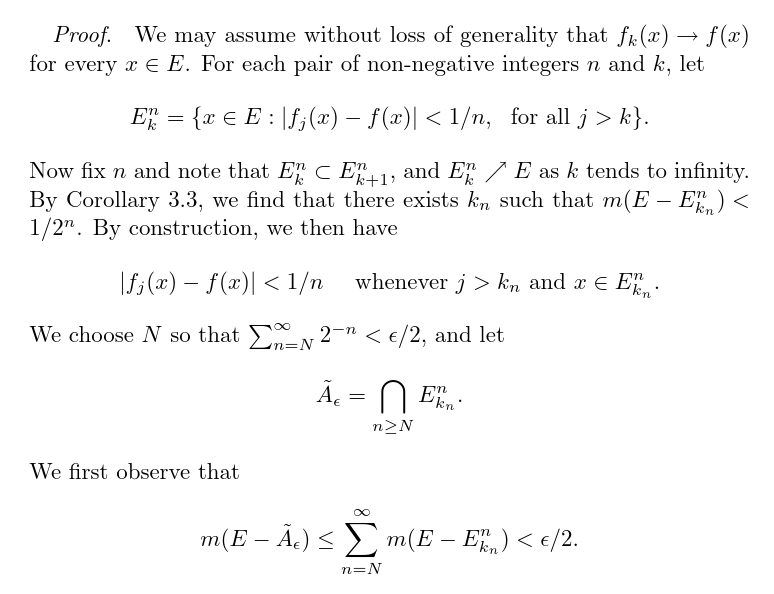
\includegraphics{figures/2021-06-11_18-07-43.png}

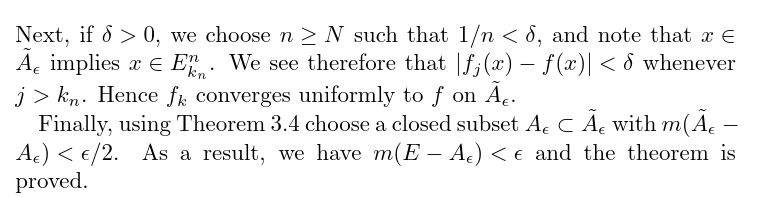
\includegraphics{figures/2021-06-11_18-07-58.png}

\end{proof}

\begin{theorem}[Lusin's Theorem]

If \(f\) is measurable and finite-valued on \(E\) with
\(\mu(E) < \infty\) then for every \({\varepsilon}>0\) there exists a
closed set \(F_{\varepsilon}\) with
\begin{align*}
F_{\varepsilon}\subset F && \mu(E - F_{\varepsilon}) \leq {\varepsilon}
\end{align*}
where \(f\) restricted to \(F_{\varepsilon}\) is continuous.

\begin{quote}
Note: this means that the separate function
\(\tilde f \coloneqq{ \left.{{f}} \right|_{{F_{\varepsilon}}} }\) is
continuous, not that the function \(f\) defined on all of \(E\) is
continuous at points of \(F_{\varepsilon}\).
\end{quote}

\end{theorem}

\begin{proof}[of Lusin]

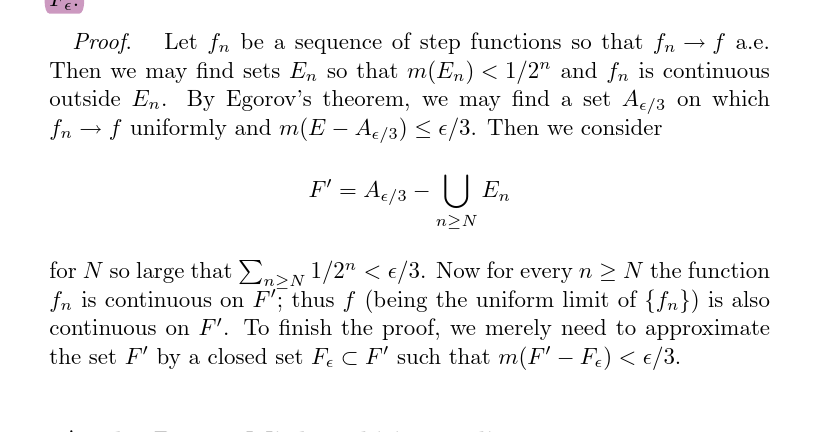
\includegraphics{figures/2021-06-11_18-04-52.png}

\end{proof}

\hypertarget{slightly-advanced-stuff}{%
\subsection{Slightly Advanced Stuff}\label{slightly-advanced-stuff}}

\begin{theorem}[Weierstrass Approximation]

If \([a, b] \subset {\mathbb{R}}\) is a closed interval and \(f\) is
continuous, then for every \({\varepsilon}> 0\) there exists a
polynomial \(p_{\varepsilon}\) such that
\({\left\lVert {f- p_{\varepsilon}} \right\rVert}_{L^\infty([a, b])} \overset{{\varepsilon}\to 0}\to 0\).

Equivalently, polynomials are dense in the Banach space
\(C([0, 1], {\left\lVert {{-}} \right\rVert}_\infty)\).

\end{theorem}

\hypertarget{examples-and-counterexamples}{%
\subsection{Examples and
Counterexamples}\label{examples-and-counterexamples}}

\begin{example}[?]

A series of continuous functions that does \emph{not} converge uniformly
but is still continuous:
\begin{align*}  
g(x) \coloneqq\sum {1 \over 1 + n^2 x}
.\end{align*}

Take \(x = 1/n^2\).

\end{example}

Let all of the following integrals to be over a compact interval
\([a, b]\) with \(0 \leq a < b\).

Questions to ask:

\begin{itemize}
\tightlist
\item
  Where is/isn't \(f\) continuous?
\item
  Where is/isn't \(f\) differentiable?
\item
  Is \(f\) Riemann integrable?
\end{itemize}

\hypertarget{dirichlet-function}{%
\subsubsection{Dirichlet function}\label{dirichlet-function}}

\begin{align*}
f ( x ) = b + (a-b)~\chi(x\in {\mathbb{Q}}) = \begin{cases}
a, & x\in {\mathbb{Q}}\\
b, & \text{else}
\end{cases}
\end{align*}
(usually take \(a=1, b=0\))

\begin{itemize}
\tightlist
\item
  Continuous nowhere
\item
  Discontinuous everywhere
\item
  Not integrable
\item
  Differentiable nowhere
\end{itemize}

\hypertarget{dirichlet-with-a-continuous-point}{%
\subsubsection{Dirichlet with a Continuous
Point}\label{dirichlet-with-a-continuous-point}}

\begin{align*}
f ( x ) = x~\chi({\mathbb{Q}}) = 
\begin{cases}
x, & x\in {\mathbb{Q}}\\
0, & \text{else}
\end{cases}
\end{align*}

\begin{itemize}
\tightlist
\item
  Continuous at 0
\item
  Discontinuous at \({\mathbb{R}}-\left\{{0}\right\}\)
\item
  Not integrable

  \begin{itemize}
  \tightlist
  \item
    \(U(f) > \frac 1 4\) but \(L(f) = 0\).
  \end{itemize}
\item
  Differentiable nowhere
\end{itemize}

\hypertarget{dirichlet-with-a-differentiable-point}{%
\subsubsection{Dirichlet with a Differentiable
Point}\label{dirichlet-with-a-differentiable-point}}

\begin{align*}
f ( x ) = x^2~\chi({\mathbb{Q}}) = \begin{cases}
x^2, & x\in {\mathbb{Q}}\\
0, & \text{else}
\end{cases}
\end{align*}

\begin{itemize}
\tightlist
\item
  Continuous at 0
\item
  Discontinuous at \({\mathbb{R}}-\left\{{0}\right\}\)
\item
  Not integrable
\item
  Differentiable at 0
\end{itemize}

\hypertarget{dirichlet-with-two-functions}{%
\subsubsection{Dirichlet with Two
Functions}\label{dirichlet-with-two-functions}}

\begin{align*}
f ( x ) = x~\chi{{\mathbb{Q}}} + (-x)\chi({\mathbb{R}}-{\mathbb{Q}}) = \begin{cases}
x, & x\in {\mathbb{Q}}\\
-x, & \text{else}
\end{cases}
\end{align*}

\begin{itemize}
\tightlist
\item
  Continuous at 0
\item
  Discontinuous at \({\mathbb{R}}-\left\{{0}\right\}\)
\item
  Differentiable nowhere.
\item
  Not integrable
\end{itemize}

\begin{proof}[of non-integrability]

Restrict attention to \({\left[ {\frac 1 2, 1} \right]}\)
\begin{align*}
\overline{\int_0^1} f 
&= \inf \left\{{ \sum \sup f(x) (x_i - x_{i-1}) }\right\} \\
\sup f(x) = x_i \implies 
\sum \sup f(x) (x_i - x_{i-1}) &= \sum x_i (x_i - x_{i-1}) \\
&> \sum \frac 1 2 (x_i - x_{i-1}) \\
&= \frac 1 2 \left(\frac 1 2\right) = \frac 1 4 \\
\implies \overline{\int_0^1} f &\geq \frac 1 4
\end{align*}
and
\begin{align*}
\underline{\int_0^1} f 
&= \sup \left\{{ \sum \inf f(x) (x_i - x_{i-1})}\right\} \\
\inf f(x)= -x_i \implies 
\sum \inf f(x) (x_i - x_{i-1}) 
&= \sum -x_i (x_i - x_{i-1}) \\
&< -\sum \frac 1 2 (x_i - x_{i-1}) \\
&= -\frac 1 2 \left( \frac 1 2 \right) = -\frac 1 4 \\
\implies \underline{\int_0^1} f &\leq -\frac 1 4
\end{align*}
So we have
\(\underline{\int_0^1} f \lneq 0 \lneq \overline{\int_0^1} f\).

\end{proof}

\hypertarget{the-thomae-function}{%
\subsection{The Thomae function:}\label{the-thomae-function}}

\begin{align*}
f ( x ) = \begin{cases}
\frac 1 q, & x = \frac p q \in {\mathbb{Q}},~(p,q) = 1 \\
0, & \text{else}
\end{cases}
\end{align*}

\begin{itemize}
\tightlist
\item
  Continuous on \({\mathbb{R}}-{\mathbb{Q}}\)
\item
  Discontinuous on \({\mathbb{Q}}\)
\item
  Integrable with \(\int_a^b f = 0\)
\item
  Differentiable nowhere
\end{itemize}

Exercises from Folland:

\begin{itemize}
\item
  Chapter 1: Exercises 3, 7, 10, 12, 14 (with the sets in 3(a) being
  non-empty) Exercises 15, 17, 18, 19, 22(a), 24, 28 Exercises 26, 30
  (also check out 31)
\item
  Chapter 2: Exercises 2, 3, 7, 9 (in 9(c) you can use Exercise 1.29
  without proof Exercises 10, 12, 13, 14, 16, 19 Exercises 24, 25,
  28(a,b), 33, 34, 35, 38, 41 (note that 24 shows that upper sums are
  not needed in the definition of integrals, and the extra hypotheses
  also show that they are not desired either) Exercises 40, 44, 47, 49,
  50, 51, 52, 54, 56, 58, 59
\item
  Chapter 3: Exercises 3(b,c), 5, 6, 9, 12, 13, 14, 16, 20, 21, 22
\end{itemize}

\hypertarget{measure-theory}{%
\section{Measure Theory}\label{measure-theory}}

\begin{fact}

Some useful tricks:

\begin{itemize}
\tightlist
\item
  \(\mu(A\setminus B) = \mu(A) - \mu(B)\) if \(\mu(B) < \infty\)
\item
  Write \(f = f-f_n + f_n\)
\item
  If \(G\) is measurable, then there exists an \(E \supseteq G\) such
  \(m(G) \leq m(E) + {\varepsilon}\)
\item
  If \(E\) is measurable,

  \begin{itemize}
  \tightlist
  \item
    \(E = F_{\delta} {\textstyle\coprod}N\) for \(N\) a null set.
  \item
    \(E {\textstyle\coprod}N = G_{\delta}\) for \(N\) a null set.
  \end{itemize}
\end{itemize}

\end{fact}

\hypertarget{abstract-measure-theory}{%
\subsection{Abstract Measure Theory}\label{abstract-measure-theory}}

\begin{definition}[Measures on measurable spaces]

If \((X, {\mathcal{M}})\) is a measurable space, then a \textbf{measure}
is a function \(\mu: {\mathcal{M}}\to [0,\infty]\) such that

\begin{enumerate}
\def\labelenumi{\arabic{enumi}.}
\tightlist
\item
  \(\mu(\emptyset) = 0\).
\item
  Countable additivity: if \(\left\{{E_k}\right\}_{k\geq 1}\) is a
  countable union of disjoint sets in \(X\), then
  \begin{align*}
  \mu\qty{{\textstyle\coprod}_{k\geq 1} E_k} = \sum_{k\geq 1} \mu(E_k)
  .\end{align*}
\end{enumerate}

If (2) only holds for finitely indexed sums, we say \(\mu\) is
\textbf{\(\sigma{\hbox{-}}\)additive}.

\end{definition}

\begin{proposition}[Subtraction of Measures]

\begin{align*}m(A) = m(B) + m(C) {\quad \operatorname{and} \quad} m(C) < \infty \implies m(A) - m(C) = m(B).\end{align*}

\end{proposition}

\begin{theorem}[Properties of measures]

Let \((X, {\mathcal{M}}, \mu)\) be a measure space. Then

\begin{enumerate}
\def\labelenumi{\arabic{enumi}.}
\tightlist
\item
  Monotonicity: \(E \subseteq F \implies \mu(E) \leq \mu(F)\).
\item
  Countable subadditivity: If \(ts{E_k}_{k\geq 1}\) is a countable
  collection,
  \begin{align*}
  \mu\qty{\displaystyle\bigcup_{k\geq 1} E_k} \leq \sum_{k\geq 1} \mu(E_k)
  .\end{align*}
\end{enumerate}

\end{theorem}

\begin{proposition}[Continuity of Measure]

\begin{align*}
\text{Continuity from below:} \quad 
E_{n} \nearrow E &\implies m(E_{n}) \to m(E) \\
\text{Continuity from above:} \quad 
m(E_{1}) < \infty \text{ and } E_{i} \searrow E &\implies m(E_{i}) \to m(E)
.\end{align*}

Mnemonic: \(\lim_n \mu(E_n) = \mu(\lim E_n)\).

\end{proposition}

\begin{proof}[sketches]

\envlist

\begin{itemize}
\tightlist
\item
  From below: break into disjoint annuli
  \(A_{2} = E_{2}\setminus E_{1}\),

  \begin{itemize}
  \tightlist
  \item
    Apply countable disjoint additivity to
    \(E = {\textstyle\coprod}A_{i}\).
  \end{itemize}
\item
  From above: funny step, use
  \(E_{1} = ({\textstyle\coprod}E_{j}\setminus E_{j+1}) {\textstyle\coprod}(\cap E_{j})\).

  \begin{itemize}
  \tightlist
  \item
    Taking measures yields a telescoping sum, and use countable
    additivity, then finiteness to subtract.
  \end{itemize}
\end{itemize}

\begin{figure}
\centering
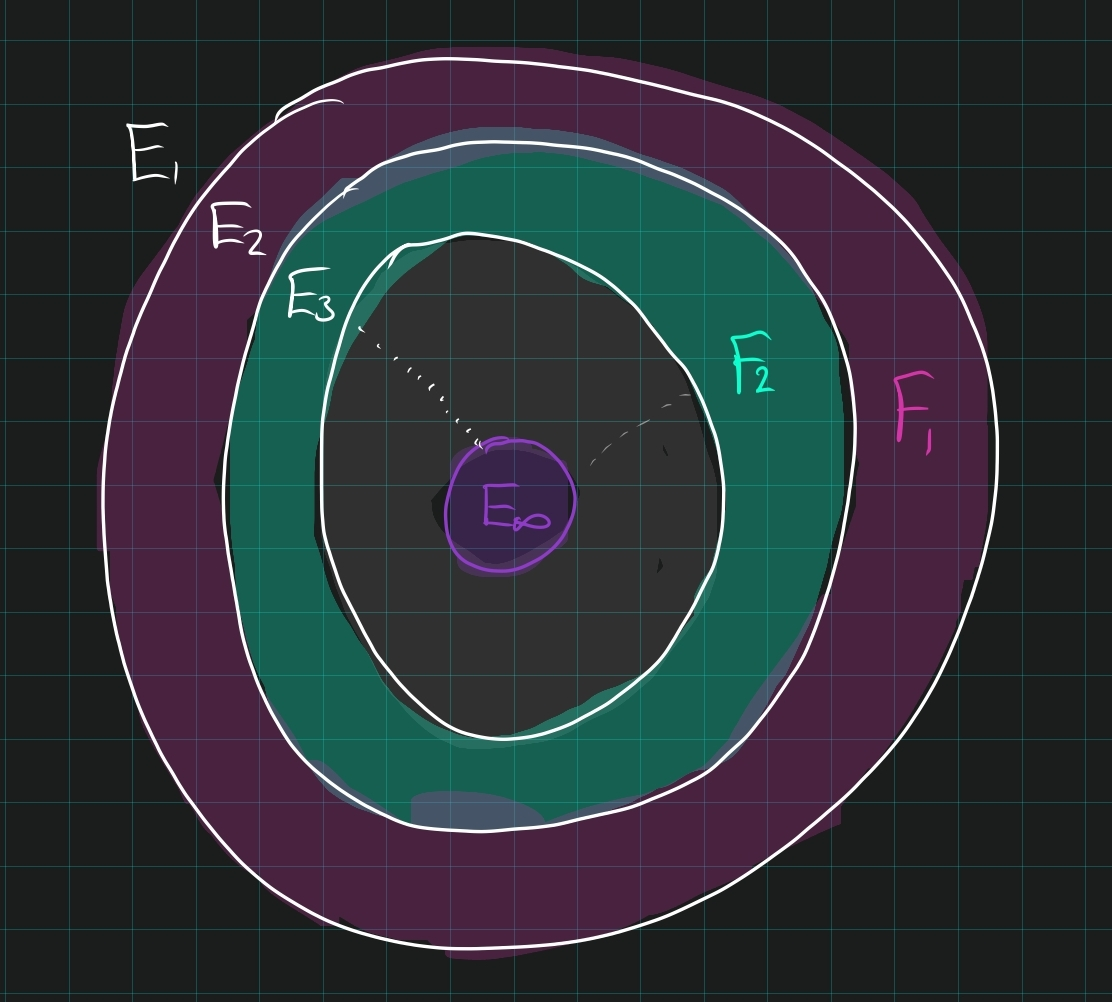
\includegraphics{figures/image_2021-05-28-23-29-31.png}
\caption{image\_2021-05-28-23-29-31}
\end{figure}

\end{proof}

\begin{proof}[of continuity of measure from below, detailed]

For any measure \(\mu\),
\begin{align*}
\mu(F_1) < \infty,\, F_k \searrow F \implies \lim_{k\to\infty}\mu(F_k) = \mu(F)
,\end{align*}
where \(F_k \searrow F\) means \(F_1 \supseteq F_2 \supseteq \cdots\)
with \(\cap_{k=1}^\infty F_k = F\). - Note that \(\mu(F)\) makes sense:
each \(F_k \in \mathcal{B}\), which is a \(\sigma{\hbox{-}}\)algebra and
closed under countable intersections.

\begin{itemize}
\item
  Take disjoint annuli by setting
  \(E_k \coloneqq F_k \setminus F_{k+1}\)
\item
  Funny step: write
  \begin{align*}
  F_1 = F {\textstyle\coprod}\displaystyle\coprod_{k=1}^{\infty} E_k
  .\end{align*}

  \begin{itemize}
  \tightlist
  \item
    This is because \(x\in F_1\) iff \(x\) is in every \(F_k\), so in
    \(F\), \textbf{or}
  \item
    \(x\not \in F_1\) but \(x\in F_2\), noting incidentally
    \(x\in F_3, F_4,\cdots\), \textbf{or},
  \item
    \(x\not\in F_2\) but \(x\in F_3\), and so on.
  \end{itemize}
\item
  Now take measures, and note that we get a telescoping sum:
  \begin{align*}
  \mu(F_1) 
  &= \mu(F) + \sum_{k=1}^\infty \mu(E_k) \\
  &= \mu(F) + \lim_{N\to\infty} \sum_{k=1}^N \mu(E_k) \\
  &\coloneqq\mu(F) + \lim_{N\to\infty} \sum_{k=1}^N \mu(F_k \setminus F_{k+1} ) \\
  &\coloneqq\mu(F) + \lim_{N\to\infty} \sum_{k=1}^N \mu(F_k) - \mu(F_{k+1} ) \hspace{5em}\text{to be justified}\\
  &= \mu(F) + \lim_{N\to\infty} 
  [
  (\mu(F_1) - \mu(F_2)) +  
  (\mu(F_2) - \mu(F_3)) +  
  \cdots \\ 
  & \hspace{8em} + (\mu(F_{N-1}) - \mu(F_N)) +  
  (\mu(F_N) - \mu(F_{N+1})) 
  ] \\ \\
  &= \mu(F) + \lim_{N\to\infty} \mu(F_1) - \mu(F_{N+1}) \\
  &= \mu(F) + \mu(F_1) - \lim_{N\to\infty} \mu(F_{N+1})
  .\end{align*}
\item
  Justifying the measure subtraction: the general statement is that for
  any pair of sets \(A\subseteq X\),
  \(\mu(X\setminus A) = \mu(X) - \mu(A)\) when \(\mu(A) < \infty\):
  \begin{align*}
  X &= A {\textstyle\coprod}(X\setminus A) \\
  \implies \mu(X) &= \mu(A) + \mu(X\setminus A) && \text{countable additivity} \\
  \implies \mu(X) -\mu(A) &= \mu(X\setminus A) && \text{if } \mu(A) < \infty 
  .\end{align*}
\item
  Now use that \(\mu(F_1)<\infty\) to justify subtracting it from both
  sides:
  \begin{align*}
  \mu(F_1)
  &= \mu(F) + \mu(F_1) - \lim_{N\to\infty} \mu(F_{N+1}) \\
  \implies
  0
  &= \mu(F_1) - \lim_{N\to\infty} \mu(F_{N+1}) \\
  \lim_{N\to\infty} \mu(F_{N+1})
  &= \mu(F_1) 
  .\end{align*}
\item
  Now use that
  \(\lim_{N\to\infty}\mu(F_{N+1}) = \lim_{N\to\infty} \mu(F_N)\) to
  conclude.
\end{itemize}

\end{proof}

\hypertarget{outer-measure}{%
\subsection{Outer Measure}\label{outer-measure}}

\begin{proposition}[Properties of Outer Measure]

\envlist

\begin{enumerate}
\def\labelenumi{\arabic{enumi}.}
\tightlist
\item
  Monotonicity: \(E\subseteq F \implies m_*(E) \leq m_*(F)\).
\item
  Countable Subadditivity: \(m_*(\cup E_{i}) \leq \sum m_*(E_{i})\).
\item
  Approximation: For all \(E\) there exists a \(G \supseteq E\) such
  that \(m_*(G) \leq m_*(E) + \varepsilon\).
\item
  Disjoint\footnote{This holds for outer measure \textbf{iff}
    \(\mathrm{dist}(A, B) > 0\).} Additivity:
  \(m_*(A {\textstyle\coprod}B) = m_*(A) + m_*(B)\).
\end{enumerate}

\end{proposition}

\hypertarget{measures-on-mathbbrd}{%
\subsection{\texorpdfstring{Measures on
\({\mathbb{R}}^d\)}{Measures on \{\textbackslash mathbb\{R\}\}\^{}d}}\label{measures-on-mathbbrd}}

\begin{proposition}[Borel Characterization of Measurable Sets]

If \(E\) is Lebesgue measurable, then \(E = H {\textstyle\coprod}N\)
where \(H \in F_\sigma\) and \(N\) is null.

\end{proposition}

\begin{proposition}[Opens are unions of almost disjoint intervals.]

Every open subset of \({\mathbb{R}}\) (resp \({\mathbb{R}}^n\)) can be
written as a unique countable union of disjoint (resp. almost disjoint)
intervals (resp. cubes).

\end{proposition}

\begin{theorem}[Measurable sets can be approximated by open/closed/compact sets.]

Suppose \(E\) is measurable; then for every \({\varepsilon}>0\),

\begin{enumerate}
\def\labelenumi{\arabic{enumi}.}
\tightlist
\item
  There exists an open \(O\supset E\) with
  \(m(O\setminus E) < {\varepsilon}\)
\item
  There exists a closed \(F\subset E\) with
  \(m(E\setminus F) < {\varepsilon}\)
\item
  There exists a compact \(K\subset E\) with
  \(m(E\setminus K) < {\varepsilon}\).
\end{enumerate}

\end{theorem}

\begin{proof}[that measurable sets can be approximated]

\envlist

\begin{itemize}
\tightlist
\item
  (1): Take \(\left\{{Q_{i}}\right\} \rightrightarrows E\) and set
  \(O = \cup Q_{i}\).
\item
  (2): Since \(E^c\) is measurable, produce \(O\supset E^c\) with
  \(m(O\setminus E^c) < {\varepsilon}\).

  \begin{itemize}
  \tightlist
  \item
    Set \(F = O^c\), so \(F\) is closed.
  \item
    Then \(F\subset E\) by taking complements of \(O\supset E^c\)
  \item
    \(E\setminus F = O\setminus E^c\) and taking measures yields
    \(m(E\setminus F) < {\varepsilon}\)
  \end{itemize}
\item
  (3): Pick \(F\subset E\) with \(m(E\setminus F) < {\varepsilon}/2\).

  \begin{itemize}
  \tightlist
  \item
    Set \(K_{n} = F\cap{\mathbb{D}}_{n}\), a ball of radius \(n\) about
    \(0\).
  \item
    Then \(E\setminus K_{n} \searrow E\setminus F\)
  \item
    Since \(m(E) < \infty\), there is an \(N\) such that
    \(n\geq N \implies m(E\setminus K_{n}) < {\varepsilon}\).
  \end{itemize}
\end{itemize}

\end{proof}

\begin{proposition}[Translation and Dilation Invariance]

Lebesgue measure is translation and dilation invariant.

\end{proposition}

\begin{proof}[(Todo) of translation/dilation invariance]

Obvious for cubes; if \(Q_{i} \rightrightarrows E\) then
\(Q_{i} + k \rightrightarrows E + k\), etc.

\end{proof}

\begin{theorem}[Non-measurable sets exist]

There is a non-measurable set \(A\subseteq {\mathbb{R}}\).

\end{theorem}

\begin{proof}[Constructing a non-measurable set]

\envlist

\begin{itemize}
\tightlist
\item
  Use AOC to choose one representative from every coset of
  \({\mathbb{R}}/{\mathbb{Q}}\) on \([0, 1)\), which is countable, and
  assemble them into a set \(N\)
\item
  Enumerate the rationals in \([0, 1]\) as \(q_{j}\), and define
  \(N_{j} = N + q_{j}\). These intersect trivially.
\item
  Define \(M \coloneqq{\textstyle\coprod}N_{j}\), then
  \([0, 1) \subseteq M \subseteq [-1, 2)\), so the measure must be
  between 1 and 3.
\item
  By translation invariance, \(m(N_{j}) = m(N)\), and disjoint
  additivity forces \(m(M) = 0\), a contradiction.
\end{itemize}

\end{proof}

\begin{proof}[of Borel characterization]

For every \(\frac 1 n\) there exists a closed set \(K_{n} \subset E\)
such that \(m(E\setminus K_{n}) \leq \frac 1 n\). Take
\(K = \cup K_{n}\), wlog \(K_{n} \nearrow K\) so
\(m(K) = \lim m(K_{n}) = m(E)\). Take \(N\coloneqq E\setminus K\), then
\(m(N) = 0\).

\end{proof}

\begin{proposition}[Limsups/infs of measurable sets are measurable.]

If \(A_{n}\) are all measurable, \(\limsup A_{n}\) and \(\liminf A_{n}\)
are measurable.

\end{proposition}

\begin{proof}[That limsups/infs are measurable]

Measurable sets form a sigma algebra, and these are expressed as
countable unions/intersections of measurable sets.

\end{proof}

\begin{theorem}[Borel-Cantelli]

Let \(\{E_{k}\}\) be a countable collection of measurable sets. Then
\begin{align*}
\sum_{k} m(E_{k}) < \infty \implies \text{ almost every } x\in {\mathbb{R}}\text{ is in at most finitely many } E_{k}
.\end{align*}

\end{theorem}

\begin{proof}[of Borel-Cantelli]

\envlist

\begin{itemize}
\tightlist
\item
  If \(E = \limsup_{j} E_{j}\) with \(\sum m(E_{j}) < \infty\) then
  \(m(E) = 0\).
\item
  If \(E_{j}\) are measurable, then \(\limsup_{j} E_{j}\) is measurable.
\item
  If \(\sum_{j} m(E_{j}) < \infty\), then
  \(\sum_{j=N}^\infty m(E_{j}) \overset{N\to\infty}\to 0\) as the tail
  of a convergent sequence.
\item
  \(E = \limsup_{j} E_{j} = \cap_{k=1}^\infty \cup_{j=k}^\infty E_{j} \implies E \subseteq \cup_{j=k}^\infty\)
  for all \(k\)
\item
  \(E \subset \cup_{j=k}^\infty \implies m(E) \leq \sum_{j=k}^\infty m(E_{j}) \overset{k\to\infty}\to 0\).
\end{itemize}

\end{proof}

\begin{proposition}[Extending the class of measurable functions.]

\begin{itemize}
\tightlist
\item
  Characteristic functions are measurable
\item
  If \(f_{n}\) are measurable, so are
  \({\left\lvert {f_{n}} \right\rvert}, \limsup f_{n}, \liminf f_{n}, \lim f_{n}\),
\item
  Sums and differences of measurable functions are measurable,
\item
  Cones \(F(x,y) = f(x)\) are measurable,
\item
  Compositions \(f\circ T\) for \(T\) a linear transformation are
  measurable,
\item
  ``Convolution-ish'' transformations \((x,y) \mapsto f(x-y)\) are
  measurable
\end{itemize}

\end{proposition}

\begin{proof}[Convolution]

Take the cone on \(f\) to get \(F(x, y) = f(x)\), then compose \(F\)
with the linear transformation \(T = [1, -1; 1, 0]\).

\end{proof}

\begin{definition}[$\sigma\dash$finiteness]

A measure space \((X, {\mathcal{M}}, \mu)\) is
\textbf{\(\sigma{\hbox{-}}\)finite} if \(X\) can be written as a union
of countably many measurable sets with finite measure.

\end{definition}

\begin{proposition}[Regularity of measure]

If \((X, {\mathcal{B}}, \mu)\) is a Borel measure space where \(\mu\) is
finite on all balls of finite radius, then for any
\(E \in {\mathcal{B}}\) and any \({\varepsilon}>0\),

\begin{itemize}
\tightlist
\item
  There exists an open set \(O\) with \(E \subset O\) and
  \(\mu(O\setminus E) < {\varepsilon}\)
\item
  There exists a closed set \(F\) with \(F\subset E\) and
  \(\mu(E\setminus F) < {\varepsilon}\).
\end{itemize}

\end{proposition}

\begin{problem}[?]

Show that \(E\) is measurable iff \(E\) is regular in either sense
above.

\end{problem}

\hypertarget{exercises}{%
\subsection{Exercises}\label{exercises}}

\begin{problem}[?]

Show that if \(\sum \mu(E_k) < \infty\) then almost every \(x\in X\) is
in at most finitely many \(E_k\).

\end{problem}

\hypertarget{integration}{%
\section{Integration}\label{integration}}

\hypertarget{unsorted}{%
\subsection{Unsorted}\label{unsorted}}

\begin{definition}[Measurable Function]

A function \(f: (X, {\mathcal{M}}_X) \to (Y, {\mathcal{M}}_Y)\) is
\textbf{\(({\mathcal{M}}_X, {\mathcal{M}}_Y){\hbox{-}}\)measurable} iff
\(f^{-1}({\mathcal{M}}_Y) \subseteq {\mathcal{M}}_X\). Equivalently, if
\({\mathcal{E}}_Y\) is a generating set for \({\mathcal{B}}_Y\),
\(f^{-1}({\mathcal{E}}_Y) \subseteq {\mathcal{B}}_X\).

\begin{itemize}
\tightlist
\item
  An functional on a general measurable space
  \(f: f:(X, {\mathcal{M}}_X) \to ({\mathbb{R}}, {\mathcal{B}}_{\mathbb{R}})\)
  is \textbf{measurable} \(\iff f\) is
  \(({\mathcal{M}}_X, {\mathcal{B}}_{\mathbb{R}}){\hbox{-}}\)measurable.
\item
  A functional \(f: {\mathbb{R}}^d\to {\mathbb{R}}\) is \textbf{Borel
  measurable} iff \(f\) is
  \(({\mathcal{B}}_{{\mathbb{R}}^d}, {\mathcal{B}}_{\mathbb{R}}){\hbox{-}}\)measurable.
\item
  A functional \(f: {\mathbb{R}}^d\to {\mathbb{R}}\) is \textbf{Lebesgue
  measurable} iff \(f\) is
  \(({\mathcal{L}}_{{\mathbb{R}}^d}, {\mathcal{B}}_{\mathbb{R}}){\hbox{-}}\)measurable.
\end{itemize}

Using that \({\mathcal{B}}_{{\mathbb{R}}}\) is generated by open/closed
rays, it suffices to check any of the following (for all
\(\alpha \in {\mathbb{R}}\)):

\begin{itemize}
\tightlist
\item
  \(f^{-1}(\alpha, \infty)\in {\mathcal{M}}\)
\item
  \(f^{-1}[\alpha, \infty)\in {\mathcal{M}}\)
\item
  \(f^{-1}(-\infty, \alpha)\in {\mathcal{M}}\)
\item
  \(f^{-1}(-\infty, \alpha]\in {\mathcal{M}}\)
\end{itemize}

\end{definition}

\begin{remark}

Note that we still require Borel sets in the target for Lebesgue
measurability! Taking
\(({\mathcal{L}}_{{\mathbb{R}}^d}, {\mathcal{L}}_{\mathbb{R}})\)
functions is too stringent, e.g.~this class does not contain continuous
functionals.

\end{remark}

\begin{warnings}

If \(f\) is \({\mathcal{L}}{\hbox{-}}\)measurable and \(h\) is
continuous, it's not necessarily true that \(k\coloneqq f\circ h\) is
\({\mathcal{L}}{\hbox{-}}\)measurable. Standard counterexample: set
\(g(x) \coloneqq C(x) + x\) for \(C\) the Cantor-Lebesgue function, then
\(g:[0, 1]\to [0, 2]\) is a homeomorphism. Then \(m(g(C)) = 1\) since
\(f\) is constant on intervals in \(C^c\), so use Vitali's theorem: a
set is null iff every subset is measurable. So \(g(C)\) contains a
non-measurable set \(A\). Define \(B\coloneqq g^{-1}(A)\), then
\(B \subset C\) and \(m(C) = 0\) implies \(B\) is measurable and
\(\chi_B\) is a measurable function. But then
\(k\coloneqq\chi_B \circ g^{-1}\) is not
\({\mathcal{L}}{\hbox{-}}\)measurable, since \(k^{-1}(1) = A\) is a
non-measurable set, but \(\chi_B\) is
\({\mathcal{L}}{\hbox{-}}\)measurable and \(g^{-1}\) is continuous.

\end{warnings}

\begin{proposition}[Closure of measurable functions under operations]

\({\mathcal{M}}{\hbox{-}}\)measurable functionals are closed under

\begin{itemize}
\tightlist
\item
  Sums
\item
  Products
\item
  Sups/infs
\item
  Limsups/Liminfs
\item
  Limits when they exist, and the limiting function is measurable.
\item
  \(\max(f, g)\) and \(\min(f, g)\).
\end{itemize}

Characteristic functions on measurable sets are automatically
measurable, since
\(E\in {\mathcal{M}}\implies E = \chi_E^{-1}(\left\{{1}\right\})\).

\end{proposition}

\begin{remark}[A common proof technique]

\envlist

\begin{itemize}
\tightlist
\item
  Show something holds for indicator functions.
\item
  Show it holds for simple functions by linearity.
\item
  Use \(s_k \nearrow f\) and apply MCT to show it holds for \(f\).
\end{itemize}

\end{remark}

\begin{remark}[on notation]

\envlist

\begin{itemize}
\tightlist
\item
  \(L^+\): measurable functions
\item
  \(L^1\): Lebesgue integrable functions, so
  \(\int {\left\lvert {f} \right\rvert} < \infty\)
\end{itemize}

\end{remark}

\begin{definition}[Simple Function]

A \textbf{simple function} \(s: {\mathbb{C}}\to X\) is a finite linear
combination of indicator functions of measurable sets, i.e.~
\begin{align*}
s(x) = \sum_{j=1}^n c_j \chi_{E_j}(x)
.\end{align*}

\end{definition}

\begin{definition}[Lebesgue Integral]

\begin{align*}
\int_X f \coloneqq\sup \left\{{ \int s(x) \,d\mu{~\mathrel{\Big|}~}0\leq s \leq f, s\text{ simple } }\right\} 
.\end{align*}

Note that if \(s = \sum c_j \chi_{E_j}\) is simple, then
\begin{align*}
\int_X s(x) \,d\mu\coloneqq\sum_{j=1}^n c_j \mu(E_j)
.\end{align*}

\end{definition}

\begin{remark}[Integrals split across disjoint sets]

A useful fact: for \((X, \mathcal{M})\) a measure space, integrals split
across disjoint sets:
\begin{align*}
\int_X f = \int_{X\setminus A} f + \int_A f && \forall\, A \in \mathcal{M} 
.\end{align*}

\end{remark}

\begin{definition}[Essential supremum and infimum, essentially bounded]

An \textbf{essential lower bound} \(b\) on a function \(f\) is any real
number such that
\(S_{b} \coloneqq\left\{{x{~\mathrel{\Big|}~}f(x) < b }\right\} = f^{-1}(-\infty, b)\)
has measure zero. The \textbf{essential infimum} is the supremum of all
essential lower bounds,
i.e.~\({\mathrm{ess}}\inf f \coloneqq\sup_{b} \left\{{b{~\mathrel{\Big|}~}\mu S_b = 0}\right\}\).
This is the greatest lower bound almost everywhere.

Similarly an \textbf{essential upper bound} \(c\) is any number such
that \(S^c \coloneqq f^{-1}(c, \infty)\) has measure zero, and the
\textbf{essential supremum} is
\({\mathrm{ess}}\sup f \coloneqq\inf_{c} \left\{{c{~\mathrel{\Big|}~}\mu S^c = 0}\right\}\),
which is the least upper bound almost everywhere.

A function is \textbf{essentially bounded} if
\({\left\lVert {f} \right\rVert}_\infty \coloneqq{\mathrm{ess}}\sup f < \infty\).
These are functions which are bounded almost everywhere.

\end{definition}

\begin{example}[An essentially bounded but not bounded function]

\(f(x) = x\chi_{\mathbb{Q}}(x)\) is essentially bounded but not bounded.

\end{example}

\begin{proposition}[$L^\infty$ functions are equivalent to bounded almost-everywhere functions]

If \(f\in L^\infty(X)\), then \(f\) is equal to some bounded function
\(g\) almost everywhere.

\end{proposition}

\begin{theorem}[p-Test for Integrals]

\begin{align*}
\int_0^1 {1\over x^p} < \infty \iff  p < 1 \\
\int_1^\infty {1\over x^p} < \infty \iff  p > 1 
.\end{align*}

\end{theorem}

\begin{slogan}

Large powers of \(x\) help us in neighborhoods of infinity and hurt
around zero.

\end{slogan}

\begin{theorem}[Monotone Convergence]

If \(f_n: X\to [0, \infty) \in L^+\) and \(f_n \nearrow f\) almost
everywhere, then
\begin{align*}
\lim \int f_n
= \int \lim f_n = \int f
\quad \text{i.e.}~~ \int f_n \to \int f
.\end{align*}

\end{theorem}

\begin{slogan}

Measurable, non-negative, increasing pointwise a.e. allows commuting
limits and integrals.

\end{slogan}

\begin{proof}[of MCT]

\todo[inline]{todo}

\end{proof}

\begin{theorem}[Dominated Convergence]

If \(f_n \in L^1\) and \(f_n \to f\) almost everywhere with
\({\left\lvert {f_n} \right\rvert} \leq g\) for some \(g\in L^1\), then
\(f\in L^1\) and
\begin{align*}
\int {\left\lvert {f_n - f} \right\rvert} \to 0
.\end{align*}

As a consequence,
\begin{align*}
\lim \int f_n = \int \lim f_n = \int f \quad \text{i.e.}~~ \int f_n \to \int f < \infty
\end{align*}

\begin{quote}
Positivity \emph{not} needed.
\end{quote}

\end{theorem}

\begin{proof}[of DCT]

\todo[inline]{todo}

\end{proof}

\begin{theorem}[Generalized DCT]

If

\begin{itemize}
\tightlist
\item
  \(f_n \in L^1\) with \(f_n \to f\) almost everywhere,
\item
  There exist \(g_n \in L^1\) with
  \({\left\lvert {f_n} \right\rvert} \leq g_n\), \(g_n \geq 0\).
\item
  \(g_n\to g\) almost everywhere with \(g\in L^1\), and
\item
  \(\lim \int g_n = \int g\),
\end{itemize}

then \(f\in L^1\) and \(\lim \int f_n = \int f < \infty\).

\begin{quote}
Note that this is the DCT with
\({\left\lvert {f_n} \right\rvert} < {\left\lvert {g} \right\rvert}\)
relaxed to \({\left\lvert {f_n} \right\rvert} < g_n \to g\in L^1\).
\end{quote}

\end{theorem}

\begin{proof}

Proceed by showing
\(\limsup \int f_n \leq \int f \leq \liminf \int f_n\):

\begin{itemize}
\item
  \(\int f \geq \limsup \int f_n\):
  \begin{align*}
  \int g - \int f 
  &= \int \qty{g-f} \\
  &\leq \liminf \int \qty{g_n - f_n} \quad \text{Fatou} \\
  &= \lim \int g_n + \liminf \int (-f_n) \\
  &= \lim \int g_n - \limsup \int f_n \\
  &= \int g - \limsup \int f_n \\
  \\
  \implies \int f &\geq \limsup \int f_n
  .\end{align*}

  \begin{itemize}
  \tightlist
  \item
    Here we use \(g_n - f_n \overset{n\to\infty} g-f\) with
    \(0 \leq {\left\lvert {f_n} \right\rvert} - f_n \leq g_n - f_n\), so
    \(g_n - f_n\) are nonnegative (and measurable) and Fatou's lemma
    applies.
  \end{itemize}
\item
  \(\int f \leq \liminf \int f_n\):
  \begin{align*}
  \int g + \int f 
  &= \int(g+f) \\
  &\leq \liminf \int \qty{g_n + f_n} \\
  &= \lim \int g_n + \liminf \int f_n \\
  &= \int g + \liminf f_n \\
  \\
  \int f &\leq \liminf \int f_n
  .\end{align*}

  \begin{itemize}
  \tightlist
  \item
    Here we use that \(g_n + f_n \to g+f\) with
    \(0 \leq {\left\lvert {f_n} \right\rvert} + f_n \leq g_n + f_n\) so
    Fatou's lemma again applies.
  \end{itemize}
\end{itemize}

\end{proof}

\begin{proposition}[Convergence in $L^1$ implies convergence of $L^1$ norm]

If \(f\in L^1\), then
\begin{align*}
\int{\left\lvert {f_n - f} \right\rvert} \to 0 \iff \int {\left\lvert {f_n} \right\rvert} \to \int {\left\lvert {f} \right\rvert}
.\end{align*}

\end{proposition}

\begin{proof}

Let
\(g_n = {\left\lvert {f_n} \right\rvert} - {\left\lvert {f_n - f} \right\rvert}\),
then \(g_n \to {\left\lvert {f} \right\rvert}\) and
\begin{align*}
{\left\lvert {g_n} \right\rvert} = {\left\lvert { {\left\lvert {f_n} \right\rvert} - {\left\lvert {f_n - f} \right\rvert} } \right\rvert} \leq {\left\lvert {f_n - (f_n - f)} \right\rvert} = {\left\lvert {f} \right\rvert} \in L^1
,\end{align*}
so the DCT applies to \(g_n\) and
\begin{align*}
{\left\lVert {f_n - f} \right\rVert}_1 = \int {\left\lvert {f_n - f} \right\rvert} + {\left\lvert {f_n} \right\rvert} - {\left\lvert {f_n} \right\rvert}
= \int {\left\lvert {f_n} \right\rvert} - g_n\\
\to_{DCT} \lim \int {\left\lvert {f_n} \right\rvert} - \int {\left\lvert {f} \right\rvert}
.\end{align*}

\end{proof}

\begin{theorem}[Fatou]

If \(f_n\) is a sequence of nonnegative measurable functions, then
\begin{align*}
\liminf_n \int f_n 
&\geq \int \liminf_n f_n \\
\limsup_n \int f_n &\leq \int \limsup_n f_n
.\end{align*}

\end{theorem}

\begin{proof}[of Fatou]

\todo[inline]{Prove Fatou}

\end{proof}

\begin{theorem}[Tonelli (Non-Negative, Measurable)]

For \(f(x, y)\) \textbf{non-negative and measurable}, for almost every
\(x\in {\mathbb{R}}^n\),

\begin{itemize}
\tightlist
\item
  \(f_x(y)\) is a \textbf{measurable} function
\item
  \(F(x) = \int f(x, y) ~dy\) is a \textbf{measurable} function,
\item
  For \(E\) measurable, the slices
  \(E_x \coloneqq\left\{{y {~\mathrel{\Big|}~}(x, y) \in E}\right\}\)
  are measurable.
\item
  \(\int f = \int \int F\), i.e.~any iterated integral is equal to the
  original.
\end{itemize}

\end{theorem}

\begin{theorem}[Fubini (Integrable)]

For \(f(x, y)\) \textbf{integrable}, for almost every
\(x\in {\mathbb{R}}^n\),

\begin{itemize}
\tightlist
\item
  \(f_x(y)\) is an \textbf{integrable} function
\item
  \(F(x) \coloneqq\int f(x, y) ~dy\) is an \textbf{integrable} function,
\item
  For \(E\) measurable, the slices
  \(E_x \coloneqq\left\{{y {~\mathrel{\Big|}~}(x, y) \in E}\right\}\)
  are measurable.
\item
  \(\int f = \int \int f(x,y)\), i.e.~any iterated integral is equal to
  the original
\end{itemize}

\end{theorem}

\begin{theorem}[Fubini-Tonelli]

If any iterated integral is \textbf{absolutely integrable},
i.e.~\(\int \int {\left\lvert {f(x, y)} \right\rvert} < \infty\), then
\(f\) is integrable and \(\int f\) equals any iterated integral.

\end{theorem}

\begin{proposition}[Measurable Slices]

Let \(E\) be a measurable subset of \({\mathbb{R}}^n\). Then

\begin{itemize}
\tightlist
\item
  For almost every \(x\in {\mathbb{R}}^{n_1}\), the slice
  \(E_x \coloneqq\left\{{y \in {\mathbb{R}}^{n_2} \mathrel{\Big|}(x,y) \in E}\right\}\)
  is measurable in \({\mathbb{R}}^{n_2}\).
\item
  The function
\end{itemize}

\begin{align*}
F: {\mathbb{R}}^{n_1} &\to {\mathbb{R}}\\
x &\mapsto m(E_x) = \int_{{\mathbb{R}}^{n_2}} \chi_{E_x} ~dy
\end{align*}
is measurable and
\begin{align*}
m(E) = \int_{{\mathbb{R}}^{n_1}} m(E_x) ~dx 
= \int_{{\mathbb{R}}^{n_1}} \int_{{\mathbb{R}}^{n_2}} \chi_{E_x} ~dy ~dx
.\end{align*}

\end{proposition}

\begin{proof}[of measurable slices]

\envlist

\(\implies\):

\begin{itemize}
\tightlist
\item
  Let \(f\) be measurable on \({\mathbb{R}}^n\).
\item
  Then the cylinders \(F(x, y) = f(x)\) and \(G(x, y) = f(y)\) are both
  measurable on \({\mathbb{R}}^{n+1}\).
\item
  Write
  \(\mathcal{A} = \left\{{G \leq F}\right\} \cap\left\{{G \geq 0}\right\}\);
  both are measurable.
\end{itemize}

\(\impliedby\):

\begin{itemize}
\tightlist
\item
  Let \(A\) be measurable in \({\mathbb{R}}^{n+1}\).
\item
  Define
  \(A_x = \left\{{y\in {\mathbb{R}}\mathrel{\Big|}(x, y) \in \mathcal{A}}\right\}\),
  then \(m(A_x) = f(x)\).
\item
  By the corollary, \(A_x\) is measurable set, \(x \mapsto A_x\) is a
  measurable function, and \(m(A) = \int f(x) ~dx\).
\item
  Then explicitly, \(f(x) = \chi_{A}\), which makes \(f\) a measurable
  function.
\end{itemize}

\end{proof}

\begin{proposition}[Differentiating Under an Integral]

If
\({\left\lvert {{\frac{\partial }{\partial t}\,}f(x, t)} \right\rvert} \leq g(x) \in L^1\),
then letting \(F(t) = \int f(x, t) ~dt\),
\begin{align*}
{\frac{\partial }{\partial t}\,} F(t)
&\coloneqq\lim_{h \rightarrow 0} \int \frac{f(x, t+h)-f(x, t)}{h} d x \\
&\mathop{\mathrm{=}}^{\scriptstyle\text{DCT}} \int {\frac{\partial }{\partial t}\,} f(x, t) ~dx
.\end{align*}

To justify passing the limit, let \(h_k \to 0\) be any sequence and
define
\begin{align*}
f_k(x, t) = \frac{f(x, t+h_k)-f(x, t)}{h_k}
,\end{align*}
so
\(f_k \overset{k\to\infty}\longrightarrow{\frac{\partial f}{\partial t}\,}\)
pointwise.

Apply the MVT to \(f_k\) to get \(f_k(x, t) = f_k(\xi, t)\) for some
\(\xi \in [0, h_k]\), and show that \(f_k(\xi, t) \in L_1\).

\end{proposition}

\begin{proposition}[Commuting Sums with Integrals (non-negative)]

If \(f_n\) are non-negative and
\(\sum \int {\left\lvert {f} \right\rvert}_n < \infty\), then
\(\sum \int f_n = \int \sum f_n\).

\end{proposition}

\begin{proof}

\begin{itemize}
\tightlist
\item
  Idea: MCT.
\item
  Let \(F_N = \sum^N f_n\) be a finite partial sum;
\item
  Then there are simple functions \(\phi_n \nearrow f_n\)
\item
  So \(\sum^N \phi_n \nearrow F_N\) and MCT applies
\end{itemize}

\end{proof}

\begin{theorem}[Commuting Sums with Integrals (integrable)]

If \(\left\{{f_n}\right\}\) integrable with either
\(\sum \int {\left\lvert {f_n} \right\rvert} < \infty\) or
\(\int\sum {\left\lvert {f_n} \right\rvert} < \infty\), then
\begin{align*}  
\int\sum f_n = \sum \int f_n
.\end{align*}

\end{theorem}

\begin{proof}

\envlist

\begin{itemize}
\tightlist
\item
  By Tonelli, if \(f_n(x) \geq 0\) for all \(n\), taking the counting
  measure allows interchanging the order of ``integration''.
\item
  By Fubini on \({\left\lvert {f_n} \right\rvert}\), if either
  ``iterated integral'' is finite then the result follows.
\end{itemize}

\end{proof}

\begin{proposition}[?]

If \(f_k \in L^1\) and
\(\sum {\left\lVert {f_k} \right\rVert}_1 < \infty\) then \(\sum f_k\)
converges almost everywhere and in \(L^1\).

\end{proposition}

\begin{proof}[?]

Define \(F_N = \sum^N f_k\) and \(F = \lim_N F_N\), then
\({\left\lVert {F_N} \right\rVert}_1 \leq \sum^N {\left\lVert {f_k} \right\rVert} < \infty\)
so \(F\in L^1\) and \({\left\lVert {F_N - F} \right\rVert}_1 \to 0\) so
the sum converges in \(L^1\). Almost everywhere convergence: ?

\end{proof}

\hypertarget{examples-of-nonintegrable-functions}{%
\subsection{Examples of (Non)Integrable
Functions}\label{examples-of-nonintegrable-functions}}

\begin{example}[Examples of integrable functions]

\envlist

\begin{itemize}
\item
  \(\int {1\over 1 + x^2} = \arctan(x) \overset{x\to\infty}\to \pi/2 < \infty\)
\item
  Any bounded function (or continuous on a compact set, by EVT)
\item
  \(\int_0^1 {1 \over \sqrt{x}} < \infty\)
\item
  \(\int_0^1 {1\over x^{1-{\varepsilon}}} < \infty\)
\item
  \(\int_1^\infty {1\over x^{1+{\varepsilon}}} < \infty\)
\end{itemize}

\end{example}

\begin{example}[Examples of non-integrable functions]

\envlist

\begin{itemize}
\tightlist
\item
  \(\int_0^1 {1\over x} = \infty\).
\item
  \(\int_1^\infty {1\over x} = \infty\).
\item
  \(\int_1^\infty {1 \over \sqrt{x}} = \infty\)
\item
  \(\int_1^\infty {1\over x^{1-{\varepsilon}}} = \infty\)
\item
  \(\int_0^1 {1\over x^{1+{\varepsilon}}} = \infty\)
\end{itemize}

\end{example}

\hypertarget{l1-facts}{%
\subsection{\texorpdfstring{\(L^1\)
Facts}{L\^{}1 Facts}}\label{l1-facts}}

\begin{proposition}[Zero in $L^1$ iff zero almost everywhere]

For \(f\in L^+\),
\begin{align*}  
\int f = 0 \quad\iff\quad f \equiv 0 \text{ almost everywhere}
.\end{align*}

\end{proposition}

\begin{proof}

\envlist

\begin{itemize}
\tightlist
\item
  Obvious for simple functions:

  \begin{itemize}
  \tightlist
  \item
    If \(f(x) = \sum_{j=1}^n c_j \chi_{E_j}\), then \(\int f = 0\) iff
    for each \(j\), either \(c_j=0\) or \(m(E_j) = 0\).
  \item
    Since nonzero \(c_j\) correspond to sets where \(f\neq 0\), this
    says \(m\qty{\left\{{f\neq 0}\right\}} = 0\).
  \end{itemize}
\item
  \(\impliedby\):

  \begin{itemize}
  \tightlist
  \item
    If \(f= 0\) almost everywhere and \(\phi \nearrow f\), then
    \(\phi = 0\) almost everywhere since \(\phi(x) \leq f(x)\) -Then
    \begin{align*}  
    \int f = \sup_{\phi \leq f} \int \phi = \sup_{\phi \leq f} 0 = 0
    .\end{align*}
  \end{itemize}
\item
  \(\implies\):

  \begin{itemize}
  \tightlist
  \item
    Instead show negating ``\(f=0\) almost everywhere'' implies
    \(\int f \neq 0\).
  \item
    Write \(\left\{{f\neq 0}\right\} = \cup_{n\in {\mathbb{N}}} S_n\)
    where
    \(S_n \coloneqq\left\{{x{~\mathrel{\Big|}~}f(x) \geq {1\over n}}\right\}\).
  \item
    Since ``not \(f=0\) almost everywhere'', there exists an \(n\) such
    that \(m(S_n) > 0\).
  \item
    Then
    \begin{align*}  
    0 < {1\over n} \chi_{E_n} \leq f \implies 
    0 < \int {1\over n} \chi_{E_n} \leq \int f
    .\end{align*}
  \end{itemize}
\end{itemize}

\end{proof}

\begin{proposition}[Translation Invariance]

The Lebesgue integral is translation invariant, i.e.
\begin{align*}
\int f(x) ~dx = \int f(x + h) ~dx &&\text{for any} h
.\end{align*}

\end{proposition}

\begin{proof}

\envlist

\begin{itemize}
\tightlist
\item
  Let \(E\subseteq X\); for characteristic functions,
  \begin{align*}
  \int_X \chi_E(x+h) 
  = \int_{X} \chi_{E+h}(x) = m(E+h) = m(E) = \int_X \chi_E(x)
  \end{align*}
  by translation invariance of measure.
\item
  So this also holds for simple functions by linearity.
\item
  For \(f\in L^+\), choose \(\phi_n \nearrow f\) so
  \(\int \phi_n \to \int f\).
\item
  Similarly, \(\tau_h \phi_n \nearrow \tau_h f\) so
  \(\int \tau_h f \to \int f\)
\item
  Finally
  \(\left\{{\int \tau_h \phi}\right\} = \left\{{\int \phi}\right\}\) by
  step 1, and the suprema are equal by uniqueness of limits.
\end{itemize}

\end{proof}

\begin{proposition}[Integrals distribute over disjoint sets]

If \(X \subseteq A \cup B\), then
\(\int_X f \leq \int_A f + \int_{A^c} f\) with equality iff
\(X = A{\textstyle\coprod}B\).

\end{proposition}

\begin{proposition}[Uniformly continuous $L^1$ functions vanish at infinity.]

If \(f \in L^1\) and \(f\) is uniformly continuous, then
\(f(x) \overset{{\left\lvert {x} \right\rvert}\to\infty}\to 0\).

\end{proposition}

\begin{warnings}

This doesn't hold for general \(L^1\) functions, take any train of
triangles with height 1 and summable areas.

\end{warnings}

\begin{theorem}[Small Tails in $L^1$]

If \(f\in L^1\), then for every \(\varepsilon\) there exists a radius
\(R\) such that if \(A = B_R(0)^c\), then
\(\int_A {\left\lvert {f} \right\rvert} < \varepsilon\).

\end{theorem}

\begin{proof}

\envlist

\begin{itemize}
\tightlist
\item
  Approximate with compactly supported functions.
\item
  Take \(g\overset{L_1}\to f\) with \(g\in C_c\)
\item
  Then choose \(N\) large enough so that \(g=0\) on
  \(E\coloneqq B_N(0)\)
\item
  Then
  \begin{align*} \int_E {\left\lvert {f} \right\rvert} \leq \int_E{\left\lvert {f-g} \right\rvert} + \int_E {\left\lvert {g} \right\rvert}.\end{align*}
\end{itemize}

\end{proof}

\begin{proposition}[$L^1$ functions are absolutely continuous.]

\(m(E) \to 0 \implies \int_E f \to 0\).

\end{proposition}

\begin{proof}[?]

Approximate with compactly supported functions. Take
\(g\overset{L_1}\to f\), then \(g \leq M\) so
\(\int_E{f} \leq \int_E{f-g} + \int_E g \to 0 + M \cdot m(E) \to 0\).

\end{proof}

\begin{proposition}[$L^1$ functions are finite almost everywhere.]

If \(f\in L^1\), then \(m(\left\{{f(x) = \infty}\right\}) = 0\).

\end{proposition}

\begin{proof}[?]

Idea: Split up domain Let \(A = \left\{{f(x) = \infty}\right\}\), then
\(\infty > \int f = \int_A f + \int_{A^c} f = \infty \cdot m(A) + \int_{A^c} f \implies m(X) =0\).

\end{proof}

\begin{theorem}[Continuity in $L^1$]

\begin{align*} 
{\left\lVert {\tau_h f - f} \right\rVert}_1 \overset{h\to 0}\to 0
\end{align*}

\end{theorem}

\begin{proof}

\envlist

Approximate with compactly supported functions. Take
\(g\overset{L_1}\to f\) with \(g\in C_c\).
\begin{align*}
\int f(x+h) - f(x) 
&\leq \int f(x+h) - g(x+h) + \int g(x+h) - g(x) + \int g(x) - f(x) \\
&\overset{?\to?}\to 2 \varepsilon + \int g(x+h) - g(x) \\
&= \int_K g(x+h) - g(x) + \int_{K^c} g(x+h) - g(x)\\
&\overset{??}\to 0
,\end{align*}
which follows because we can enlarge the support of \(g\) to \(K\) where
the integrand is zero on \(K^c\), then apply uniform continuity on
\(K\).

\end{proof}

\begin{proposition}[Integration by parts, special case]

\begin{align*}
F(x):=\int_{0}^{x} f(y) d y \quad \text { and } \quad G(x):=\int_{0}^{x} g(y) d y \\ 
\implies
\int_{0}^{1} F(x) g(x) d x=F(1) G(1)-\int_{0}^{1} f(x) G(x) d x
.\end{align*}

\end{proposition}

\begin{proof}[?]

Fubini-Tonelli, and sketch region to change integration bounds.

\end{proof}

\begin{theorem}[Lebesgue Density]

\begin{align*}
A_{h}(f)(x):=\frac{1}{2 h} \int_{x-h}^{x+h} f(y) d y
\implies {\left\lVert {A_h(f) - f} \right\rVert} \overset{h\to 0}\to 0
.\end{align*}

\end{theorem}

\begin{proof}[?]

Fubini-Tonelli, and sketch region to change integration bounds, and
continuity in \(L^1\).

\end{proof}

\hypertarget{lp-facts}{%
\subsection{Lp Facts}\label{lp-facts}}

\begin{proposition}[Dense subspaces of $L^2(I)$ ]

The following are dense subspaces of \(L^2([0, 1])\):

\begin{itemize}
\tightlist
\item
  Simple functions
\item
  Step functions
\item
  \(C_0([0, 1])\)
\item
  Smoothly differentiable functions \(C_0^\infty([0, 1])\)
\item
  Smooth compactly supported functions \(C_c^\infty\)
\end{itemize}

\end{proposition}

\begin{theorem}[?]

\begin{align*}
m(X) < \infty \implies \lim_{p\to\infty} {\left\lVert {f} \right\rVert}_p = {\left\lVert {f} \right\rVert}_\infty 
.\end{align*}

\end{theorem}

\begin{proof}[?]

Let \(M = {\left\lVert {f} \right\rVert}_\infty\).

\begin{itemize}
\tightlist
\item
  For any \(L < M\), let
  \(S = \left\{{{\left\lvert {f} \right\rvert} \geq L}\right\}\).
\item
  Then \(m(S) > 0\) and
\end{itemize}

\begin{align*}
{\left\lVert {f} \right\rVert}_{p} 
&= \left( \int_X {\left\lvert {f} \right\rvert}^p \right)^{\frac 1 p} \\
&\geq \left( \int_S {\left\lvert {f} \right\rvert}^p \right)^{\frac 1 p} \\
&\geq L ~m(S)^{\frac 1 p} \overset{p\to\infty}\to L \\
&\implies \liminf_p {\left\lVert {f} \right\rVert}_{p} \geq M
.\end{align*}

We also have
\begin{align*}
{\left\lVert {f} \right\rVert}_{p} 
&=  \left( \int_X {\left\lvert {f} \right\rvert}^p \right)^{\frac 1 p} \\
&\leq \left( \int_X M^p \right)^{\frac 1 p} \\
&= M ~m(X)^{\frac 1 p} \xrightarrow{p\to\infty} M \\
&\implies \limsup_p {\left\lVert {f} \right\rVert}_{p} \leq M
.\end{align*}

\end{proof}

\begin{theorem}[Duals for $L^p$ spaces]

For \(1\leq p< \infty\), \((L^p) {}^{ \vee }\cong L^q\).

\end{theorem}

\begin{proof}[$p=1$ case]

?

\end{proof}

\todo[inline]{todo}

\begin{proof}[$p=2$ case]

Use Riesz Representation for Hilbert spaces.

\end{proof}

\begin{proposition}[$L^1$ is not quite the dual of $L^\infty$.]

\(L^1 \subset (L^\infty) {}^{ \vee }\), since the isometric mapping is
always injective, but \emph{never} surjective.

\end{proposition}

\hypertarget{counterexamples}{%
\subsection{Counterexamples}\label{counterexamples}}

\begin{proposition}[a.e. convergence never implies $L^p$ convergence]

Sequences \(f_k \overset{a.e.}\to f\) but
\(f_k \overset{L^p}{\not\to} f\):

\begin{itemize}
\item
  For \(1\leq p < \infty\): The skateboard to infinity,
  \(f_k = \chi_{[k, k+1]}\).

  Then \(f_k \overset{a.e.}\to 0\) but
  \({\left\lVert {f_k} \right\rVert}_p = 1\) for all \(k\).

  \begin{quote}
  Converges pointwise and a.e., but not uniformly and not in norm.
  \end{quote}
\item
  For \(p = \infty\): The sliding boxes
  \(f_k = k \cdot \chi_{[0, \frac 1 k]}\).

  Then similarly \(f_k \overset{a.e.}\to 0\), but
  \({\left\lVert {f_k} \right\rVert}_p = 1\) and
  \({\left\lVert {f_k} \right\rVert}_\infty = k \to \infty\)

  \begin{quote}
  Converges a.e., but not uniformly, not pointwise, and not in norm.
  \end{quote}
\end{itemize}

\end{proposition}

\begin{proposition}[The four big counterexamples in convergence]

\envlist

\begin{enumerate}
\def\labelenumi{\arabic{enumi}.}
\tightlist
\item
  Uniform:
  \(f_n \rightrightarrows f: \forall \varepsilon ~\exists N {~\mathrel{\Big|}~}~n\geq N \implies {\left\lvert {f_N(x) - f(x)} \right\rvert} < \varepsilon \quad \forall x.\)
\item
  Pointwise: \(f_n(x) \to f(x)\) for all \(x\). (This is just a sequence
  of numbers)
\item
  Almost Everywhere: \(f_n(x) \to f(x)\) for almost all \(x\).
\item
  Norm:
  \({\left\lVert {f_n - f} \right\rVert}_1 = \int {\left\lvert {f_n(x) - f(x)} \right\rvert} \to 0\).
\end{enumerate}

We have \(1 \implies 2 \implies 3\), and in general no implication can
be reversed, but (\textbf{warning}) none of \(1,2,3\) imply \(4\) or
vice versa.

\begin{itemize}
\item
  \(f_n = (1/n) \chi_{(0, n)}\). This converges uniformly to 0, but the
  integral is identically 1. So this satisfies 1,2,3 and not 4.

  \begin{figure}
  \centering
  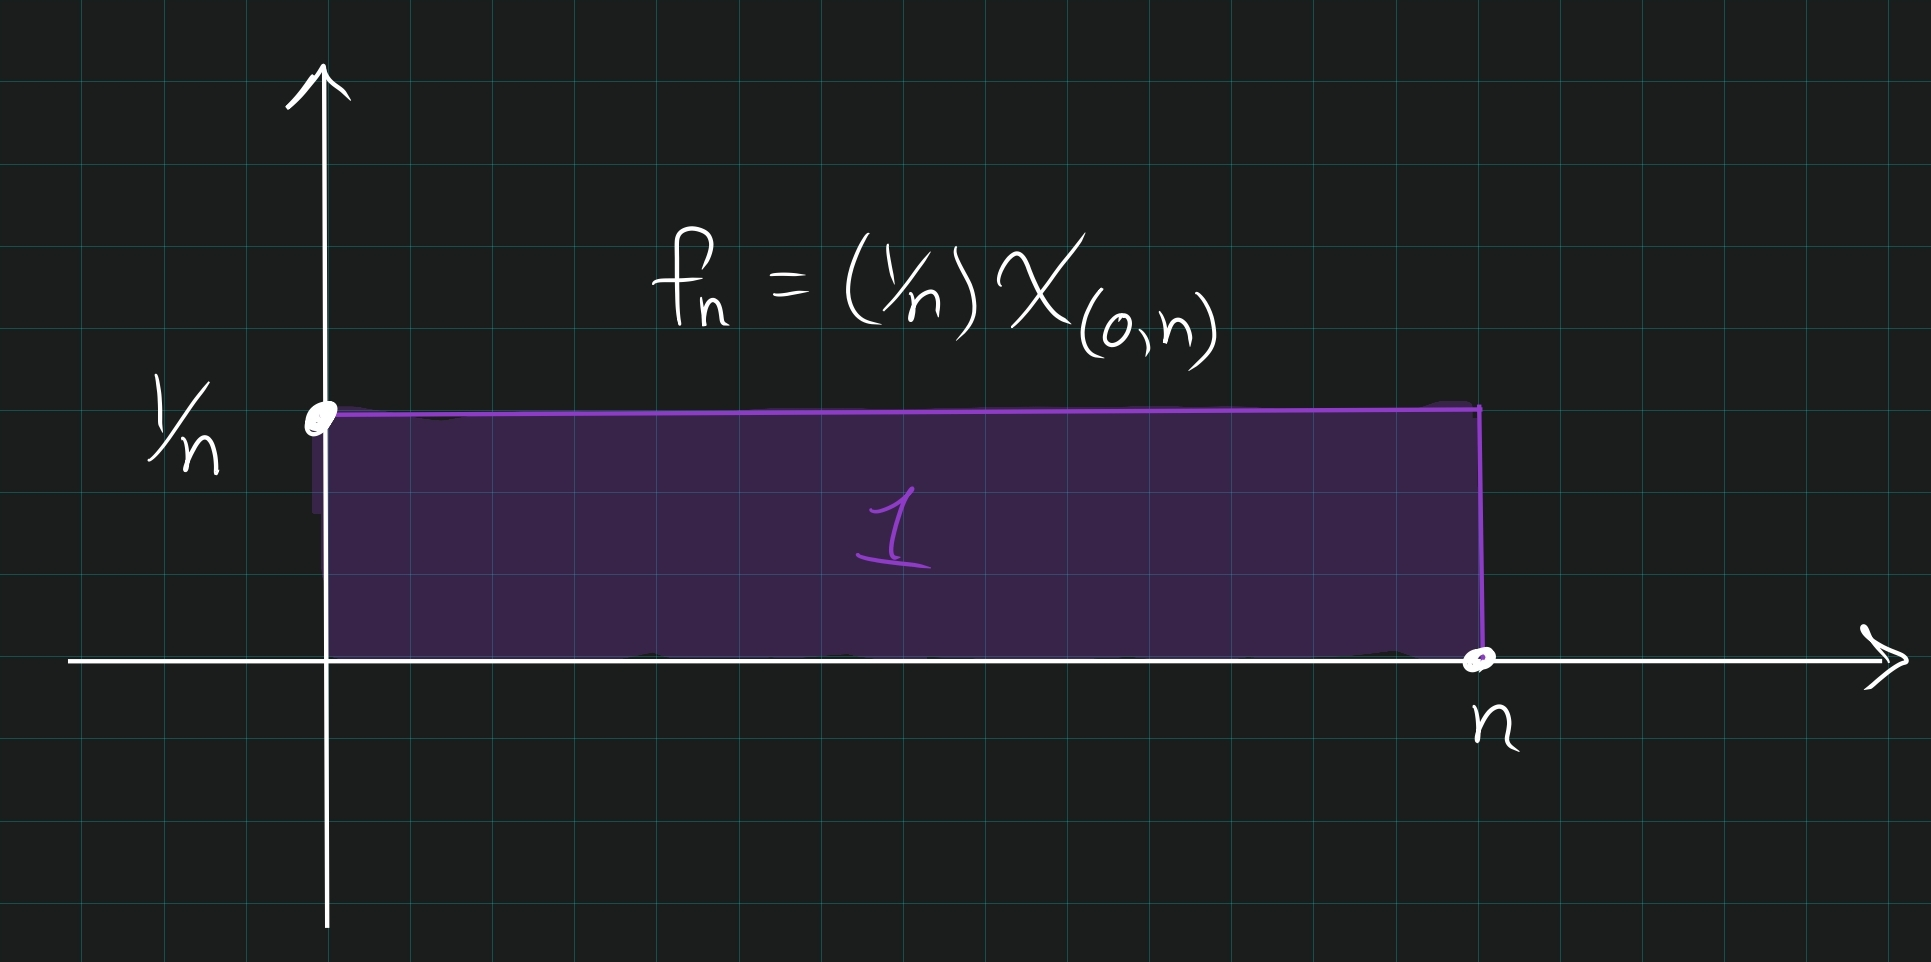
\includegraphics{figures/image_2021-05-21-16-38-30.png}
  \caption{image\_2021-05-21-16-38-30}
  \end{figure}
\item
  \(f_n = \chi_{(n, n+1)}\) (skateboard to infinity). This satisfies 2,3
  but not 1, 4.

  \begin{figure}
  \centering
  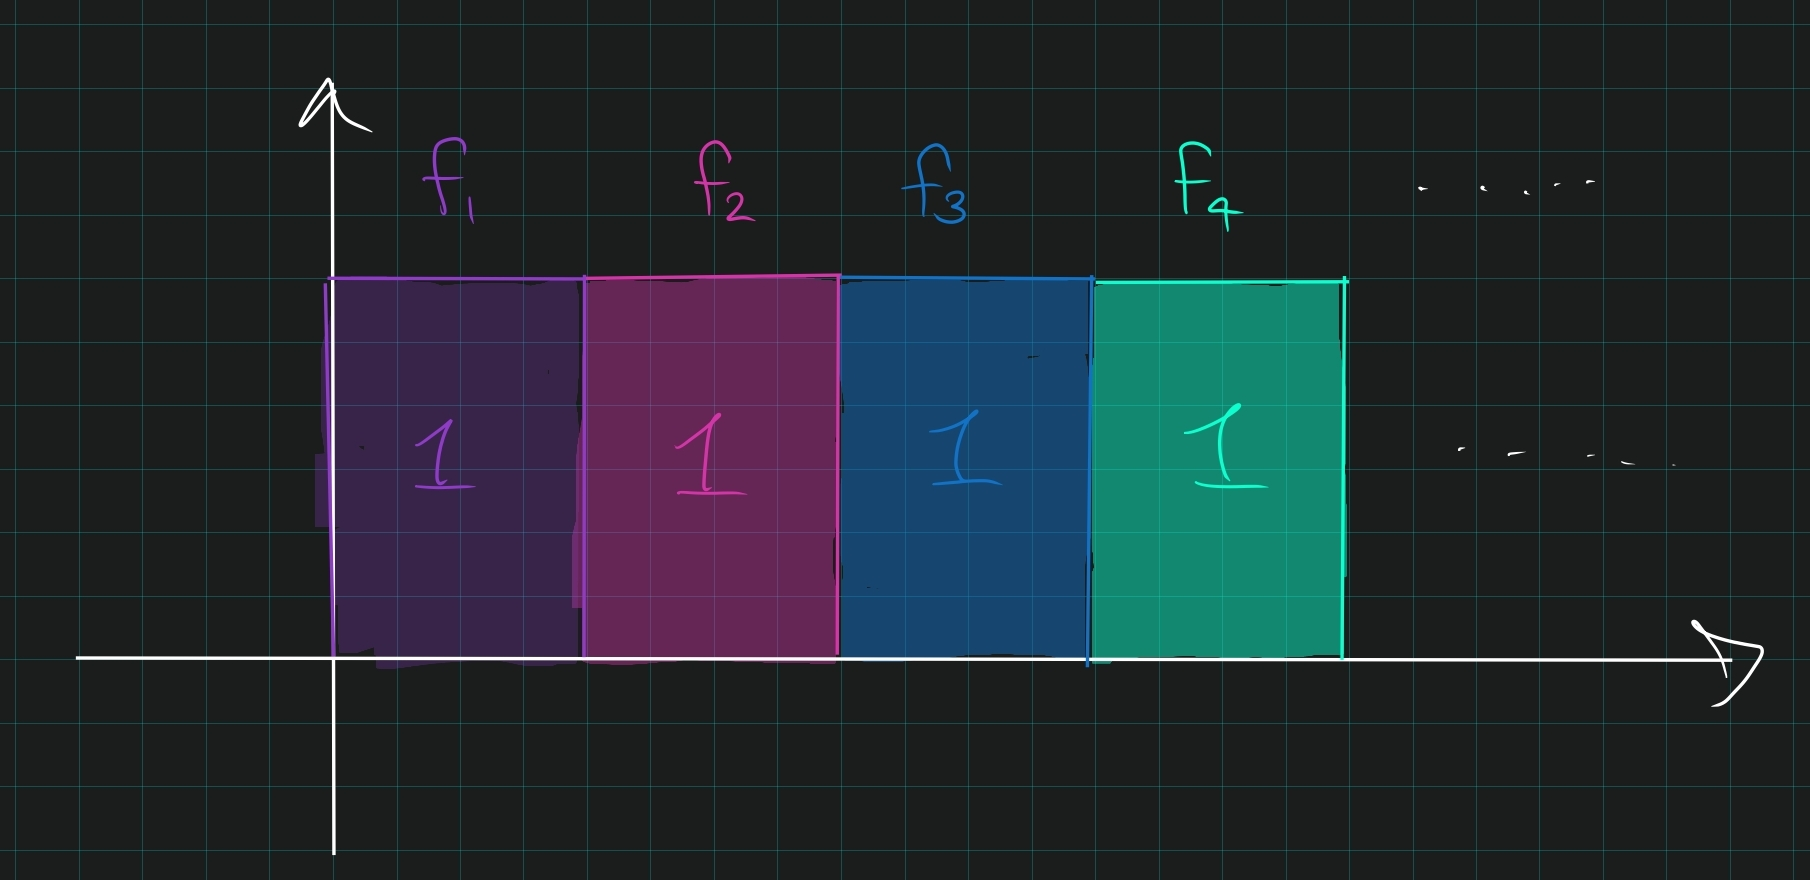
\includegraphics{figures/image_2021-05-21-16-42-08.png}
  \caption{image\_2021-05-21-16-42-08}
  \end{figure}
\item
  \(f_n = n\chi_{(0, \frac 1 n)}\). This satisfies 3 but not 1,2,4.

  \begin{figure}
  \centering
  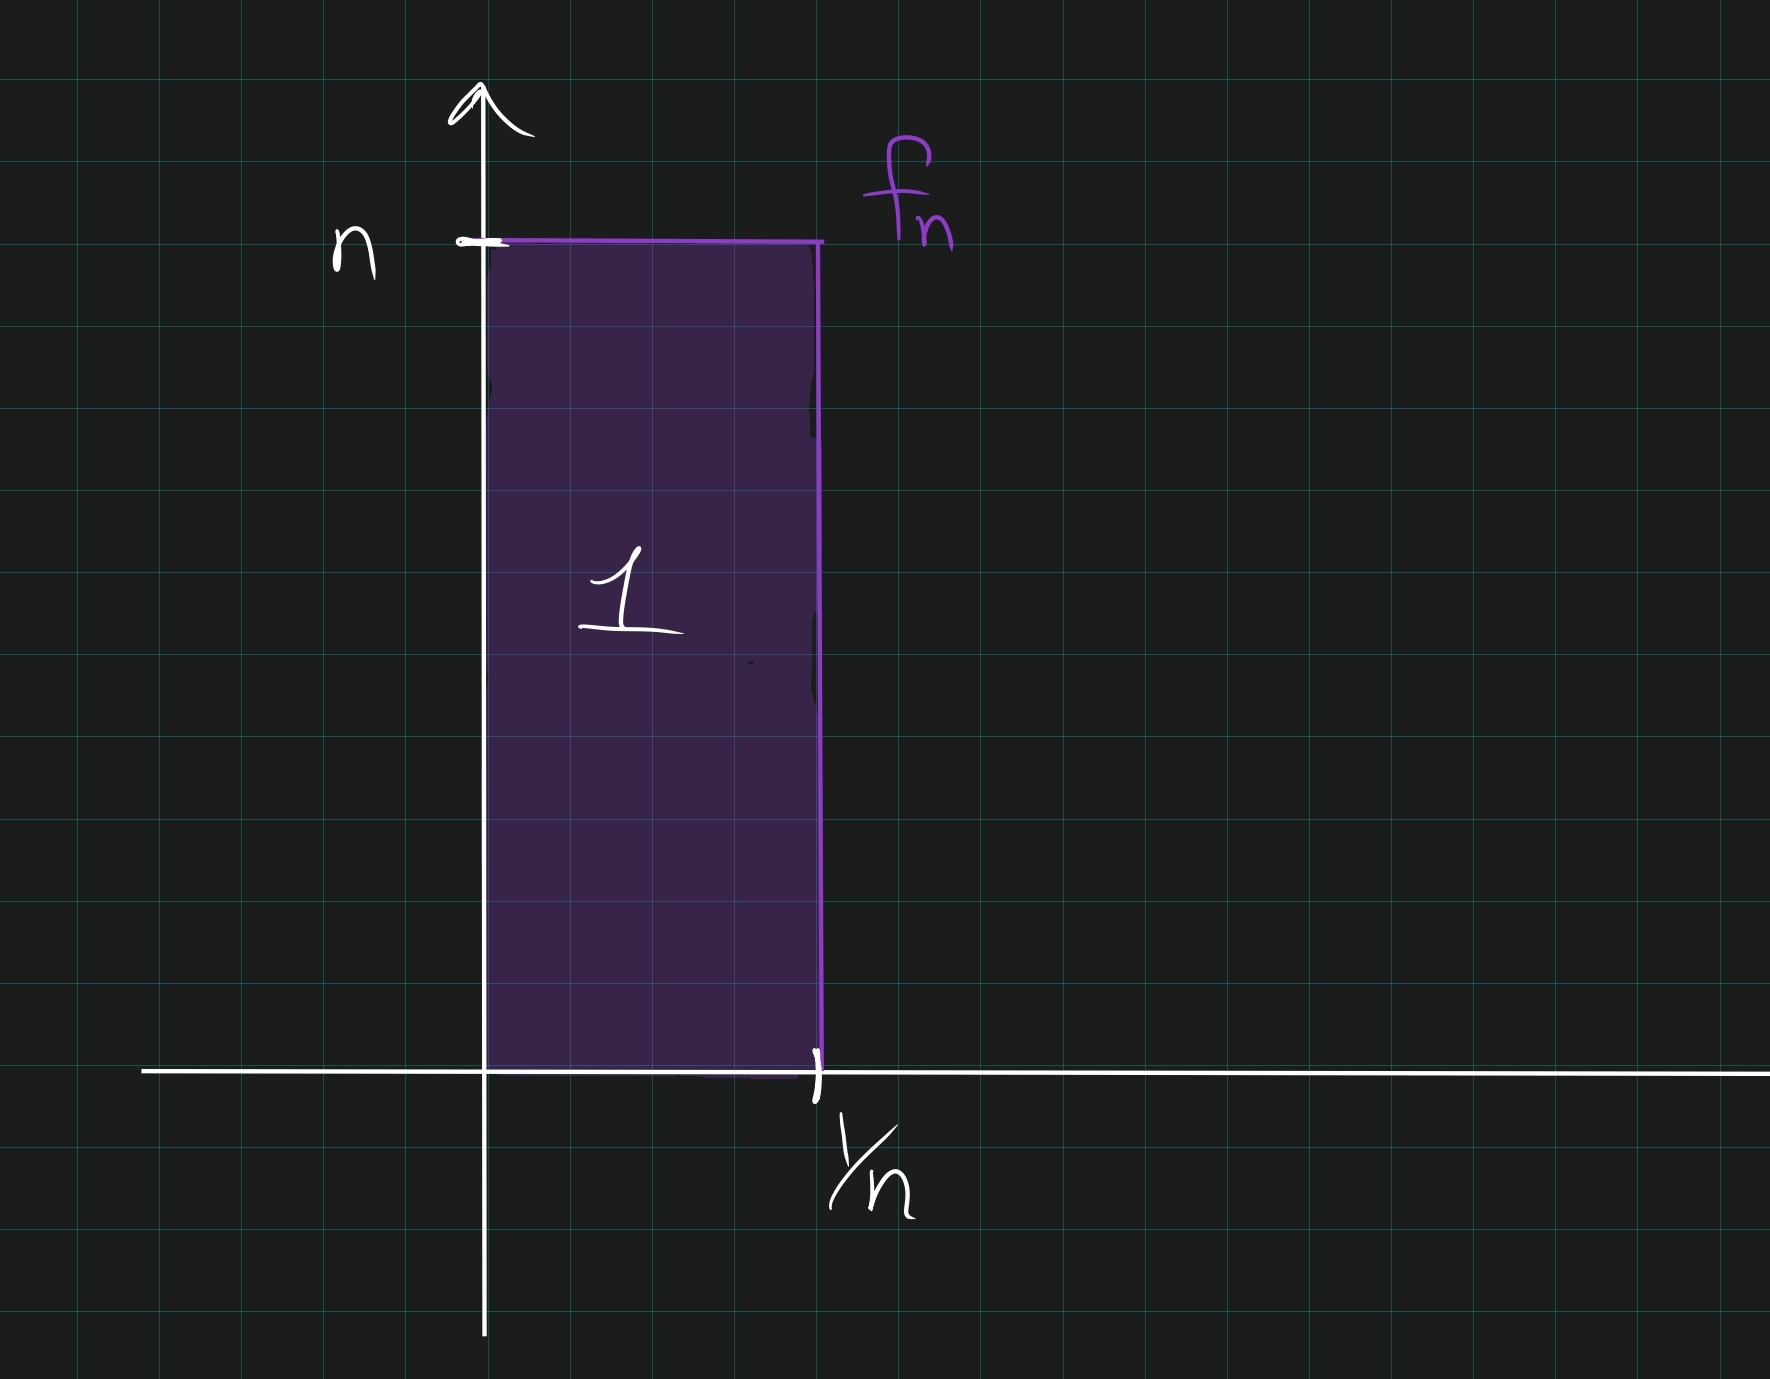
\includegraphics{figures/image_2021-05-21-16-54-38.png}
  \caption{image\_2021-05-21-16-54-38}
  \end{figure}
\item
  \(f_n:\) one can construct a sequence where \(f_n \to 0\) in \(L^1\)
  but is not 1,2, or 3. The construction:

  \begin{itemize}
  \tightlist
  \item
    Break \(I\) into \(2\) intervals, let \(f_1\) be the indicator on
    the first half, \(f_2\) the indicator on the second.
  \item
    Break \(I\) into \(2^2=4\) intervals, like \(f_3\) be the indicator
    on the first quarter, \(f_4\) on the second, etc.
  \item
    Break \(I\) into \(2^k\) intervals and cyclic through \(k\)
    indicator functions.
  \end{itemize}

  \begin{figure}
  \centering
  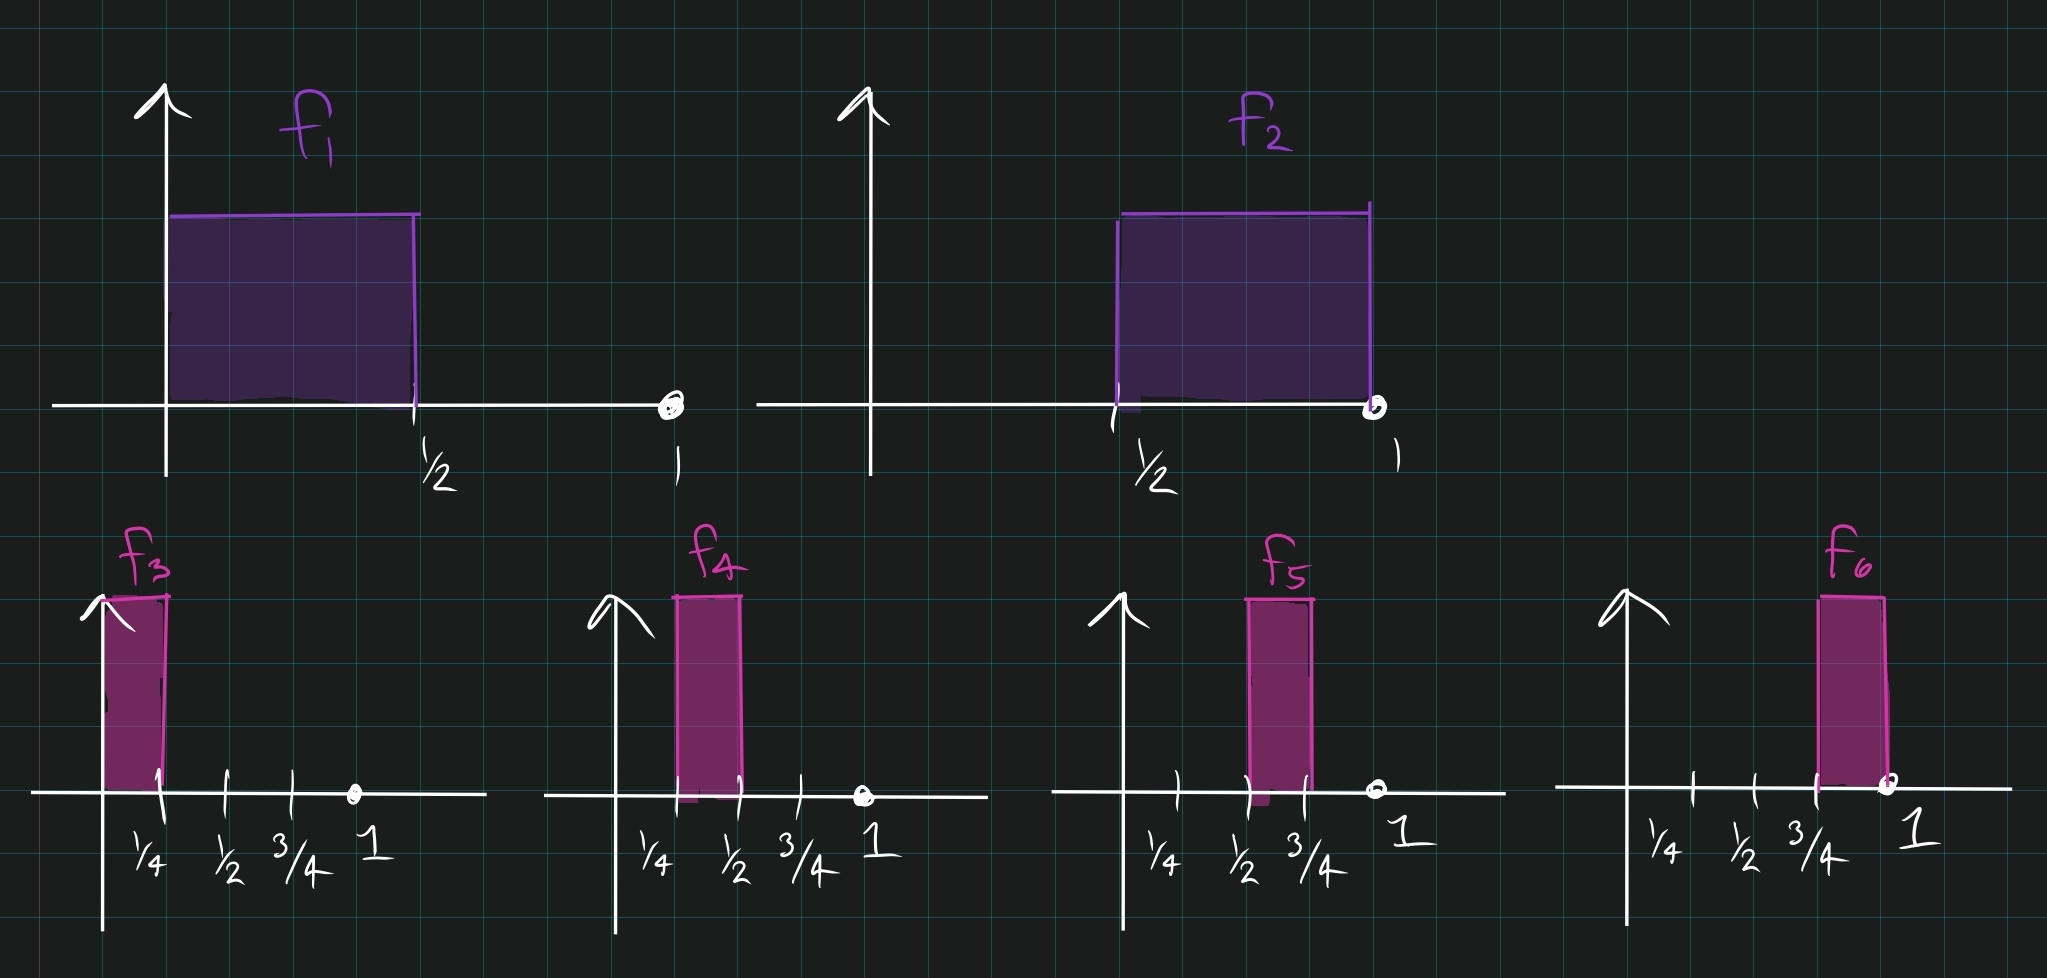
\includegraphics{figures/image_2021-05-21-16-49-09.png}
  \caption{image\_2021-05-21-16-49-09}
  \end{figure}

  \begin{itemize}
  \tightlist
  \item
    Then \(\int f_n = 1/2^n \to 0\), but \(f_n\not\to 0\) pointwise
    since for every \(x\), there are infinitely many \(n\) for which
    \(f_n(x) = 0\) and infinitely many for which \(f_n(x) = 1\).
  \end{itemize}
\end{itemize}

\end{proposition}

\begin{proposition}[Functional analytic properties of $L^1$ and $L^2$]

For any measure space \((X, {\mathcal{M}}, \mu)\),

\begin{itemize}
\tightlist
\item
  \(L^1(X)\) is Banach space.
\item
  \(L^2(X)\) is a (possibly non-separable) Hilbert space.
\end{itemize}

\end{proposition}

\hypertarget{fourier-transform-and-convolution}{%
\section{Fourier Transform and
Convolution}\label{fourier-transform-and-convolution}}

\hypertarget{the-fourier-transform}{%
\subsection{The Fourier Transform}\label{the-fourier-transform}}

\begin{proposition}[?]

If \(\widehat{f} = \widehat{g}\) then \(f=g\) almost everywhere.

\end{proposition}

\begin{proposition}[Riemann-Lebesgue: Fourier transforms have small tails.]

\begin{align*}
f\in L^1 \implies
\widehat{f}(\xi) \rightarrow 0 \text { as }|\xi| \rightarrow \infty
,\end{align*}

if \(f \in L^1\), then \(\widehat{f}\) is continuous and bounded.

\end{proposition}

\begin{proof}[?]

\envlist

\begin{itemize}
\item
  Boundedness:
  \begin{align*}
  {\left\lvert {\widehat{f}(\xi)} \right\rvert} 
  \leq \int {\left\lvert {f} \right\rvert}\cdot {\left\lvert {e^{2\pi i x\cdot \xi }} \right\rvert} 
  = {\left\lVert {f} \right\rVert}_{1}
  .\end{align*}
\item
  Continuity:
\item
  \({\left\lvert {\widehat{f}(\xi_{n}) - \widehat{f} (\xi) } \right\rvert}\)
\item
  Apply DCT to show \(a\overset{n\to\infty}\to 0\).
\end{itemize}

\end{proof}

\begin{theorem}[Fourier Inversion]

\begin{align*}
f(x)=\int_{\mathbb{R}^{n}} \widehat{f}(x) e^{2 \pi i x \cdot \xi} d \xi
.\end{align*}

\end{theorem}

\begin{warnings}

Fubini-Tonelli does not work here!

\end{warnings}

\begin{proof}[?]

Idea: Fubini-Tonelli doesn't work directly, so introduce a convergence
factor, take limits, and use uniqueness of limits.

\begin{itemize}
\tightlist
\item
  Take the modified integral:
\end{itemize}

\begin{align*}
I_{t}(x)
&= \int \widehat{f}(\xi) ~e^{2\pi i x \cdot \xi} ~e^{-\pi t^2 {\left\lvert {\xi} \right\rvert}^2} \\
&= \int \widehat{f}(\xi) \phi(\xi) \\
&= \int f(\xi) \widehat{\phi}(\xi) \\
&= \int f(\xi) \widehat{\widehat{g}}(\xi - x) \\
&= \int f(\xi) g_{t}(x - \xi)  ~d\xi \\
&= \int f(y-x) g_{t}(y) ~dy  \quad (\xi = y-x)\\
&= (f \ast g_{t}) \\
&\to f \text{ in $L^1$ as }t \to 0
.\end{align*}

\begin{itemize}
\item
  We also have
  \begin{align*}
  \lim_{t\to 0} I_{t}(x)
  &= 
  \lim_{t\to 0} \int \widehat{f}(\xi) ~e^{2\pi i x \cdot \xi} ~e^{-\pi t^2 {\left\lvert {\xi} \right\rvert}^2} \\
  &= 
  \lim_{t\to 0} \int \widehat{f}(\xi) \phi(\xi) \\
  &=_{DCT} 
  \int \widehat{f}(\xi) \lim_{t\to 0} \phi(\xi) \\
  &=
  \int \widehat{f}(\xi) ~e^{2\pi i x \cdot \xi} \\
  .\end{align*}
\item
  So
  \begin{align*}
  I_{t}(x) \to \int \widehat{f}(\xi) ~e^{2\pi i x \cdot \xi} ~\text{ pointwise and }~{\left\lVert {I_{t}(x) - f(x)} \right\rVert}_{1} \to 0
  .\end{align*}
\item
  So there is a subsequence \(I_{t_{n}}\) such that
  \(I_{t_{n}}(x) \to f(x)\) almost everywhere
\item
  Thus \(f(x) = \int \widehat{f}(\xi) ~e^{2\pi i x \cdot \xi}\) almost
  everywhere by uniqueness of limits.
\end{itemize}

\end{proof}

\begin{proposition}[Eigenfunction of the Fourier transform]

\begin{align*}
g(x) \coloneqq e^{-\pi {\left\lvert {t} \right\rvert}^2} \implies \widehat{g}(\xi) = g(\xi) {\quad \operatorname{and} \quad}
\widehat{g}_{t}(x) = g(tx) = e^{-\pi t^2 {\left\lvert {x} \right\rvert}^2}
.\end{align*}

\end{proposition}

\hypertarget{approximate-identities}{%
\subsection{Approximate Identities}\label{approximate-identities}}

\begin{example}[of an approximation to the identity.]

\begin{align*}
\phi(x) \coloneqq e^{-\pi x^2}
.\end{align*}

\end{example}

\begin{theorem}[Convolving against an approximate identity converges in $L^1$.]

\begin{align*}
{\left\lVert {f \ast \phi_{t} - f} \right\rVert}_{1} \overset{t\to 0}\to 0
.\end{align*}

\end{theorem}

\begin{proof}[?]

\begin{align*}
{\left\lVert {f - f\ast \phi_{t}} \right\rVert}_1 
&= \int f(x) - \int f(x-y)\phi_{t}(y) ~dy dx \\
&= \int f(x)\int \phi_{t}(y) ~dy - \int f(x-y)\phi_{t}(y) ~dy dx \\
&= \int \int \phi_{t}(y)[f(x) - f(x-y)] ~dy dx \\
&=_{FT} \int \int \phi_{t}(y)[f(x) - f(x-y)] ~dx dy \\
&= \int \phi_{t}(y) \int f(x) - f(x-y) ~dx dy \\
&= \int \phi_{t}(y) {\left\lVert {f - \tau_{y} f} \right\rVert}_1 dy \\
&= \int_{y < \delta} \phi_{t}(y) {\left\lVert {f - \tau_{y} f} \right\rVert}_1 dy  +
\int_{y \geq \delta} \phi_{t}(y) {\left\lVert {f - \tau_{y} f} \right\rVert}_1 dy \\
&\leq \int_{y < \delta} \phi_{t}(y) \varepsilon +
\int_{y \geq \delta} \phi_{t}(y) \left( {\left\lVert {f} \right\rVert}_1 + {\left\lVert {\tau_{y} f} \right\rVert}_1 \right) dy \quad\text{by continuity in } L^1 \\
&\leq \varepsilon + 
2{\left\lVert {f} \right\rVert}_1 \int_{y \geq \delta} \phi_{t}(y) dy \\
&\leq \varepsilon + 2{\left\lVert {f} \right\rVert}_1 \cdot \varepsilon \quad\text{since $\phi_{t}$ has small tails} \\
&\overset{{\varepsilon}\to 0}\to 0 
.\end{align*}

\end{proof}

\begin{theorem}[Convolutions vanish at infinity]

\begin{align*}
f,g \in L^1 \text{ and  bounded}  \implies \lim_{|x| \rightarrow \infty} (f * g)(x) = 0
.\end{align*}

\end{theorem}

\begin{proof}[?]

\begin{itemize}
\item
  Choose \(M \geq f,g\).
\item
  By small tails, choose \(N\) such that
  \(\int_{B_{N}^c} {\left\lvert {f} \right\rvert}, \int_{B_{n}^c} {\left\lvert {g} \right\rvert} < \varepsilon\)
\item
  Note
  \begin{align*}
  {\left\lvert {f \ast g} \right\rvert} \leq \displaystyle\int {\left\lvert {f(x-y)} \right\rvert} ~{\left\lvert {g(y)} \right\rvert} ~dy \coloneqq I
  .\end{align*}
\item
  Use
  \({\left\lvert {x} \right\rvert} \leq {\left\lvert {x-y} \right\rvert} + {\left\lvert {y} \right\rvert}\),
  take \({\left\lvert {x} \right\rvert}\geq 2N\) so either
  \begin{align*}
  {\left\lvert {x-y} \right\rvert} \geq N \implies I \leq \int_{\left\{{x-y \geq N}\right\}} {\left\lvert {f(x-y)} \right\rvert}M ~dy\leq \varepsilon M \to 0
  \end{align*}
  then
  \begin{align*}
  {\left\lvert {y} \right\rvert} \geq N \implies I \leq \int_{\left\{{y \geq N}\right\}} M{\left\lvert {g(y)} \right\rvert} ~dy\leq  M \varepsilon \to 0
  .\end{align*}
\end{itemize}

\end{proof}

\begin{proposition}[Corollary of Young's inequality]

Take \(q = 1\) in Young's inequality to obtain
\begin{align*}
{\left\lVert {f \ast g} \right\rVert}_{p} \leq {\left\lVert {f} \right\rVert}p {\left\lVert {g} \right\rVert}1
.\end{align*}

\end{proposition}

\begin{proposition}[$L^1$ is closed under convolution.]

If \(f, g \in L^1\) then \(f\ast g\in L^1\).

\end{proposition}

\hypertarget{functional-analysis-1}{%
\section{Functional Analysis}\label{functional-analysis-1}}

\hypertarget{theorems-1}{%
\subsection{Theorems}\label{theorems-1}}

\begin{fact}[Pythagoras]

\begin{align*}
{\left\langle {v},~{w} \right\rangle} = 0 \implies {\left\lVert {v+w} \right\rVert} = {\left\lVert {v} \right\rVert} + {\left\lVert {w} \right\rVert}
.\end{align*}

\end{fact}

\begin{theorem}[Bessel's Inequality]

For any orthonormal set
\(\left\{{u_{n}}\right\} \subseteq {\mathcal{H}}\) a Hilbert space (not
necessarily a basis),
\begin{align*}
\left\|x-\sum_{n=1}^{N}\left\langle x, u_{n}\right\rangle u_{n}\right\|^{2}=\|x\|^{2}-\sum_{n=1}^{N}\left|\left\langle x, u_{n}\right\rangle\right|^{2}
\end{align*}
and thus
\begin{align*}
\sum_{n=1}^{\infty}\left|\left\langle x, u_{n}\right\rangle\right|^{2} \leq\|x\|^{2}
.\end{align*}

\end{theorem}

\begin{proof}[of Bessel's inequality]

\envlist

\begin{itemize}
\item
  Let
  \(S_{N} = \sum_{n=1}^N {\left\langle {x},~{u_{n}} \right\rangle} u_{n}\)
  \begin{align*}
  {\left\lVert {x - S_{N}} \right\rVert}^2 
  &= {\left\langle {x - S_{n}},~{x - S_{N}} \right\rangle} \\
  &= {\left\lVert {x} \right\rVert}^2 + {\left\lVert {S_{N}} \right\rVert}^2 - 2\Re{\left\langle {x},~{S_{N}} \right\rangle} \\
  &= {\left\lVert {x} \right\rVert}^2 + {\left\lVert {S_{N}} \right\rVert}^2 - 2\Re {\left\langle {x},~{\sum_{n=1}^N {\left\langle {x},~{u_{n}} \right\rangle}u_{n}} \right\rangle} \\
  &= {\left\lVert {x} \right\rVert}^2 + {\left\lVert {S_{N}} \right\rVert}^2 - 2\Re \sum_{n=1}^N {\left\langle {x},~{ {\left\langle {x},~{u_{n}} \right\rangle}u_{n}} \right\rangle} \\
  &= {\left\lVert {x} \right\rVert}^2 + {\left\lVert {S_{N}} \right\rVert}^2 - 2\Re \sum_{n=1}^N \overline{{\left\langle {x},~{u_{n}} \right\rangle}}{\left\langle {x},~{u_{n}} \right\rangle} \\
  &= {\left\lVert {x} \right\rVert}^2 + \left\|\sum_{n=1}^N {\left\langle {x},~{u_{n}} \right\rangle} u_{n}\right\|^2 - 2 \sum_{n=1}^N {\left\lvert {{\left\langle {x},~{u_{n}} \right\rangle}} \right\rvert}^2 \\
  &= {\left\lVert {x} \right\rVert}^2 + \sum_{n=1}^N {\left\lvert {{\left\langle {x},~{u_{n}} \right\rangle}} \right\rvert}^2 - 2 \sum_{n=1}^N {\left\lvert {{\left\langle {x},~{u_{n}} \right\rangle}} \right\rvert}^2 \\
  &= {\left\lVert {x} \right\rVert}^2 - \sum_{n=1}^N {\left\lvert {{\left\langle {x},~{u_{n}} \right\rangle}} \right\rvert}^2
  .\end{align*}
\item
  By continuity of the norm and inner product, we have
  \begin{align*}
  \lim_{N\to\infty} {\left\lVert {x - S_{N}} \right\rVert}^2 
  &= \lim_{N\to\infty} {\left\lVert {x} \right\rVert}^2 - \sum_{n=1}^N {\left\lvert {{\left\langle {x},~{u_{n}} \right\rangle}} \right\rvert}^2 \\
  \implies {\left\lVert {x - \lim_{N\to\infty} S_{N}} \right\rVert}^2 &= {\left\lVert {x} \right\rVert}^2 - \lim_{N\to\infty}\sum_{n=1}^N {\left\lvert {{\left\langle {x},~{u_{n}} \right\rangle}} \right\rvert}^2\\
  \implies 
  {\left\lVert {x - \sum_{n=1}^\infty {\left\langle {x},~{u_{n}} \right\rangle} u_{n}} \right\rVert}^2 &= {\left\lVert {x} \right\rVert}^2 - 
  \sum_{n=1}^\infty {\left\lvert {{\left\langle {x},~{u_{n}} \right\rangle}} \right\rvert}^2
  .\end{align*}
\item
  Then noting that \(0 \leq {\left\lVert {x - S_{N}} \right\rVert}^2\),
  \begin{align*}
  0 &\leq 
  {\left\lVert {x} \right\rVert}^2 - 
  \sum_{n=1}^\infty {\left\lvert {{\left\langle {x},~{u_{n}} \right\rangle}} \right\rvert}^2 \\
  \implies 
  \sum_{n=1}^\infty {\left\lvert {{\left\langle {x},~{u_{n}} \right\rangle}} \right\rvert}^2 &\leq 
  {\left\lVert {x} \right\rVert}^2 \hfill\blacksquare
  .\end{align*}
\end{itemize}

\end{proof}

\begin{theorem}[Riesz Representation for Hilbert Spaces]

If \(\Lambda\) is a continuous linear functional on a Hilbert space
\(H\), then there exists a unique \(y \in H\) such that
\begin{align*}
\forall x\in H,\quad \Lambda(x) = {\left\langle {x},~{y} \right\rangle}
.\end{align*}

\end{theorem}

\begin{proof}[?]

\envlist

\begin{itemize}
\tightlist
\item
  Define \(M \coloneqq\ker \Lambda\).
\item
  Then \(M\) is a closed subspace and so \(H = M \oplus M^\perp\)
\item
  There is some \(z\in M^\perp\) such that
  \({\left\lVert {z} \right\rVert} = 1\).
\item
  Set \(u \coloneqq\Lambda(x) z - \Lambda(z) x\)
\item
  Check
\end{itemize}

\begin{align*}\Lambda(u) = \Lambda(\Lambda(x) z - \Lambda(z) x) = \Lambda(x) \Lambda(z) - \Lambda(z) \Lambda(x) = 0 \implies u\in M\end{align*}

\begin{itemize}
\tightlist
\item
  Compute
\end{itemize}

\begin{align*}
0 &= {\left\langle {u},~{z} \right\rangle} \\ 
&= {\left\langle {\Lambda(x) z - \Lambda(z) x},~{z} \right\rangle} \\
&= {\left\langle {\Lambda(x) z},~{z} \right\rangle} - {\left\langle {\Lambda(z) x},~{z} \right\rangle} \\
&= \Lambda(x) {\left\langle {z},~{z} \right\rangle} - \Lambda(z) {\left\langle {x},~{z} \right\rangle} \\
&= \Lambda(x) {\left\lVert {z} \right\rVert}^2 - \Lambda(z) {\left\langle {x},~{z} \right\rangle} \\
&= \Lambda(x) - \Lambda(z) {\left\langle {x},~{z} \right\rangle} \\
&= \Lambda(x) -  {\left\langle {x},~{\overline{\Lambda(z)} z} \right\rangle}
,\end{align*}

\begin{itemize}
\tightlist
\item
  Choose \(y \coloneqq\overline{\Lambda(z)} z\).
\item
  Check uniqueness:
\end{itemize}

\begin{align*}
{\left\langle {x},~{y} \right\rangle} &= {\left\langle {x},~{y'} \right\rangle} \quad\forall x \\
\implies  {\left\langle {x},~{y-y'} \right\rangle} &= 0 \quad\forall x \\
\implies {\left\langle {y-y'},~{y-y'} \right\rangle} &= 0 \\
\implies {\left\lVert {y-y'} \right\rVert} &= 0 \\
\implies y-y' &= \mathbf{0} \implies y = y'
.\end{align*}

\end{proof}

\begin{theorem}[Functionals are continuous if and only if bounded]

Let \(L:X \to {\mathbb{C}}\) be a linear functional, then the following
are equivalent:

\begin{enumerate}
\def\labelenumi{\arabic{enumi}.}
\tightlist
\item
  \(L\) is continuous
\item
  \(L\) is continuous at zero
\item
  \(L\) is bounded, i.e.~\(\exists c\geq 0\) such that
  \({\left\lvert {L(x)} \right\rvert} \leq c {\left\lVert {x} \right\rVert}\)
  for all \(x\in H\)
\end{enumerate}

\end{theorem}

\begin{proof}[?]

\(2 \implies 3\): Choose \(\delta < 1\) such that
\begin{align*}
{\left\lVert {x} \right\rVert} \leq \delta \implies {\left\lvert {L(x)} \right\rvert} < 1.
\end{align*}
Then
\begin{align*}
{\left\lvert {L(x)} \right\rvert} 
&= {\left\lvert {L\left( \frac{{\left\lVert {x} \right\rVert}}{\delta} \frac{\delta }{{\left\lVert {x} \right\rVert}} x \right)} \right\rvert} \\
&= \frac{{\left\lVert {x} \right\rVert}}{\delta} ~{\left\lvert {L\left( \delta \frac{x }{{\left\lVert {x} \right\rVert}} \right)} \right\rvert} \\
&\leq \frac{{\left\lVert {x} \right\rVert}}{\delta} 1
,\end{align*}
so we can take \(c = \frac 1 \delta\). \(\hfill\blacksquare\)

\(3 \implies 1\):

We have
\({\left\lvert {L(x-y)} \right\rvert} \leq c{\left\lVert {x-y} \right\rVert}\),
so given \(\varepsilon \geq 0\) simply choose
\(\delta = \frac \varepsilon c\).

\end{proof}

\begin{theorem}[The operator norm is a norm]

If \(H\) is a Hilbert space, then
\((H {}^{ \vee }, {\left\lVert {{-}} \right\rVert}_{\text{op}})\) is a
normed space.

\end{theorem}

\begin{proof}[?]

The only nontrivial property is the triangle inequality, but
\begin{align*}
{\left\lVert {L_{1} + L_{2}} \right\rVert}_{^{\operatorname{op}}} = \sup {\left\lvert {L_{1}(x) + L_{2}(x)} \right\rvert} \leq \sup {\left\lvert {L_{1}(x)} \right\rvert} + {\left\lvert {\sup L_{2}(x)} \right\rvert} = {\left\lVert {L_{1}} \right\rVert}_{^{\operatorname{op}}}+ {\left\lVert {L_{2}} \right\rVert}_{^{\operatorname{op}}}
.\end{align*}

\end{proof}

\begin{theorem}[The operator norm on $X\dual$ yields a Banach space]

If \(X\) is a normed vector space, then
\((X {}^{ \vee }, {\left\lVert {{-}} \right\rVert}_{\text{op}})\) is a
Banach space.

\end{theorem}

\begin{proof}[?]

\envlist

\begin{itemize}
\item
  Let \(\left\{{L_{n}}\right\}\) be Cauchy in \(X {}^{ \vee }\).
\item
  Then for all \(x\in C\),
  \(\left\{{L_{n}(x)}\right\} \subset {\mathbb{C}}\) is Cauchy and
  converges to something denoted \(L(x)\).
\item
  Need to show \(L\) is continuous and
  \({\left\lVert {L_{n} - L} \right\rVert} \to 0\).
\item
  Since \(\left\{{L_{n}}\right\}\) is Cauchy in \(X {}^{ \vee }\),
  choose \(N\) large enough so that
  \begin{align*}
  n, m \geq N \implies {\left\lVert {L_{n} - L_{m}} \right\rVert} < \varepsilon \implies {\left\lvert {L_{m}(x) - L_{n}(x)} \right\rvert} < \varepsilon \quad \forall x {~\mathrel{\Big|}~}{\left\lVert {x} \right\rVert} = 1
  .\end{align*}
\item
  Take \(n\to \infty\) to obtain
  \begin{align*}m \geq N 
  &\implies {\left\lvert {L_{m}(x) - L(x)} \right\rvert} < \varepsilon \quad \forall x {~\mathrel{\Big|}~}{\left\lVert {x} \right\rVert} = 1\\
  &\implies {\left\lVert {L_{m} - L} \right\rVert} < \varepsilon \to 0
  .\end{align*}
\item
  Continuity:
  \begin{align*}
  {\left\lvert {L(x)} \right\rvert} &= {\left\lvert {L(x) - L_{n}(x) + L_{n}(x)} \right\rvert} \\
  &\leq  {\left\lvert {L(x) - L_{n}(x)} \right\rvert} + {\left\lvert {L_{n}(x)} \right\rvert} \\
  &\leq \varepsilon {\left\lVert {x} \right\rVert} + c{\left\lVert {x} \right\rVert} \\
  &= (\varepsilon + c){\left\lVert {x} \right\rVert} \hfill\blacksquare
  .\end{align*}
\end{itemize}

\end{proof}

\begin{theorem}[Riesz-Fischer]

Let \(U = \left\{{u_{n}}\right\}_{n=1}^\infty\) be an orthonormal set
(not necessarily a basis), then

\begin{enumerate}
\def\labelenumi{\arabic{enumi}.}
\tightlist
\item
  There is an isometric surjection
\end{enumerate}

\begin{align*}
\mathcal{H} &\to \ell^2({\mathbb{N}}) \\
\mathbf{x} &\mapsto \left\{{{\left\langle {\mathbf{x}},~{\mathbf{u}_{n}} \right\rangle}}\right\}_{n=1}^\infty
\end{align*}

i.e.~if \(\left\{{a_{n}}\right\} \in \ell^2({\mathbb{N}})\), so
\(\sum {\left\lvert {a_{n}} \right\rvert}^2 < \infty\), then there
exists a \(\mathbf{x} \in \mathcal{H}\) such that
\begin{align*}
a_{n} = {\left\langle {\mathbf{x}},~{\mathbf{u}_{n}} \right\rangle} \quad \forall n.
\end{align*}

\begin{enumerate}
\def\labelenumi{\arabic{enumi}.}
\setcounter{enumi}{1}
\tightlist
\item
  \(\mathbf{x}\) can be chosen such that
  \begin{align*}
  {\left\lVert {\mathbf{x}} \right\rVert}^2 = \sum {\left\lvert {a_{n}} \right\rvert}^2
  \end{align*}
\end{enumerate}

\begin{quote}
Note: the choice of \(\mathbf{x}\) is unique \(\iff\)
\(\left\{{u_{n}}\right\}\) is \textbf{complete},
i.e.~\({\left\langle {\mathbf{x}},~{\mathbf{u}_{n}} \right\rangle} = 0\)
for all \(n\) implies \(\mathbf{x} = \mathbf{0}\).
\end{quote}

\end{theorem}

\begin{proof}[?]

\envlist

\begin{itemize}
\tightlist
\item
  Given \(\left\{{a_{n}}\right\}\), define
  \(S_{N} = \sum^N a_{n} \mathbf{u}_{n}\).
\item
  \(S_{N}\) is Cauchy in \(\mathcal{H}\) and so \(S_{N} \to \mathbf{x}\)
  for some \(\mathbf{x} \in \mathcal{H}\).
\item
  \({\left\langle {x},~{u_{n}} \right\rangle} = {\left\langle {x - S_{N}},~{u_{n}} \right\rangle} + {\left\langle {S_{N}},~{u_{n}} \right\rangle} \to a_{n}\)
\item
  By construction,
  \({\left\lVert {x-S_{N}} \right\rVert}^2 = {\left\lVert {x} \right\rVert}^2 - \sum^N {\left\lvert {a_{n}} \right\rvert}^2 \to 0\),
  so
  \({\left\lVert {x} \right\rVert}^2 = \sum^\infty {\left\lvert {a_{n}} \right\rvert}^2\).
\end{itemize}

\end{proof}

\hypertarget{extra-problems-undergrad-review}{%
\section{Extra Problems: Undergrad
Review}\label{extra-problems-undergrad-review}}

\hypertarget{extra-problems-measure-theory}{%
\section{Extra Problems: Measure
Theory}\label{extra-problems-measure-theory}}

\hypertarget{greatest-hits}{%
\subsection{Greatest Hits}\label{greatest-hits}}

\begin{itemize}
\item
  \(\star\): Show that for \(E\subseteq {\mathbb{R}}^n\), TFAE:

  \begin{enumerate}
  \def\labelenumi{\arabic{enumi}.}
  \tightlist
  \item
    \(E\) is measurable
  \item
    \(E = H\cup Z\) here \(H\) is \(F_\sigma\) and \(Z\) is null
  \item
    \(E = V\setminus Z'\) where \(V\in G_\delta\) and \(Z'\) is null.
  \end{enumerate}
\item
  \(\star\): Show that if \(E\subseteq {\mathbb{R}}^n\) is measurable
  then
  \(m(E) = \sup \left\{{ m(K) {~\mathrel{\Big|}~}K\subset E\text{ compact}}\right\}\)
  iff for all \({\varepsilon}> 0\) there exists a compact
  \(K\subseteq E\) such that \(m(K) \geq m(E) - {\varepsilon}\).
\item
  \(\star\): Show that cylinder functions are measurable, i.e.~if \(f\)
  is measurable on \({\mathbb{R}}^s\), then \(F(x, y) \coloneqq f(x)\)
  is measurable on \({\mathbb{R}}^s\times{\mathbb{R}}^t\) for any \(t\).
\item
  \(\star\): Prove that the Lebesgue integral is translation invariant,
  i.e.~if \(\tau_h(x) = x+h\) then \(\int \tau_h f = \int f\).
\item
  \(\star\): Prove that the Lebesgue integral is dilation invariant,
  i.e.~if \(f_\delta(x) = {f({x\over \delta}) \over \delta^n}\) then
  \(\int f_\delta = \int f\).
\item
  \(\star\): Prove continuity in \(L^1\), i.e.
  \begin{align*}
  f \in L^{1} \Longrightarrow \lim _{h \rightarrow 0} \int|f(x+h)-f(x)|=0
  .\end{align*}
\item
  \(\star\): Show that
  \begin{align*}f,g \in L^1 \implies f\ast g \in L^1 {\quad \operatorname{and} \quad} {\left\lVert {f\ast g} \right\rVert}_1 \leq {\left\lVert {f} \right\rVert}_1 {\left\lVert {g} \right\rVert}_1.\end{align*}
\item
  \(\star\): Show that if \(X\subseteq {\mathbb{R}}\) with
  \(\mu(X) < \infty\) then
  \begin{align*}  
  {\left\lVert {f} \right\rVert}_p \overset{p\to\infty}\to {\left\lVert {f} \right\rVert}_\infty
  .\end{align*}
\end{itemize}

\hypertarget{by-topic}{%
\subsection{By Topic}\label{by-topic}}

\hypertarget{topology}{%
\subsubsection{Topology}\label{topology}}

\begin{itemize}
\tightlist
\item
  Show that every compact set is closed and bounded.
\item
  Show that if a subset of a metric space is complete and totally
  bounded, then it is compact.
\item
  Show that if \(K\) is compact and \(F\) is closed with \(K, F\)
  disjoint then \(\operatorname{dist}(K, F) > 0\).
\end{itemize}

\hypertarget{continuity}{%
\subsubsection{Continuity}\label{continuity}}

\begin{itemize}
\tightlist
\item
  Show that a continuous function on a compact set is uniformly
  continuous.
\end{itemize}

\hypertarget{differentiation}{%
\subsubsection{Differentiation}\label{differentiation}}

\begin{itemize}
\tightlist
\item
  Show that if \(f\in C^1({\mathbb{R}})\) and both
  \(\lim_{x\to \infty} f(x)\) and \(\lim_{x\to \infty} f'(x)\) exist,
  then \(\lim_{x\to\infty} f'(x)\) must be zero.
\end{itemize}

\hypertarget{advanced-limitology}{%
\subsubsection{Advanced Limitology}\label{advanced-limitology}}

\begin{itemize}
\tightlist
\item
  If \(f\) is continuous, is it necessarily the case that \(f'\) is
  continuous?
\item
  If \(f_n \to f\), is it necessarily the case that \(f_n'\) converges
  to \(f'\) (or at all)?
\item
  Is it true that the sum of differentiable functions is differentiable?
\item
  Is it true that the limit of integrals equals the integral of the
  limit?
\item
  Is it true that a limit of continuous functions is continuous?
\item
  Show that a subset of a metric space is closed iff it is complete.
\item
  Show that if \(m(E) < \infty\) and \(f_n\to f\) uniformly, then
  \(\lim \int_E f_n = \int_E f\).
\end{itemize}

Uniform Convergence

\begin{itemize}
\tightlist
\item
  Show that a uniform limit of bounded functions is bounded.
\item
  Show that a uniform limit of continuous function is continuous.

  \begin{itemize}
  \tightlist
  \item
    I.e. if \(f_n\to f\) uniformly with each \(f_n\) continuous then
    \(f\) is continuous.
  \end{itemize}
\item
  Show that

  \begin{itemize}
  \tightlist
  \item
    \(f_n: [a, b]\to {\mathbb{R}}\) are continuously differentiable with
    derivatives \(f_n'\)
  \item
    The sequence of derivatives \(f_n'\) converges uniformly to some
    function \(g\)
  \item
    There exists \emph{at least one} point \(x_0\) such that
    \(\lim_n f_n(x_0)\) exists,
  \item
    Then \(f_n \to f\) uniformly to some differentiable \(f\), and
    \(f' = g\).
  \end{itemize}
\item
  Prove that uniform convergence implies pointwise convergence implies
  a.e. convergence, but none of the implications may be reversed.
\item
  Show that \(\sum {x^n \over n!}\) converges uniformly on any compact
  subset of \({\mathbb{R}}\).
\end{itemize}

Measure Theory

\begin{itemize}
\item
  Show that continuity of measure from above/below holds for outer
  measures.
\item
  Show that a countable union of null sets is null.
\end{itemize}

Measurability

\begin{itemize}
\tightlist
\item
  Show that \(f=0\) a.e. iff \(\int_E f = 0\) for every measurable set
  \(E\).
\end{itemize}

Integrability

\begin{itemize}
\tightlist
\item
  Show that if \(f\) is a measurable function, then \(f=0\) a.e. iff
  \(\int f = 0\).
\item
  Show that a bounded function is Lebesgue integrable iff it is
  measurable.
\item
  Show that simple functions are dense in \(L^1\).
\item
  Show that step functions are dense in \(L^1\).
\item
  Show that smooth compactly supported functions are dense in \(L^1\).
\end{itemize}

Convergence

\begin{itemize}
\tightlist
\item
  Prove Fatou's lemma using the Monotone Convergence Theorem.
\item
  Show that if \(\left\{{f_n}\right\}\) is in \(L^1\) and
  \(\sum \int {\left\lvert {f_n} \right\rvert} < \infty\) then
  \(\sum f_n\) converges to an \(L^1\) function and
  \begin{align*}\int \sum f_n = \sum \int f_n.\end{align*}
\end{itemize}

Convolution

\begin{itemize}
\tightlist
\item
  Show that if \(f, g\) are continuous and compactly supported, then so
  is \(f\ast g\).
\item
  Show that if \(f\in L^1\) and \(g\) is bounded, then \(f\ast g\) is
  bounded and uniformly continuous.
\item
  If \(f, g\) are compactly supported, is it necessarily the case that
  \(f\ast g\) is compactly supported?
\item
  Show that under any of the following assumptions, \(f\ast g\) vanishes
  at infinity:

  \begin{itemize}
  \tightlist
  \item
    \(f, g\in L^1\) are both bounded.
  \item
    \(f, g\in L^1\) with just \(g\) bounded.
  \item
    \(f, g\) smooth and compactly supported (and in fact \(f\ast g\) is
    smooth)
  \item
    \(f\in L^1\) and \(g\) smooth and compactly supported (and in fact
    \(f\ast g\) is smooth)
  \end{itemize}
\item
  Show that if \(f\in L^1\) and \(g'\) exists with
  \({\frac{\partial g}{\partial x_i}\,}\) all bounded, then
  \begin{align*}{\frac{\partial }{\partial x_i}\,}(f\ast g) = f \ast {\frac{\partial g}{\partial x_i}\,}\end{align*}
\end{itemize}

Fourier Analysis

\begin{itemize}
\tightlist
\item
  Show that if \(f\in L^1\) then \(\widehat{f}\) is bounded and
  uniformly continuous.
\item
  Is it the case that \(f\in L^1\) implies \(\widehat{f}\in L^1\)?
\item
  Show that if \(f, \widehat{f} \in L^1\) then \(f\) is bounded,
  uniformly continuous, and vanishes at infinity.

  \begin{itemize}
  \tightlist
  \item
    Show that this is not true for arbitrary \(L^1\) functions.
  \end{itemize}
\item
  Show that if \(f\in L^1\) and \(\widehat{f} = 0\) almost everywhere
  then \(f = 0\) almost everywhere.

  \begin{itemize}
  \tightlist
  \item
    Prove that \(\widehat{f} = \widehat{g}\) implies that \(f=g\) a.e.
  \end{itemize}
\item
  Show that if \(f, g \in L^1\) then
  \begin{align*}\int \widehat{f} g = \int f\widehat{g}.\end{align*}

  \begin{itemize}
  \tightlist
  \item
    Give an example showing that this fails if \(g\) is not bounded.
  \end{itemize}
\item
  Show that if \(f\in C^1\) then \(f\) is equal to its Fourier
  \emph{series}.
\end{itemize}

Approximate Identities

\begin{itemize}
\tightlist
\item
  Show that if \(\phi\) is an approximate identity, then
  \begin{align*}{\left\lVert {f\ast \phi_t - f} \right\rVert}_1 \overset{t\to 0}\to 0.\end{align*}

  \begin{itemize}
  \tightlist
  \item
    Show that if additionally
    \({\left\lvert {\phi(x)} \right\rvert} \leq c(1 + {\left\lvert {x} \right\rvert})^{-n-{\varepsilon}}\)
    for some \(c,{\varepsilon}>0\), then this converges is almost
    everywhere.
  \end{itemize}
\item
  Show that is \(f\) is bounded and uniformly continuous and \(\phi_t\)
  is an approximation to the identity, then \(f\ast \phi_t\) uniformly
  converges to \(f\).
\end{itemize}

\(L^p\) Spaces

\begin{itemize}
\tightlist
\item
  Show that if \(E\subseteq {\mathbb{R}}^n\) is measurable with
  \(\mu(E) < \infty\) and \(f\in L^p(X)\) then
  \begin{align*}{\left\lVert {f} \right\rVert}_{L^p(X)} \overset{p\to\infty}\to {\left\lVert {f} \right\rVert}_\infty.\end{align*}
\item
  Is it true that the converse to the DCT holds? I.e. if
  \(\int f_n \to \int f\), is there a \(g\in L^p\) such that \(f_n < g\)
  a.e. for every \(n\)?
\item
  Prove continuity in \(L^p\): If \(f\) is uniformly continuous then for
  all \(p\),
  \begin{align*}{\left\lVert {\tau_h f - f} \right\rVert}_p \overset{h\to 0}\to 0.\end{align*}
\item
  Prove the following inclusions of \(L^p\) spaces for
  \(m(X) < \infty\):
  \begin{align*}
  L^\infty(X) &\subset L^2(X) \subset L^1(X) \\
  \ell^2({\mathbb{Z}}) &\subset \ell^1({\mathbb{Z}}) \subset \ell^\infty({\mathbb{Z}})
  .\end{align*}
\end{itemize}

\hypertarget{unsorted-1}{%
\subsubsection{Unsorted}\label{unsorted-1}}

\begin{proposition}[Volumes of Rectangles]

If \(\left\{{R_j}\right\} \rightrightarrows R\) is a covering of \(R\)
by rectangles,
\begin{align*}
R = \overset{\circ}{\displaystyle\coprod_{j}} R_j &\implies {\left\lvert {R} \right\rvert} = \sum {\left\lvert {R} \right\rvert}_j \\
R \subseteq \displaystyle\bigcup_j R_j &\implies {\left\lvert {R} \right\rvert} \leq \sum {\left\lvert {R} \right\rvert}_j
.\end{align*}

\end{proposition}

\begin{itemize}
\tightlist
\item
  Show that any disjoint intervals is countable.
\item
  Show that every open \(U \subseteq {\mathbb{R}}\) is a countable union
  of disjoint open intervals.
\item
  Show that every open \(U \subseteq {\mathbb{R}}^n\) is a countable
  union of \emph{almost} disjoint closed cubes.
\item
  Show that that Cantor middle-thirds set is compact, totally
  disconnected, and perfect, with outer measure zero.
\item
  Prove the Borel-Cantelli lemma.
\end{itemize}

\hypertarget{rectangles}{%
\subsection{Rectangles}\label{rectangles}}

\hypertarget{outer-measure-1}{%
\subsection{Outer Measure}\label{outer-measure-1}}

\hypertarget{lebesgue-measurable-sets}{%
\subsection{Lebesgue Measurable Sets}\label{lebesgue-measurable-sets}}

\hypertarget{lebesgue-measurable-functions}{%
\subsection{Lebesgue Measurable
Functions}\label{lebesgue-measurable-functions}}

\hypertarget{extra-problems-integration}{%
\section{Extra Problems: Integration}\label{extra-problems-integration}}

\hypertarget{the-lebesgue-integral}{%
\subsection{The Lebesgue Integral}\label{the-lebesgue-integral}}

\hypertarget{l1-as-a-banach-space}{%
\subsection{\texorpdfstring{\(L^1\) as a Banach
Space}{L\^{}1 as a Banach Space}}\label{l1-as-a-banach-space}}

\hypertarget{fubini-and-tonelli}{%
\subsection{Fubini and Tonelli}\label{fubini-and-tonelli}}

\hypertarget{extra-problems-differentiation-and-misc}{%
\section{Extra Problems: Differentiation and
Misc}\label{extra-problems-differentiation-and-misc}}

\hypertarget{section}{%
\subsection{?}\label{section}}

\hypertarget{midterm-exam-2-december-2014}{%
\section{Midterm Exam 2 (December
2014)}\label{midterm-exam-2-december-2014}}

\hypertarget{section-1}{%
\subsection{1}\label{section-1}}

\begin{quote}
Note: (a) is a repeat.
\end{quote}

\begin{itemize}
\tightlist
\item
  Let \(\Lambda\in L^2(X) {}^{ \vee }\).

  \begin{itemize}
  \tightlist
  \item
    Show that
    \(M\coloneqq\left\{{f\in L^2(X) {~\mathrel{\Big|}~}\Lambda(f) = 0}\right\} \subseteq L^2(X)\)
    is a closed subspace, and \(L^2(X) = M \oplus M\perp\).
  \item
    Prove that there exists a unique \(g\in L^2(X)\) such that
    \(\Lambda(f) = \int_X g \mkern 1.5mu\overline{\mkern-1.5muf\mkern-1.5mu}\mkern 1.5mu\).
  \end{itemize}
\end{itemize}

\hypertarget{section-2}{%
\subsection{2}\label{section-2}}

\begin{enumerate}
\def\labelenumi{\alph{enumi}.}
\tightlist
\item
  In parts:
\end{enumerate}

\begin{itemize}
\tightlist
\item
  Given a definition of \(L^\infty({\mathbb{R}}^n)\).
\item
  Verify that \({\left\lVert {{-}} \right\rVert}_\infty\) defines a norm
  on \(L^\infty({\mathbb{R}}^n)\).
\item
  Carefully proved that
  \((L^\infty({\mathbb{R}}^n), {\left\lVert {{-}} \right\rVert}_\infty)\)
  is a Banach space.
\end{itemize}

\begin{enumerate}
\def\labelenumi{\alph{enumi}.}
\setcounter{enumi}{1}
\tightlist
\item
  Prove that for any measurable \(f:{\mathbb{R}}^n \to {\mathbb{C}}\),
  \begin{align*}
  L^1({\mathbb{R}}^n) \cap L^\infty({\mathbb{R}}^n) \subset L^2({\mathbb{R}}^n) {\quad \operatorname{and} \quad} {\left\lVert {f} \right\rVert}_2 \leq {\left\lVert {f} \right\rVert}_1^{1\over 2} \cdot {\left\lVert {f} \right\rVert}_\infty^{1\over 2}
  .\end{align*}
\end{enumerate}

\hypertarget{section-3}{%
\subsection{3}\label{section-3}}

\begin{enumerate}
\def\labelenumi{\alph{enumi}.}
\item
  Prove that if \(f, g: {\mathbb{R}}^n\to {\mathbb{C}}\) is both
  measurable then \(F(x, y) \coloneqq f(x)\) and
  \(h(x, y)\coloneqq f(x-y) g(y)\) is measurable on
  \({\mathbb{R}}^n\times{\mathbb{R}}^n\).
\item
  Show that if
  \(f\in L^1({\mathbb{R}}^n) \cap L^\infty({\mathbb{R}}^n)\) and
  \(g\in L^1({\mathbb{R}}^n)\), then
  \(f\ast g \in L^1({\mathbb{R}}^n) \cap L^\infty({\mathbb{R}}^n)\) is
  well defined, and carefully show that it satisfies the following
  properties:
  \begin{align*}
  {\left\lVert {f\ast g} \right\rVert}_\infty &\leq {\left\lVert {g} \right\rVert}_1 {\left\lVert {f} \right\rVert}_\infty
  {\left\lVert {f\ast g} \right\rVert}_1      &\leq {\left\lVert {g} \right\rVert}_1 {\left\lVert {f} \right\rVert}_1
  {\left\lVert {f\ast g} \right\rVert}_2      &\leq {\left\lVert {g} \right\rVert}_1 {\left\lVert {f} \right\rVert}_2
  .\end{align*}
\end{enumerate}

\begin{quote}
Hint: first show
\({\left\lvert {f\ast g} \right\rvert}^2 \leq {\left\lVert {g} \right\rVert}_1 \qty{ {\left\lvert {f} \right\rvert}^2 \ast {\left\lvert {g} \right\rvert}}\).
\end{quote}

\hypertarget{weierstrass-approximation-theorem}{%
\subsection{4 (Weierstrass Approximation
Theorem)}\label{weierstrass-approximation-theorem}}

\begin{quote}
Note: (a) is a repeat.
\end{quote}

Let \(f: [0, 1]\to {\mathbb{R}}\) be continuous, and prove the
Weierstrass approximation theorem: for any \({\varepsilon}> 0\) there
exists a polynomial \(P\) such that
\({\left\lVert {f - P} \right\rVert}_{\infty} < {\varepsilon}\).

\hypertarget{midterm-exam-1-october-2018}{%
\section{Midterm Exam 1 (October
2018)}\label{midterm-exam-1-october-2018}}

\hypertarget{problem-1}{%
\subsection{Problem 1}\label{problem-1}}

\label{equivalence_of_approximating_measures} Let
\(E \subseteq {\mathbb{R}}^n\) be bounded. Prove the following are
equivalent:

\begin{enumerate}
\def\labelenumi{\arabic{enumi}.}
\item
  For any \(\epsilon>0\) there exists and open set \(G\) and a closed
  set \(F\) such that
  \begin{align*}
  F \subseteq E \subseteq G && m(G\setminus F) < \epsilon
  .\end{align*}
\item
  There exists a \(G_ \delta\) set \(V\) and an \(F_ \sigma\) set \(H\)
  such that
  \begin{align*}
  m(V\setminus H) = 0
  .\end{align*}
\end{enumerate}

\hypertarget{problem-2}{%
\subsection{Problem 2}\label{problem-2}}

Let \(\left\{{ f_k }\right\} _{k=1}^{\infty }\) be a sequence of
extended real-valued Lebesgue measurable functions.

\begin{enumerate}
\def\labelenumi{\alph{enumi}.}
\item
  Prove that \(\sup_k f_k\) is a Lebesgue measurable function.
\item
  Prove that if \(\lim_{k \to \infty } f_k(x)\) exists for every
  \(x \in {\mathbb{R}}^n\) then \(\lim_{k\to \infty } f_k\) is also a
  measurable function.
\end{enumerate}

\hypertarget{problem-3}{%
\subsection{Problem 3}\label{problem-3}}

\hypertarget{a}{%
\subsubsection{a}\label{a}}

Prove that if \(E \subseteq {\mathbb{R}}^n\) is a Lebesgue measurable
set, then for any \(h \in {\mathbb{R}}\) the set
\begin{align*}
E+h \coloneqq\left\{{x + h {~\mathrel{\Big|}~}x\in E }\right\}
\end{align*}
is also Lebesgue measurable and satisfies \(m(E + h) = m(E)\).

\hypertarget{b}{%
\subsubsection{b}\label{b}}

Prove that if \(f\) is a non-negative measurable function on
\({\mathbb{R}}^n\) and \(h\in {\mathbb{R}}^n\) then the function
\begin{align*}
\tau_h d(x) \coloneqq f(x-h)
\end{align*}
is a non-negative measurable function and
\begin{align*}
\int f(x) \,dx= \int f(x-h) \,dx
.\end{align*}

\hypertarget{problem-4}{%
\subsection{Problem 4}\label{problem-4}}

Let \(f: {\mathbb{R}}^n\to {\mathbb{R}}\) be a Lebesgue measurable
function.

\begin{enumerate}
\def\labelenumi{\alph{enumi}.}
\item
  Prove that for all \(\alpha> 0\) ,
  \begin{align*}
  A_ \alpha  \coloneqq\left\{{x\in {\mathbb{R}}^n {~\mathrel{\Big|}~}{\left\lvert { f(x) } \right\rvert} > \alpha}\right\} \implies m(A_ \alpha) \leq {1\over \alpha} \int {\left\lvert {f (x)} \right\rvert} \,dx
  .\end{align*}
\item
  Prove that
  \begin{align*}
  \int {\left\lvert { f(x) } \right\rvert} \,dx= 0 \iff f = 0 \text{ almost everywhere}
  .\end{align*}
\end{enumerate}

\hypertarget{problem-5}{%
\subsection{Problem 5}\label{problem-5}}

Let \(\left\{{ f_k }\right\}_{k=1}^{\infty } \subseteq L^2([0, 1])\) be
a sequence which \emph{converges in \(L^1\)} to a function \(f\).

\begin{enumerate}
\def\labelenumi{\alph{enumi}.}
\item
  Prove that \(f\in L^1([0, 1])\).
\item
  Give an example illustrating that \(f_k\) may not converge to \(f\)
  almost everywhere.
\item
  Prove that \(\left\{{f_k}\right\}\) must contain a subsequence that
  converges to \(f\) almost everywhere.
\end{enumerate}

\hypertarget{midterm-exam-2-november-2018}{%
\section{Midterm Exam 2 (November
2018)}\label{midterm-exam-2-november-2018}}

\hypertarget{problem-1-1}{%
\subsection{Problem 1}\label{problem-1-1}}

Let \(f, g\in L^1([0, 1])\), define \(F(x) = \int_0^x f(y)\,dy\) and
\(G(x) = \int_0^x g(y)\,dy\), and show
\begin{align*}
\int_0^1 F(x)g(x) \,dx = F(1)G(1) - \int_0^1 f(x) G(x) \, dx
.\end{align*}

\hypertarget{problem-2-1}{%
\subsection{Problem 2}\label{problem-2-1}}

Let \(\phi\in L^1({\mathbb{R}}^n)\) such that \(\int \phi = 1\) and
define \(\phi_t(x) = t^{-n}\phi(t^{-1}x)\). Show that if \(f\) is
bounded and uniformly continuous then
\(f\ast \phi_t \overset{t\to 0}\to f\) uniformly.

\hypertarget{problem-3-1}{%
\subsection{Problem 3}\label{problem-3-1}}

Let \(g\in L^\infty([0, 1])\).

\begin{enumerate}
\def\labelenumi{\alph{enumi}.}
\item
  Prove
  \begin{align*}
  {\left\lVert {g} \right\rVert}_{L^p([0, 1])}  \overset{p\to\infty}\to {\left\lVert {g} \right\rVert}_{L^\infty([0, 1])}
  .\end{align*}
\item
  Prove that the map
  \begin{align*}
  \Lambda_g: L^1([0, 1]) &\to {\mathbb{C}}\\
  f &\mapsto \int_0^1 fg
  \end{align*}
  defines an element of \(L^1([0, 1]) {}^{ \vee }\) with
  \({\left\lVert {\Lambda_g} \right\rVert}_{L^1([0, 1]) {}^{ \vee }}= {\left\lVert {g} \right\rVert}_{L^\infty([0, 1])}\).
\end{enumerate}

\hypertarget{problem-4-1}{%
\subsection{Problem 4}\label{problem-4-1}}

See \cref{hilbert_space_exam_question}

\hypertarget{practice-exam-november-2014}{%
\section{Practice Exam (November
2014)}\label{practice-exam-november-2014}}

\hypertarget{problem-1-2}{%
\subsection{Problem 1}\label{problem-1-2}}

Let \(m_*(E)\) denote the Lebesgue outer measure of a set
\(E \subseteq {\mathbb{R}}^n\).

\begin{enumerate}
\def\labelenumi{\alph{enumi}.}
\item
  Prove using the definition of Lebesgue outer measure that
  \begin{align*}
  m \qty{ \displaystyle\bigcup_{j=1}^{\infty } E_j  } \leq \sum_{j=1}^{\infty } m_*(E_j) 
  .\end{align*}
\item
  Prove that for any \(E \subseteq {\mathbb{R}}^n\) and any
  \(\epsilon> 0\) there exists an open set \(G\) with \(E \subseteq G\)
  and
  \begin{align*}
  m_*(E) \leq m_*(G) \leq m_*(E) + \epsilon
  .\end{align*}
\end{enumerate}

\hypertarget{problem-2-2}{%
\subsection{Problem 2}\label{problem-2-2}}

\begin{enumerate}
\def\labelenumi{\alph{enumi}.}
\item
  See \cref{equivalence_of_approximating_measures}
\item
  Let \(f_k\) be a sequence of extended real-valued Lebesgue measurable
  function.

  \begin{enumerate}
  \def\labelenumii{\roman{enumii}.}
  \item
    Prove that \(\inf_k f_k, \sup_k f_k\) are both Lebesgue measurable
    function.

    \emph{Hint: argue that}
    \begin{align*}
    \left\{{x {~\mathrel{\Big|}~}\inf_k f_k(x) < a}\right\} = \displaystyle\bigcup_k \left\{{x {~\mathrel{\Big|}~}f_k(x) < a}\right\}
    .\end{align*}
  \item
    Carefully state Fatou's Lemma and deduce the Monotone Converge
    Theorem from it.
  \end{enumerate}
\end{enumerate}

\hypertarget{problem-3-2}{%
\subsection{Problem 3}\label{problem-3-2}}

\begin{enumerate}
\def\labelenumi{\alph{enumi}.}
\item
  Prove that if \(f, g\in L^+({\mathbb{R}})\) then
  \begin{align*}
  \int(f +g) = \int f + \int g
  .\end{align*}
  Extend this to establish that if
  \(\left\{{ f_k}\right\} \subseteq L^+({\mathbb{R}}^n)\) then
  \begin{align*}
    \int \sum_k f_k = \sum_k \int f_k
    .\end{align*}
\item
  Let
  \(\left\{{E_j}\right\}_{j\in {\mathbb{N}}} \subseteq \mathcal{M}({\mathbb{R}}^n)\)
  with \(E_j \nearrow E\). Use the countable additivity of \(\mu_f\) on
  \(\mathcal{M}({\mathbb{R}}^n)\) established above to show that
  \begin{align*}
    \mu_f(E) = \lim_{j\to \infty } \mu_f(E_j)
    .\end{align*}
\end{enumerate}

\hypertarget{problem-4-2}{%
\subsection{Problem 4}\label{problem-4-2}}

\begin{enumerate}
\def\labelenumi{\alph{enumi}.}
\item
  Show that
  \(f\in L^1({\mathbb{R}}^n) \implies {\left\lvert {f(x)} \right\rvert} < \infty\)
  almost everywhere.
\item
  Show that if \(\left\{{f_k}\right\} \subseteq L^1({\mathbb{R}}^n)\)
  with \(\sum {\left\lVert {f_k} \right\rVert}_1 < \infty\) then
  \(\sum f_k\) converges almost everywhere and in \(L^1\).
\item
  Use the Dominated Convergence Theorem to evaluate
  \begin{align*}
  \lim_{t\to 0} \int_0^1 {e^{tx^2} - 1 \over t} \,dx
  .\end{align*}
\end{enumerate}

\hypertarget{practice-exam-november-2014-1}{%
\section{Practice Exam (November
2014)}\label{practice-exam-november-2014-1}}

\hypertarget{fubini-tonelli}{%
\subsection{1: Fubini-Tonelli}\label{fubini-tonelli}}

\begin{enumerate}
\def\labelenumi{\alph{enumi}.}
\item
  Carefully state Tonelli's theorem for a nonnegative function
  \(F(x, t)\) on \({\mathbb{R}}^n\times{\mathbb{R}}\).
\item
  Let \(f:{\mathbb{R}}^n\to [0, \infty]\) and define
  \begin{align*}
  {\mathcal{A}}\coloneqq\left\{{(x, t) \in {\mathbb{R}}^n\times{\mathbb{R}}{~\mathrel{\Big|}~}0\leq t \leq f(x)}\right\}
  .\end{align*}

  Prove the validity of the following two statements:

  \begin{enumerate}
  \def\labelenumii{\arabic{enumii}.}
  \tightlist
  \item
    \(f\) is Lebesgue measurable on
    \({\mathbb{R}}^{n} \iff {\mathcal{A}}\) is a Lebesgue measurable
    subset of \({\mathbb{R}}^{n+1}\).
  \item
    If \(f\) is Lebesgue measurable on \({\mathbb{R}}^n\) then
    \begin{align*}
    m(\mathcal{A})=\int_{\mathbb{R}^{n}} f(x) d x=\int_{0}^{\infty} m\left(\left\{x \in \mathbb{R}^{n}{~\mathrel{\Big|}~}f(x) \geq t\right\}\right) d t
    .\end{align*}
  \end{enumerate}
\end{enumerate}

\hypertarget{convolutions-and-the-fourier-transform}{%
\subsection{2: Convolutions and the Fourier
Transform}\label{convolutions-and-the-fourier-transform}}

\begin{enumerate}
\def\labelenumi{\alph{enumi}.}
\item
  Let \(f, g\in L^1({\mathbb{R}}^n)\) and give a definition of
  \(f\ast g\).
\item
  Prove that if \(f, g\) are integrable and bounded, then
  \begin{align*}
  (f\ast g)(x) \overset{{\left\lvert {x} \right\rvert}\to\infty}\to 0
  .\end{align*}
\item
  In parts:

  \begin{enumerate}
  \def\labelenumii{\arabic{enumii}.}
  \tightlist
  \item
    Define the \emph{Fourier transform} of an integrable function \(f\)
    on \({\mathbb{R}}^n\).
  \item
    Give an outline of the proof of the Fourier inversion formula.
  \item
    Give an example of a function \(f\in L^1({\mathbb{R}}^n)\) such that
    \(\widehat{f}\) is not in \(L^1({\mathbb{R}}^n)\).
  \end{enumerate}
\end{enumerate}

\hypertarget{hilbert-spaces}{%
\subsection{3: Hilbert Spaces}\label{hilbert-spaces}}

\label{hilbert_space_exam_question}

Let \(\left\{{u_n}\right\}_{n=1}^\infty\) be an orthonormal sequence in
a Hilbert space \(H\).

\begin{enumerate}
\def\labelenumi{\alph{enumi}.}
\item
  Let \(x\in H\) and verify that
  \begin{align*}
  \left\|x-\sum_{n=1}^{N}\left\langle x, u_{n}\right\rangle u_{n}\right\|_H^{2}
  =
  \|x\|_H^{2}-\sum_{n=1}^{N}\left|\left\langle x, u_{n}\right\rangle\right|^{2}
  .\end{align*}
  for any \(N\in {\mathbb{N}}\) and deduce that
  \begin{align*}
  \sum_{n=1}^{\infty}\left|\left\langle x, u_{n}\right\rangle\right|^{2} \leq\|x\|_H^{2}
  .\end{align*}
\item
  Let
  \(\left\{{a_n}\right\}_{n\in {\mathbb{N}}} \in \ell^2({\mathbb{N}})\)
  and prove that there exists an \(x\in H\) such that
  \(a_n = {\left\langle {x},~{u_n} \right\rangle}\) for all
  \(n\in {\mathbb{N}}\), and moreover \(x\) may be chosen such that
  \begin{align*}
  {\left\lVert {x} \right\rVert}_H = \qty{ \sum_{n\in {\mathbb{N}}} {\left\lvert {a_n} \right\rvert}^2}^{1\over 2}
  .\end{align*}
\item
  Prove that if \(\left\{{u_n}\right\}\) is \emph{complete}, Bessel's
  inequality becomes an equality.
\end{enumerate}

\begin{solution}[part b]

\envlist

\begin{itemize}
\item
  Take \(\left\{{a_n}\right\} \in \ell^2\), then note that
  \(\sum {\left\lvert {a_n} \right\rvert}^2 < \infty \implies\) the
  tails vanish.
\item
  Define \(x \coloneqq\displaystyle\lim_{N\to\infty} S_N\) where
  \(S_N = \sum_{k=1}^N a_k u_k\)
\item
  \(\left\{{S_N}\right\}\) is Cauchy and \(H\) is complete, so
  \(x\in H\).
\item
  By construction,
  \begin{align*}
  {\left\langle {x},~{u_n} \right\rangle} = {\left\langle {\sum_k a_k u_k},~{u_n} \right\rangle} = \sum_k a_k {\left\langle {u_k},~{u_n} \right\rangle} = a_n 
  \end{align*}
  since the \(u_k\) are all orthogonal.
\item
  By Pythagoras since the \(u_k\) are normal,
  \begin{align*}
  {\left\lVert {x} \right\rVert}^2 = {\left\lVert {\sum_k a_k u_k} \right\rVert}^2 = \sum_k {\left\lVert {a_k u_k} \right\rVert}^2 = \sum_k {\left\lvert {a_k} \right\rvert}^2
  .\end{align*}
\end{itemize}

\end{solution}

\begin{solution}[part c]

Let \(x\) and \(u_n\) be arbitrary.

\begin{align*}
{\left\langle {x - \sum_{k=1}^\infty {\left\langle {x},~{u_k} \right\rangle}u_k },~{u_n} \right\rangle}
&=
{\left\langle {x},~{u_n} \right\rangle}
-
{\left\langle {\sum_{k=1}^\infty {\left\langle {x},~{u_k} \right\rangle}u_k },~{u_n} \right\rangle} \\
&=
{\left\langle {x},~{u_n} \right\rangle}
-
\sum_{k=1}^\infty  {\left\langle {{\left\langle {x},~{u_k} \right\rangle}u_k },~{u_n} \right\rangle} \\
&=
{\left\langle {x},~{u_n} \right\rangle}
-
\sum_{k=1}^\infty  {\left\langle {x},~{u_k} \right\rangle} {\left\langle {u_k },~{u_n} \right\rangle} \\
&= {\left\langle {x},~{u_n} \right\rangle} - {\left\langle {x},~{u_n} \right\rangle} = 0 \\
\implies 
x - \sum_{k=1}^\infty {\left\langle {x},~{u_k} \right\rangle}u_k &= 0 \quad\text{by completeness}
.\end{align*}

So
\begin{align*}
x = \sum_{k=1}^\infty {\left\langle {x},~{u_k} \right\rangle} u_k
\implies
{\left\lVert {x} \right\rVert}^2 = \sum_{k=1}^\infty {\left\lvert {{\left\langle {x},~{u_k} \right\rangle}} \right\rvert}^2. \hfill\blacksquare
.\end{align*}

\end{solution}

\hypertarget{lp-spaces}{%
\subsection{\texorpdfstring{4: \(L^p\)
Spaces}{4: L\^{}p Spaces}}\label{lp-spaces}}

\begin{enumerate}
\def\labelenumi{\alph{enumi}.}
\item
  Prove Holder's inequality: let \(f\in L^p, g\in L^q\) with \(p, q\)
  conjugate, and show that
  \begin{align*}
  {\left\lVert {fg} \right\rVert}_{p} \leq {\left\lVert {f} \right\rVert}_{p} \cdot {\left\lVert {g} \right\rVert}_{q}
  .\end{align*}
\item
  Prove Minkowski's Inequality:
  \begin{align*}
  1\leq p < \infty \implies {\left\lVert {f+g} \right\rVert}_{p} \leq {\left\lVert {f} \right\rVert}_{p}+ {\left\lVert {g} \right\rVert}_{p}
  .\end{align*}
  Conclude that if \(f, g\in L^p({\mathbb{R}}^n)\) then so is \(f+g\).
\item
  Let \(X = [0, 1] \subset {\mathbb{R}}\).

  \begin{enumerate}
  \def\labelenumii{\arabic{enumii}.}
  \item
    Give a definition of the Banach space \(L^\infty(X)\) of essentially
    bounded functions of \(X\).
  \item
    Let \(f\) be non-negative and measurable on \(X\), prove that
    \begin{align*}
     \int_X f(x)^p \,dx \overset{p\to\infty}\to
     \begin{dcases}
     \infty \quad\text{or} \\
     m\qty{\left\{{f^{-1}(1)}\right\}}
     \end{dcases}
     ,\end{align*}
    and characterize the functions of each type
  \end{enumerate}
\end{enumerate}

\begin{solution}

\begin{align*}
\int f^p 
&= \int_{x < 1} f^p + \int_{x=1}f^p + \int_{x > 1} f^p\\
&= \int_{x < 1} f^p + \int_{x=1}1 + \int_{x > 1} f^p \\
&= \int_{x < 1} f^p + m(\left\{{f = 1}\right\}) + \int_{x > 1} f^p \\
&\overset{p\to\infty}\to 0  + m(\left\{{f = 1}\right\}) + 
\begin{cases} 
0 & m(\left\{{x\geq 1}\right\}) = 0 \\ 
\infty & m(\left\{{x\geq 1}\right\}) > 0.
\end{cases}
\end{align*}

\end{solution}

\hypertarget{dual-spaces}{%
\subsection{5: Dual Spaces}\label{dual-spaces}}

Let \(X\) be a normed vector space.

\begin{enumerate}
\def\labelenumi{\alph{enumi}.}
\item
  Give the definition of what it means for a map \(L:X\to {\mathbb{C}}\)
  to be a \emph{linear functional}.
\item
  Define what it means for \(L\) to be \emph{bounded} and show \(L\) is
  bounded \(\iff L\) is continuous.
\item
  Prove that
  \((X {}^{ \vee }, {\left\lVert {{-}} \right\rVert}_{^{\operatorname{op}}})\)
  is a Banach space.
\end{enumerate}

\hypertarget{extra-problems-from-problem-sets}{%
\section{Extra Problems from Problem
Sets}\label{extra-problems-from-problem-sets}}

\hypertarget{section-4}{%
\subsection{2010 6.1}\label{section-4}}

Show that
\begin{align*}
\int_{{\mathbb{B}}^n} {1 \over {\left\lvert {x} \right\rvert}^p } \,dx&< \infty \iff p < n \\
\int_{{\mathbb{R}}^n\setminus{\mathbb{B}}^n} {1 \over {\left\lvert {x} \right\rvert}^p } \,dx&< \infty \iff p > n 
.\end{align*}

\hypertarget{section-5}{%
\subsection{2010 6.2}\label{section-5}}

Show that
\begin{align*}
\int_{{\mathbb{R}}^n} {\left\lvert { f} \right\rvert} = \int_0^{\infty } m(A_t)\,dt&& A_t \coloneqq\left\{{x\in {\mathbb{R}}^n {~\mathrel{\Big|}~}{\left\lvert {f(x)} \right\rvert} > t}\right\}
.\end{align*}

\hypertarget{section-6}{%
\subsection{2010 6.5}\label{section-6}}

Suppose \(F \subseteq {\mathbb{R}}\) with \(m(F^c) < \infty\) and let
\(\delta(x) \coloneqq d(x, F)\) and
\begin{align*}
I_F(x) \coloneqq\int_{\mathbb{R}}{ \delta(y) \over {\left\lvert {x-y} \right\rvert}^2 } \,dy
.\end{align*}

\begin{enumerate}
\def\labelenumi{\alph{enumi}.}
\item
  Show that \(\delta\) is continuous.
\item
  Show that if \(x\in F^c\) then \(I_F(x) = \infty\).
\item
  Show that \(I_F(x) < \infty\) for almost every \(x\)
\end{enumerate}

\hypertarget{section-7}{%
\subsection{2010 7.1}\label{section-7}}

Let \((X, \mathcal{M}, \mu)\) be a measure space and prove the following
properties of \(L^ \infty (X, \mathcal{M}, \mu)\):

\begin{itemize}
\item
  If \(f, g\) are measurable on \(X\) then
  \begin{align*}
  {\left\lVert {fg} \right\rVert}_1 \leq {\left\lVert {f} \right\rVert}_1 {\left\lVert {g} \right\rVert}_{\infty }
  .\end{align*}
\item
  \({\left\lVert {{-}} \right\rVert}_{\infty }\) is a norm on
  \(L^{\infty }\) making it a Banach space.
\item
  \({\left\lVert {f_n - f} \right\rVert}_{\infty } \overset{n\to \infty }\to 0 \iff\)
  there exists an \(E\in \mathcal{M}\) such that
  \(\mu(X\setminus E) = 0\) and \(f_n \to f\) uniformly on \(E\).
\item
  Simple functions are dense in \(L^{\infty }\).
\end{itemize}

\hypertarget{section-8}{%
\subsection{2010 7.2}\label{section-8}}

Show that for \(0 < p < q \leq \infty\),
\({\left\lVert {a} \right\rVert}_{\ell^q} \leq {\left\lVert {a} \right\rVert}_{\ell^p}\)
over \({\mathbb{C}}\), where
\({\left\lVert {a} \right\rVert}_{\infty } \coloneqq\sup_j {\left\lvert {a_j} \right\rvert}\).

\hypertarget{section-9}{%
\subsection{2010 7.3}\label{section-9}}

Let \(f, g\) be non-negative measurable functions on \([0, \infty)\)
with
\begin{align*}
A &\coloneqq\int_0^{\infty } f(y) y^{-1/2} \,dy< \infty \\
B &\coloneqq\qty{ \int_0^{\infty } {\left\lvert { g(y) } \right\rvert} }^2 \,dy< \infty  
.\end{align*}

Show that
\begin{align*}
\int_0^{\infty } \qty{ \int_0^{\infty } f(y) \,dy} {g(x) \over x} \,dx\leq AB
.\end{align*}

\hypertarget{section-10}{%
\subsection{2010 7.4}\label{section-10}}

Let \((X, \mathcal{M}, \mu)\) be a measure space and
\(0 < p < q< \infty\). Prove that if \(L^q(X) \subseteq L^p(X)\), then
\(X\) does not contain sets of arbitrarily large finite measure.

\hypertarget{section-11}{%
\subsection{2010 7.5}\label{section-11}}

Suppose \(0 < a < b \leq \infty\), and find examples of functions
\(f \in L^p((0, \infty ))\) if and only if:

\begin{itemize}
\item
  \(a < p < b\)
\item
  \(a \leq p \leq b\)
\item
  \(p = a\)
\end{itemize}

\emph{Hint: consider functions of the following form:}
\begin{align*}
f(x) \coloneqq x^{- \alpha} {\left\lvert { \log(x) } \right\rvert}^{ \beta}
.\end{align*}

\hypertarget{section-12}{%
\subsection{2010 7.6}\label{section-12}}

Define
\begin{align*}
F(x) &\coloneqq\qty{ \sin(\pi x) \over \pi x}^2 \\
G(x) &\coloneqq
\begin{cases}
1 - {\left\lvert {x} \right\rvert} & {\left\lvert {x} \right\rvert} \leq 1
\\
0 & \text{else}.
\end{cases}
\end{align*}

\begin{enumerate}
\def\labelenumi{\alph{enumi}.}
\item
  Show that \(\widehat{G}(\xi) = F(\xi)\)
\item
  Compute \(\widehat{F}\).
\item
  Give an example of a function \(g\not \in L^1({\mathbb{R}})\) which is
  the Fourier transform of an \(L^1\) function.
\end{enumerate}

\emph{Hint: write \(\widehat{G}(\xi) = H(\xi) + H(-\xi)\) where}
\begin{align*}
H(\xi) \coloneqq e^{2\pi i \xi} \int_0^1 y e^{2\pi i y \xi }\,dy
.\end{align*}

\hypertarget{section-13}{%
\subsection{2010 7.7}\label{section-13}}

Show that for each \(\epsilon>0\) the following function is the Fourier
transform of an \(L^1({\mathbb{R}}^n)\) function:
\begin{align*}
F(\xi) \coloneqq\qty{1 \over 1 + {\left\lvert {\xi} \right\rvert}^2}^{\epsilon}
.\end{align*}

\emph{Hint: show that}

\begin{align*}
K_\delta(x) &\coloneqq\delta^{-n/2} e^{-\pi {\left\lvert {x} \right\rvert}^2 \over \delta} \\
f(x) &\coloneqq\int_0^{\infty } K_{\delta}(x) e^{-\pi \delta} \delta^{\epsilon - 1} \,d \delta \\
\Gamma(s) &\coloneqq\int_0^{\infty } e^{-t} t^{s-1} \,dt\\
\implies \widehat{f}(\xi) &= \int_0^{\infty } e^{- \pi \delta {\left\lvert {\xi} \right\rvert}^2} e^{ -\pi \delta} \delta^{\epsilon - 1}
= \pi^{-s} \Gamma(\epsilon) F(\xi)
.\end{align*}

\hypertarget{challenge-1-generalized-holder}{%
\subsection{2010 7 Challenge 1: Generalized
Holder}\label{challenge-1-generalized-holder}}

Suppose that
\begin{align*}
1\leq p_j \leq \infty, && \sum_{j=1}^n {1\over p_j} = {1\over r} \leq 1
.\end{align*}

Show that if \(f_j \in L^{p_j}\) for each \(1\leq j \leq n\), then
\begin{align*}
\prod f_j \in L^r, && {\left\lVert { \prod f_j } \right\rVert}_r \leq \prod {\left\lVert {f_j} \right\rVert}_{p_j}
.\end{align*}

\hypertarget{challenge-2-youngs-inequality}{%
\subsection{2010 7 Challenge 2: Young's
Inequality}\label{challenge-2-youngs-inequality}}

Suppose \(1\leq p,q,r \leq \infty\) with
\begin{align*}
{1\over p } + {1 \over q} = 1 + {1 \over r}
.\end{align*}

Prove that
\begin{align*}
f \in L^p, g\in L^q \implies f \ast g \in L^r \text{ and } {\left\lVert {f \ast g} \right\rVert}_r \leq {\left\lVert {f} \right\rVert}_p {\left\lVert {g} \right\rVert}_q
.\end{align*}

\hypertarget{section-14}{%
\subsection{2010 9.1}\label{section-14}}

Show that the set
\(\left\{{ u_k(j) \coloneqq\delta_{ij} }\right\} \subseteq \ell^2({\mathbb{Z}})\)
and forms an orthonormal system.

\hypertarget{section-15}{%
\subsection{2010 9.2}\label{section-15}}

Consider \(L^2([0, 1])\) and define
\begin{align*}
e_0(x) &= 1 \\
e_1(x) &= \sqrt{3}(2x-1)
.\end{align*}

\begin{enumerate}
\def\labelenumi{\alph{enumi}.}
\item
  Show that \(\left\{{e_0, e_1}\right\}\) is an orthonormal system.
\item
  Show that the polynomial \(p(x)\) where \(\deg(p) = 1\) which is
  closest to \(f(x) = x^2\) in \(L^2([0, 1])\) is given by
  \begin{align*}
  h(x) = x - {1\over 6}
  .\end{align*}
\end{enumerate}

Compute \({\left\lVert {f - g} \right\rVert}_2\).

\hypertarget{section-16}{%
\subsection{2010 9.3}\label{section-16}}

Let \(E \subseteq H\) a Hilbert space.

\begin{enumerate}
\def\labelenumi{\alph{enumi}.}
\item
  Show that \(E\perp \subseteq H\) is a closed subspace.
\item
  Show that \((E^\perp)^\perp = { \operatorname{cl}} _H(E)\).
\end{enumerate}

\hypertarget{b-1}{%
\subsection{2010 9.5b}\label{b-1}}

Let \(f\in L^1((0, 2\pi))\).

\begin{enumerate}
\def\labelenumi{\roman{enumi}.}
\tightlist
\item
  Show that for an \(\epsilon>0\) one can write \(f = g+h\) where
  \(g\in L^2((0, 2\pi))\) and
  \({\left\lVert {H} \right\rVert}_1 < \epsilon\).
\end{enumerate}

\hypertarget{section-17}{%
\subsection{2010 9.6}\label{section-17}}

Prove that every closed convex \(K \subset H\) a Hilbert space has a
unique element of minimal norm.

\hypertarget{challenge}{%
\subsection{2010 9 Challenge}\label{challenge}}

Let \(U\) be a unitary operator on \(H\) a Hilbert space, let
\(M \coloneqq\left\{{x\in H {~\mathrel{\Big|}~}Ux = x}\right\}\), let
\(P\) be the orthogonal projection onto \(M\), and define
\begin{align*}
S_N \coloneqq{1\over N} \sum_{n=0}^{N-1} U^n
.\end{align*}
Show that for all \(x\in H\),
\begin{align*}
{\left\lVert { S_N x - Px} \right\rVert}_H \overset{N\to \infty } \to 0
.\end{align*}

\hypertarget{section-18}{%
\subsection{2010 10.1}\label{section-18}}

Let \(\nu, \mu\) be signed measures, and show that
\begin{align*}
\nu \perp \mu \text{ and } \nu \ll {\left\lvert { \mu} \right\rvert} \implies \nu = 0
.\end{align*}

\hypertarget{section-19}{%
\subsection{2010 10.2}\label{section-19}}

Let \(f\in L^1({\mathbb{R}}^n)\) with \(f\neq 0\).

\begin{enumerate}
\def\labelenumi{\alph{enumi}.}
\tightlist
\item
  Prove that there exists a \(c>0\) such that
  \begin{align*}
  Hf(x) \geq {c \over (1 + {\left\lvert {x} \right\rvert})^n }
  .\end{align*}
\end{enumerate}

\hypertarget{section-20}{%
\subsection{2010 10.3}\label{section-20}}

Consider the function
\begin{align*}
f(x) \coloneqq
\begin{cases}
{1\over {\left\lvert {x} \right\rvert} \qty{ \log\qty{1\over x}}^2 } &  {\left\lvert {x} \right\rvert} \leq {1\over 2}
\\
0 & \text{else}.
\end{cases}
\end{align*}

\begin{enumerate}
\def\labelenumi{\alph{enumi}.}
\item
  Show that \(f \in L^1({\mathbb{R}})\).
\item
  Show that there exists a \(c>0\) such that for all
  \({\left\lvert {x} \right\rvert} \leq 1/2\),
  \begin{align*}
  Hf(x) \geq {c \over {\left\lvert {x} \right\rvert} \log\qty{1\over {\left\lvert {x} \right\rvert}} }
  .\end{align*}
  Conclude that \(Hf\) is not locally integrable.
\end{enumerate}

\hypertarget{section-21}{%
\subsection{2010 10.4}\label{section-21}}

Let \(f\in L^1({\mathbb{R}})\) and let
\(\mathcal{U}\coloneqq\left\{{(x, y) \in {\mathbb{R}}^2 {~\mathrel{\Big|}~}y > 0}\right\}\)
denote the upper half plane. For \((x, y) \in \mathcal{U}\) define
\begin{align*}
u(x, y) \coloneqq f \ast P_y(x) && \text{where } P_y(x) \coloneqq{1\over \pi}\qty{y \over t^2 + y^2}
.\end{align*}

\begin{enumerate}
\def\labelenumi{\alph{enumi}.}
\item
  Prove that there exists a constant \(C\) independent of \(f\) such
  that for all \(x\in {\mathbb{R}}\),
  \begin{align*}
  \sup_{y > 0} {\left\lvert { u(x, y) } \right\rvert} \leq C\cdot Hf(x)
  .\end{align*}

  \emph{Hint: write the following and try to estimate each term:}
  \begin{align*}
  u(x, y) = \int_{{\left\lvert {t} \right\rvert} < y} f(x - t) P_y(t) \,dt+ \sum_{k=0}^{\infty } \int_{A_k} f(x-t) P_y(t)\,dt&& A_k \coloneqq\left\{{2^ky \leq {\left\lvert {t} \right\rvert} < 2^{k+1}y}\right\}
  .\end{align*}
\item
  Following the proof of the Lebesgue differentiation theorem, show that
  for \(f\in L^1({\mathbb{R}})\) and for almost every
  \(x\in {\mathbb{R}}\),
  \begin{align*}
  u(x, y) \overset{y\to 0} \to f(x)
  .\end{align*}
\end{enumerate}

\hypertarget{common-inequalities}{%
\section{Common Inequalities}\label{common-inequalities}}

\hypertarget{the-goats}{%
\subsection{The GOATs}\label{the-goats}}

\begin{proposition}[Cauchy-Schwarz Inequality]

\begin{align*}  
{\left\lvert {{\left\langle {f},~{g} \right\rangle}} \right\rvert} = \leq {\left\lVert {f} \right\rVert}_{2} {\left\lVert {g} \right\rVert}_{2}
&& \text{with equality} \iff f = \lambda g
.\end{align*}

\end{proposition}

\begin{remark}[Different forms of CS]

In general, Cauchy-Schwarz relates inner product to norm, and only
happens to relate norms in \(L^1\). Some other useful forms:
\begin{align*}
\left(\sum_{k=1}^{n} a_{k} b_{k}\right)^{2} 
&\leq\left(\sum_{k=1}^{n} a_{k}^{2}\right)\left(\sum_{k=1}^{n} b_{k}^{2}\right) \\
\left|\int_{\mathbb{R}^{n}} f(x) \overline{g(x)} d x\right|^{2} 
&\leq \int_{\mathbb{R}^{n}}|f(x)|^{2} d x \int_{\mathbb{R}^{n}}|g(x)|^{2} d x
.\end{align*}

\end{remark}

\begin{proposition}[Reverse Triangle Inequality]

\begin{align*}  
{\left\lvert {{\left\lVert {x} \right\rVert} - {\left\lVert {y} \right\rVert}} \right\rvert} \leq {\left\lVert {x - y} \right\rVert}
.\end{align*}

\end{proposition}

\begin{proposition}[Holder's Inequality]

\begin{align*}  
\frac 1 p + \frac 1 q = 1 \implies {\left\lVert {f g} \right\rVert}_{1} \leq {\left\lVert {f} \right\rVert}_{p} {\left\lVert {g} \right\rVert}_{q}
.\end{align*}

With integrals:
\begin{align*}
\int_X {\left\lvert {fg} \right\rvert} \leq \qty{\int_X {\left\lvert {f} \right\rvert}^p}^{1\over p} \qty{\int_X {\left\lvert {f} \right\rvert}^q}^{1\over q}
.\end{align*}

\end{proposition}

\begin{proof}[of Holder's inequality]

It suffices to show this when
\({\left\lVert {f} \right\rVert}_p = {\left\lVert {g} \right\rVert}_q = 1\),
since
\begin{align*}  
\|f g\|_{1} \leq\|f\|_{p}\|f\|_{q} \Longleftrightarrow \int \frac{|f|}{\|f\|_{p}} \frac{|g|}{\|g\|_{q}} \leq 1
.\end{align*}

Using \(AB \leq \frac 1 p A^p + \frac 1 q B^q\), we have
\begin{align*}  
\int|f \| g| \leq \int \frac{|f|^{p}}{p} \frac{|g|^{q}}{q}=\frac{1}{p}+\frac{1}{q}=1
.\end{align*}

\end{proof}

\begin{example}[Application of Holder's inequality: containment of $L^p$ spaces]

For finite measure spaces,
\begin{align*}
1 \leq p < q \leq \infty \implies L^q \subset L^p \quad (\text{ and } \ell^p \subset \ell^q)
.\end{align*}

\end{example}

\begin{proof}[of containment of $L^p$ spaces]

Fix \(p, q\), let \(r = \frac q p\) and \(s = \frac{r}{r-1}\) so
\(r^{-1}+ s^{-1}= 1\). Then let
\(h = {\left\lvert {f} \right\rvert}^p\):

\begin{align*}  
{\left\lVert {f} \right\rVert}_{p}^p 
= {\left\lVert {h\cdot 1} \right\rVert}_{1} \leq {\left\lVert {1} \right\rVert}_{s} {\left\lVert {h} \right\rVert}_{r} 
= \mu(X)^{\frac 1 s} {\left\lVert {f} \right\rVert}_{q}^{\frac q r}
\implies {\left\lVert {f} \right\rVert}_{p} 
\leq \mu(X)^{\frac 1 p - \frac 1 q} {\left\lVert {f} \right\rVert}_{q}
.\end{align*}

\begin{quote}
Note: doesn't work for \(\ell_p\) spaces, but just note that
\(\sum {\left\lvert {x_n} \right\rvert} < \infty \implies x_n < 1\) for
large enough \(n\), and thus
\(p<q \implies {\left\lvert {x_n} \right\rvert}^q \leq {\left\lvert {x_n} \right\rvert}^q\).
\end{quote}

\end{proof}

\begin{proposition}[Bessel's Inequality]

For \(x\in H\) a Hilbert space and \(\left\{{e_k}\right\}\) an
orthonormal sequence,
\begin{align*}  
\sum_{k=1}^{\infty}\| {\left\langle {x},~{e_{k} } \right\rangle} \|^{2} \leq \|x\|^{2}
.\end{align*}

\begin{quote}
Note that this does not need to be a basis.
\end{quote}

\end{proposition}

\begin{proposition}[Parseval's Identity]

Equality in Bessel's inequality, attained when \(\left\{{e_k}\right\}\)
is a \emph{basis}, i.e.~it is complete, i.e.~the span of its closure is
all of \(H\). This states that if \(\left\{{e_k}\right\}\) is an
orthonormal basis for \(H\), then
\begin{align*}
\sum_{k\geq 0} {\left\lvert { {\left\langle {x},~{e_k} \right\rangle} } \right\rvert} ^2 = {\left\lVert {x} \right\rVert}_H^2
.\end{align*}

\end{proposition}

\begin{remark}

This appears in several other forms:
\begin{align*}
{1\over 2\pi} \int_{(-\pi, \pi)} {\left\lvert {f} \right\rvert}^2 = \sum_{k\in {\mathbb{Z}}} {\left\lvert {c_k} \right\rvert}^2 && c_k \coloneqq{1\over 2\pi } \int_{(-\pi, \pi)} f(x) e^{-ikx} \,dx
.\end{align*}

\end{remark}

\begin{proposition}[Plancherel]

\begin{align*}
{\left\lVert {f} \right\rVert}_{L^2}^2 &= {\left\lVert {\widehat{f}} \right\rVert}_{L^2} \\
\int_{{\mathbb{R}}^d} {\left\lvert {f} \right\rvert}^2 &= \int_{{\mathbb{R}}^d} {\left\lvert {\widehat{f}} \right\rvert}^2
.\end{align*}

\end{proposition}

\hypertarget{less-common}{%
\subsection{Less common}\label{less-common}}

\begin{proposition}[Markov/Chebyshev's Inequality]

The most often used form here:
\begin{align*}  
\mu \qty{ f^{-1}\qty{(\alpha, \infty)} } \coloneqq\mu\qty{\left\{{ x\in X {~\mathrel{\Big|}~}{\left\lvert {f(x)} \right\rvert} > \alpha  }\right\}} \leq {1\over \alpha} {\left\lVert {f} \right\rVert}_1 \coloneqq{1\over \alpha} \int_X {\left\lvert {f} \right\rvert}
.\end{align*}
Proof: let \(S_\alpha\) be the set appearing, then
\(\alpha \mu(S_\alpha)\) is the sum of areas of certain boxes below the
graph of \(f\). Interpret \(\int_X f\) as the total area under the graph
to make the inequality obvious.

\begin{figure}
\centering
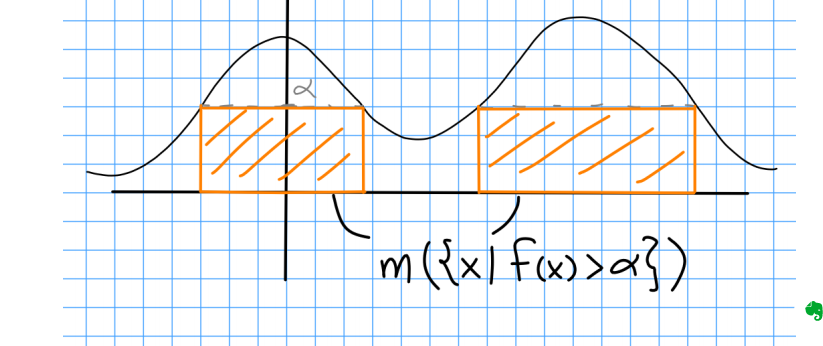
\includegraphics{figures/image_2021-06-02-22-59-46.png}
\caption{image\_2021-06-02-22-59-46}
\end{figure}

The probability interpretation:
\({\mathbb{P}}(X\geq \alpha) \leq {1\over \alpha} {\mathbb{E}}(X)\).

The more general version:
\begin{align*}
\mu \qty{ f^{-1}\qty{(\alpha, \infty)} } \coloneqq\mu\qty{\left\{{ x\in X {~\mathrel{\Big|}~}{\left\lvert {f(x)} \right\rvert} > \alpha }\right\}  } \leq {1\over \alpha^p} {\left\lVert {f} \right\rVert}_p^p \coloneqq{1\over \alpha^p} \int_X {\left\lvert {f} \right\rvert}^p 
.\end{align*}
Proof:
\begin{align*}
{\left\lVert {f} \right\rVert}_p^p = \int {\left\lvert {f} \right\rvert}^p \geq \int_{S_\alpha} {\left\lvert {f} \right\rvert}^p \geq \alpha^p \int_{S_\alpha} 1 = \alpha^p \mu(S_\alpha)
.\end{align*}

\end{proposition}

\begin{proposition}[Minkowski's Inequality]

\begin{align*}  
1\leq p < \infty \implies {\left\lVert {f+g} \right\rVert}_{p} \leq {\left\lVert {f} \right\rVert}_{p}+ {\left\lVert {g} \right\rVert}_{p}
.\end{align*}

\end{proposition}

\begin{remark}

This does not handle \(p=\infty\) case. Use to prove \(L^p\) is a normed
space.

\end{remark}

\begin{proof}[of Minkowski's inequality]

\envlist

\begin{itemize}
\item
  We first note
  \begin{align*}  
  {\left\lvert {f+g} \right\rvert}^p = {\left\lvert {f+g} \right\rvert}{\left\lvert {f+g} \right\rvert}^{p-1} \leq \left( {\left\lvert {f} \right\rvert} + {\left\lvert {g} \right\rvert}\right) {\left\lvert {f+g} \right\rvert}^{p-1}
  .\end{align*}
\item
  Note that if \(p,q\) are conjugate exponents then
  \begin{align*}  
  \frac 1 q &= 1 - \frac 1 p = \frac{p-1} p \\
  q &= \frac p {p-1} 
  .\end{align*}
\item
  Then taking integrals yields
  \begin{align*}  
  {\left\lVert {f+g} \right\rVert}_p^p &=
  \int {\left\lvert {f+g} \right\rvert}^p \\
  &\leq \int \left( {\left\lvert {f} \right\rvert} + {\left\lvert {g} \right\rvert}\right) {\left\lvert {f+g} \right\rvert}^{p-1} \\ 
  &= \int {\left\lvert {f} \right\rvert} {\left\lvert {f+g} \right\rvert}^{p-1} + \int {\left\lvert {g} \right\rvert} {\left\lvert {f+g} \right\rvert}^{p-1} \\
  &= {\left\lVert {f(f+g)^{p-1}} \right\rVert}_1 + {\left\lVert {g(f+g)^{p-1}} \right\rVert}_1 \\
  &\leq {\left\lVert {f} \right\rVert}_p ~{\left\lVert {(f+g)^{p-1})} \right\rVert}_q + {\left\lVert {g} \right\rVert}_p ~{\left\lVert {(f+g)^{p-1})} \right\rVert}_q \\
  &= \left( {\left\lVert {f} \right\rVert}_p + {\left\lVert {g} \right\rVert}_p \right) {\left\lVert { (f+g)^{p-1})} \right\rVert}_q \\
  &= \left( {\left\lVert {f} \right\rVert}_p + {\left\lVert {g} \right\rVert}_p \right) \left( \int {\left\lvert {f+g} \right\rvert}^{(p-1)q} \right)^{\frac 1 q} \\
  &= \left( {\left\lVert {f} \right\rVert}_p + {\left\lVert {g} \right\rVert}_p \right) \left( \int {\left\lvert {f+g} \right\rvert}^{p} \right)^{1 - \frac 1 p} \\
  &= \left( {\left\lVert {f} \right\rVert}_p + {\left\lVert {g} \right\rVert}_p \right) \frac{\int {\left\lvert {f+g} \right\rvert}^{p} }{\left( \int {\left\lvert {f+g} \right\rvert}^{p} \right)^{\frac 1 p}} \\
  &= \left( {\left\lVert {f} \right\rVert}_p + {\left\lVert {g} \right\rVert}_p \right)  \frac{{\left\lVert {f+g} \right\rVert}_p^p}{{\left\lVert {f+g} \right\rVert}_p}
  .\end{align*}
\item
  Cancelling common terms yields
  \begin{align*}  
  1 &\leq \left( {\left\lVert {f} \right\rVert}_p + {\left\lVert {g} \right\rVert}_p \right) \frac{1}{{\left\lVert {f+g} \right\rVert}_p} \\
  &\implies 
  {\left\lVert {f+g} \right\rVert}_p
  \leq {\left\lVert {f} \right\rVert}_p + {\left\lVert {g} \right\rVert}_p 
  .\end{align*}
\end{itemize}

\end{proof}

\begin{proposition}[Young's Inequality]

\begin{align*}
\frac 1 p + \frac 1 q = \frac 1 r + 1 \implies
\|f \ast g\|_{r} \leq\|f\|_{p}\|g\|_{q}
\end{align*}

\end{proposition}

\begin{remark}[some useful special cases]

\begin{align*}  
{\left\lVert {f\ast g} \right\rVert}_1      & \leq {\left\lVert {f} \right\rVert}_1 {\left\lVert {g} \right\rVert}_1 \\
\|f * g\|_{p}         & \leq {\left\lVert {f} \right\rVert}_1 {\left\lVert {g} \right\rVert}p, \\
{\left\lVert {f\ast g} \right\rVert}_\infty & \leq {\left\lVert {f} \right\rVert}_2 {\left\lVert {g} \right\rVert}_2 \\
{\left\lVert {f\ast g} \right\rVert}_\infty & \leq {\left\lVert {f} \right\rVert}_p {\left\lVert {g} \right\rVert}_q
.\end{align*}

\end{remark}

\hypertarget{inequalities-that-appear-in-proofs}{%
\subsection{Inequalities that appear in
proofs}\label{inequalities-that-appear-in-proofs}}

\begin{proposition}[AM-GM Inequality]

\begin{align*}
\sqrt{ab} \leq \frac{a+b}{2}
.\end{align*}

\end{proposition}

\begin{proposition}[Jensen's Inequality]

\begin{align*}
f(tx + (1-t)y) \leq tf(x) + (1-t)f(y)
.\end{align*}

\end{proposition}

\begin{proposition}[Young's Product Inequality]

\begin{align*}
AB \leq {A^p \over p} + {B^q \over q}
.\end{align*}

\end{proposition}

\begin{proposition}[?]

\begin{align*}
(a+b)^p \leq 2^{p-1} (a^p + b^p)
.\end{align*}

\end{proposition}

\begin{proposition}[Bernoulli's Inequality]

\begin{align*}
(1 + x)^n \geq 1 +nx \quad x\geq -1, \text{ or } n\in 2{\mathbb{Z}}\text{ and } \forall x
.\end{align*}

As a consequence,
\begin{align*}
1-x \leq e^{-x}
.\end{align*}

\end{proposition}

\begin{proposition}[Exponential Inequality]

\begin{align*}  
\forall t\in {\mathbb{R}},\quad 1 + t \leq  e^t
.\end{align*}

\end{proposition}

\begin{proof}

\envlist

\begin{itemize}
\tightlist
\item
  It's an equality when \(t=0\).
\item
  \({\frac{\partial }{\partial t}\,} 1+ t < {\frac{\partial t}{\partial e}\,}^t \iff t<0\)
\end{itemize}

\end{proof}

\begin{proposition}[Young's Convolution Inequality]

\begin{align*}
{1\over r} \coloneqq{1\over p} + {1\over q} - 1 \implies {\left\lVert {f \ast g} \right\rVert}_{r} \leq {\left\lVert {f} \right\rVert}_{p} {\left\lVert {g} \right\rVert}{q}
.\end{align*}

\end{proposition}


\printbibliography[title=Bibliography]


\end{document}
